\section{Chapter introduction}

Considering its impacts on the energy budget at the surface, the effects of irrigation follow a marked diurnal cycle, with distinct nighttime and daytime effects and varying amplitude depending on insolation. 
%option:could reuse refs from Intro
Average monthly or seasonal studies (like the work presented in Chapter \ref{chap:monthly}) cannot allow a detailed analysis of these impacts, and simulation outputs at a finer temporal resolution must be used.

Using the same simulation setup as Chapter \ref{chap:monthly}, this chapter focuses on the month on July 2021, and on part of the Ebro Valley. This study area and period were selected to include the measurement sites and special observation period (SOP) of the LIAISE field campaign. This enables direct comparison to local observations of temperature, humidity, wind and turbulent fluxes on irrigated and rainfed sites, at the surface and in the boundary layer. Furthermore, mesoscale modelling experiments were conducted over this area and period, in particular one with the mesoscale Meso-NH model at 2-km resolution that accounts for irrigation \citep{lunel_irrigation_2024}. This simulation served as an intermediate between punctual observations and the regional climate model, bringing new perspective on the following questions:

\begin{itemize}
    \item How does the ICOLMDZOR-LAM perform over the LIAISE study area, relative to observations and mesoscale simulation?
    \item To what extent does simulated irrigation improve the performance of the LAM? What limits its ability to reproduce observations on irrigated and rainfed sites at the diurnal scale?
    \item Are the effects of simulated irrigation limited to surface variables or do they propagate to the vertical structure of the ABL? 
    \item Are the effects of simulated irrigation only visible over the irrigated areas or do they also affect neighbouring rainfed areas?
    \item Over such a heterogeneous terrain, how can representativity of the LAM be defined and to what extent is it achieved?
\end{itemize}

This chapter first presents the LIAISE field campaign with details on the measurements and mesoscale simulation used, and relevant results of this project.
Then, the ICOLMDZOR LAM simulations used for comparison over LIAISE sites are described, before presenting results on land-atmosphere coupling variables and the vertical structure of the atmosphere.
%todo: improve/rephrase after final structure

\clearpage

\section{The LIAISE field campaign}
I would like to start by acknowledging that this description of the Land Surface Interactions with the Atmosphere over the Iberian Semi-Arid Environment (LIAISE) project is largely based on the various articles which presented the campaign : \citet{boone_land_2019,boone_updates_2021,boone_land_2025}, as well as on the dedicated section in Tanguy Lunel's PhD thesis \citep{lunel_interactions_2024}.

%objectives
LIAISE is an international research campaign aimed at improving the understanding of land-atmosphere-hydrology interactions in a semi-arid region characterized by strong surface heterogeneity owing to contrasts between the natural landscape and irrigation-dependent agriculture, and the limitations of models to represent all aspects of the terrestrial water cycle.

\subsection{Study area and meteorological conditions}

%period
Although the campaign included a longer monitoring of surface variables, this work focuses on the special observation period (SOP) which occurred from July  15–29 2021. This SOP has been selected since it is the period where contrasts between irrigated and natural surfaces are generally at or near their maximum. At this time, synoptic scale winds are typically light and from the west, and a  therma low pressure area generally forms over the region with daily maximum temperatures between 30 and 40°C.
Within this SOP, Intensive Observation Periods (IOPs) were selected, aiming for relatively clear days characterized by a well-mixed  atmospheric boundary layer with weak synoptic scale forcing, so that surface-induced local to regional scale circulations were most likely to be present and detectable. 

%area
The study domain for LIAISE is the Segre river basin in northeastern Spain. It is located a sub-basin of the Ebro basin, which is bound to the north by the Pyrenees, to the south by the Iberian System, and to the East by the less elevated Catalan Pre-coastal Range (Fig. \ref{fig:liaise_area_both}a).
It presents a semi-arid hot, dry  Mediterranean climate, with a very sharp delineation between a vast, nearly continuous irrigated region and the generally drier rainfed zone to the east of the study domain. The canal d'Urgell is a major irrigation infrastructure in the Segre basin that enables gravitational flooding of the irrigated area and effectively delineates the irrigated and rainfed zones.
More recently, the Segarra-Garrigues canal was been built to the east of the Urgell canal, with the objective of providing water for irrigation in the eastern part of the Segre sub-basin..

\begin{figure}[hbtp]
    \centering
    \begin{subfigure}{\textwidth}
        \centering
        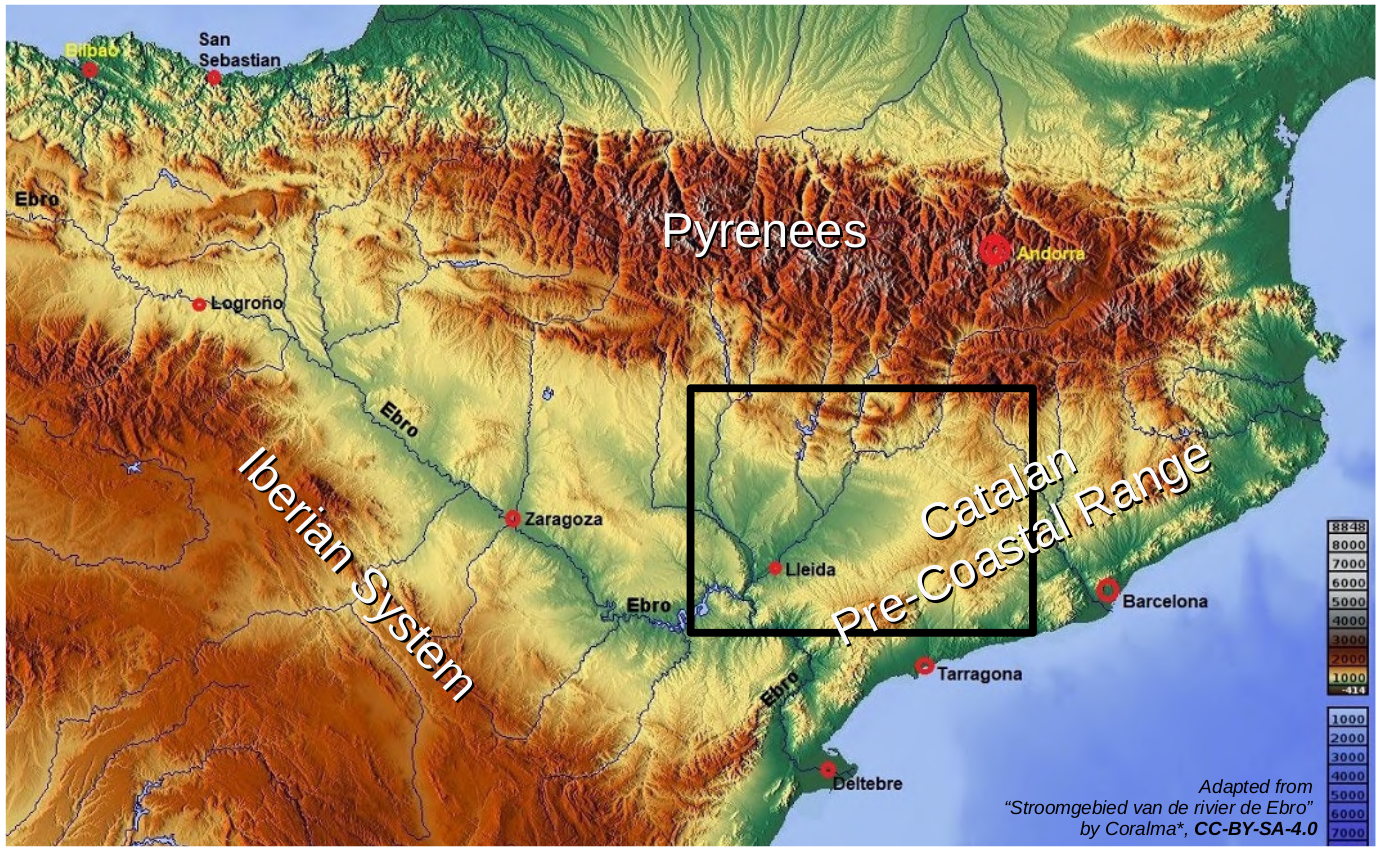
\includegraphics[width=0.8\linewidth]{images/chap5/liaise_area_ebro_lunel.png}
        \caption{Orography of the Ebro basin region. The three mountain ranges are indicated in white, and the black box corresponds to the zoom of (b)}
    \end{subfigure}
    %
    \begin{subfigure}{\textwidth}
        \centering
        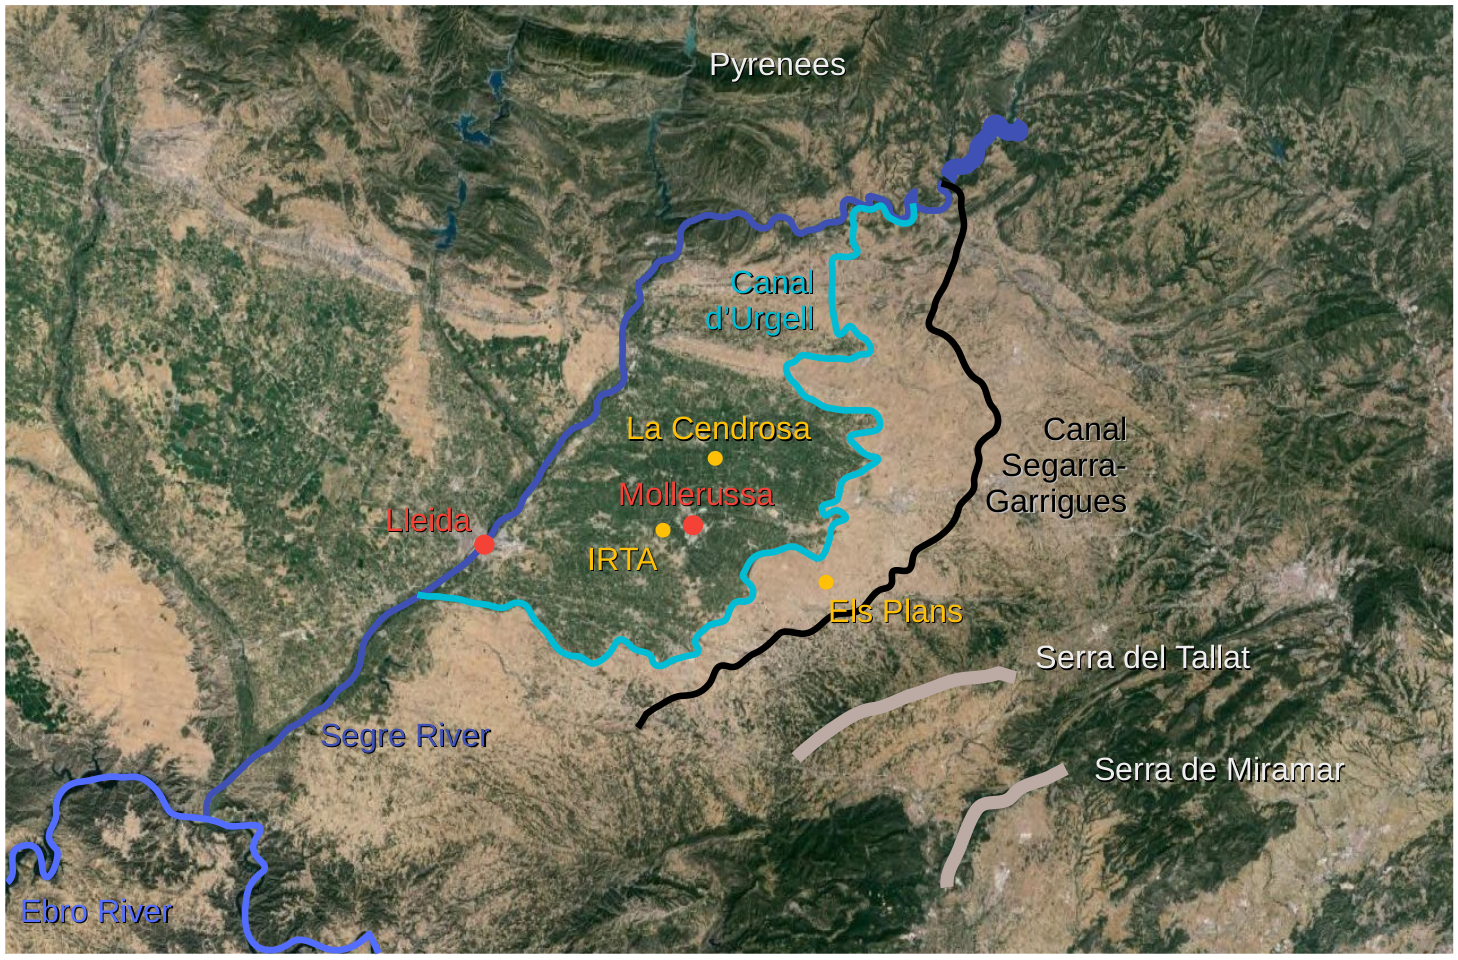
\includegraphics[width=0.7\linewidth]{images/chap5/liaise_area_zoom_lunel.png}
        \caption{Satellite visible image of the Segre river basin and its main topographic features taken by LandSat 7 in July 2021. The Segre and Ebro rivers are shown in dark blue, the Urgell canal in cyan and the recently built Segarra-Garrigues canal in black. The mountain ranges are in light brown. In red are the two main cities of the area and in yellow are the main instrumented sites of the LIAISE campaign.}
    \end{subfigure}
    \caption{Overview of the LIAISE study area. Both figures were taken from\citet{lunel_interactions_2024}.}
    \label{fig:liaise_area_both}
\end{figure}

%sites
Two supersites were defined at La Cendrosa, within the irrigated zone, and Els Plans, within the rainfed zone. Each was equipped with a 50-meter mast to measure temperature, humidity, wind speed and direction, radiative and turbulent fluxes (using eddy-covariance) at various heights.
Here are excerpts from the description of both sites given in \citet{lunel_interactions_2024}:
\begin{quote}
    La Cendrosa is one of the two sites along with Els Plans, which was equipped with numerous instruments to allow an in-depth study of its ecophysiological, soil and meteorological conditions. It is located well inside the heavily irrigated area [...], at an altitude of 240 m a.s.l., and on an almost flat area, with a slope of about 0.5\% towards the west.
    The alfalfa field where the instruments were installed is approximately 300 m x 200 m. Alfalfa is a perennial plant used to feed livestock and can be mown several times (including multiple growth cycles in a single summer). The alfalfa in the field was mown on 5 July 2021 and it regrew progressively over the rest of the month. [...] At the beginning of the two week period, the low LAI of the field affected the Bowen ratio measured above the field. It was observed that the Bowen ratio gradually decreased until it became constant around 21 July (not shown). La Cendrosa was flood irrigated twice in July, on the nights between 10 and 11 and between 23 and 24.
\end{quote}
\begin{quote}
    The site of Els Plans is a rainfed fallow land. It contains very little vegetation, and this vegetation was mainly dry during the SOP. It is located at the foothills of the [Catalonian Pre-coastal Range], on a very gentle slope of about 1\% facing north-northwest, at an altitude of 334 m a.s.l. Els Plans is located about 3 km southeast of the irrigated-dry boundary.
\end{quote}

This work used 2-meter measurements of land-atmosphere coupling variables and 10-m wind (Section \ref{sec:sop}).
On IOP days, hourly radiosondes were launched, roughly from  sunrise through early evening, probing the ABL up to about 3 km. These measurements are used in Section \ref{sec:iop} to analyse the vertical structure of the atmosphere on 15 July and 20th.

Over the SOP, meteorological conditions were described as dry and hot, and only one precipitation event occurred, on 26 July. It was due to a thunderstorm which brought more than 25 mm to La Cendrosa but then propagated northeast and didn't affect the Els Plans site.
%option: wind regimes ? dominant, details on sea breeze...

\begin{figure}[hbtp]
    \centering
    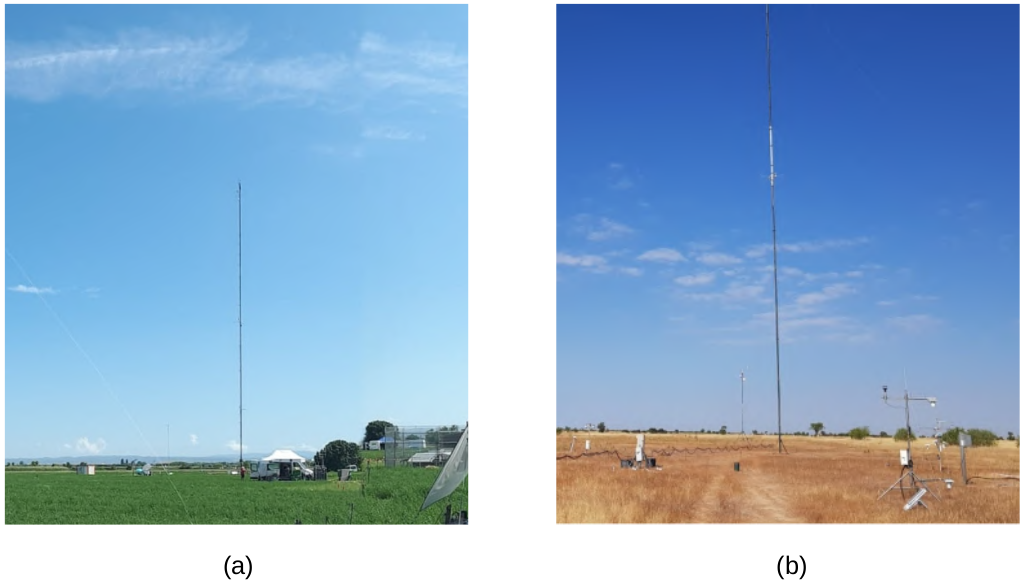
\includegraphics[width=\textwidth]{images/chap5/liaise_sites_picture.png}
    \caption{Instrumented sites of La Cendrosa (a) and Els Plans (b) in July 2021 \citep[taken from ][]{lunel_interactions_2024}.}
    \label{fig:liaise_sites_photos}
\end{figure}

%option: more details on choice of IOP days, synoptic conditions
%  This thermal situation has  a strong impact on surface winds. Formation of some shallow cumulus is possible, but moist convection, if present, is  generally confined to the surrounding mountain ranges. Owing to the proximity to the Mediterranean Sea to the east, sea  breeze (SB) formation is quite frequent, but its inland progression is slowed by the presence of the Catalan pre-coastal and  coastal ranges that separate the Ebro basin from the sea. The  intensity of the westerlies and strength of the heat low are also  contributing factors to the SB front propagation and intensity. Generally speaking, the SB front usually arrived sometime  between 16:00 and 19:00 local time over the study zone with  the dry zone sites impacted earliest. The SB passage was seen  in the observations as a low level wind shift (to winds with a  significant easterly component) over the entire region, while in  the east, horizontally-scanning lidar observations also revealed  a significant increase in low-level moisture with its arrival. The  sea breeze generally coincided with a collapsing ABL in the late  afternoon. Days with a predicted early arrival of the SB were  not designated as IOPs during the daily briefings. Finally, one  rain event did occur on July 26, which was associated with the  passage of a synoptic scale trough: local precipitation totals of  around 30 mm were recorded over the irrigated zone; however,  the convective cells propagated to the northeast and the dry zone received relatively little rainfall, thereby reinforcing the  wet-dry zone contrast during the subsequent days of the SOP.

\subsection{First results from observations and modelling}

The observations data from the LIAISE project has already been used in comparisons to mesoscale models to assess the relevance of simulating irrigation. 

The multi-model comparison presented in \citet{jimenez_land-surface_2025}, analysed simulations with Meso-NH  \citep{lac_overview_2018}, the Unified Model \citep{bush_second_2023,walters_met_2017} and WRF \citep{skamarock2021description} over the region. This study was initiated before the campaign took place and simulations were conducted without irrigation. It identified limitations of all models over the irrigated portions of the study area and concluded "that it is important to take this process into account in order to capture land-atmosphere interactions properly".

Later, \citet{lunel_irrigation_2024} conducted simulations with and without irrigation, with the Meso-NH modelat 400-meter, nested into a larger Meso-NH simulation at 2-kilometer resolution. 
In these simulations, irrigation is represented in the SURFEX LSM \citep[Surface Externalisée][]{masson_surfexv72_2013} by identifying irrigated areas in the land cover input map to associate them to a higher LAI, and by maintaining soil moisture at field capacity on those areas throughout the simulation.
On 20 and 22 July, it showed very significant improvement of simulated near-surface conditions at La Cendrosa when using irrigation, with a 4.7°C decrease in 2-meter temperature and a 50\% increase in 2-meter specific humidity during the day. The impacts of irrigation were not confined to surface variables but also influenced the structure of the ABL, achieving more stable profiles over La Cendrosa which matched the radiosoundings at 12UTC on both days. 
Tanguy Lunel kindly provided the outputs from the 2-kilometer simulation with irrigation, which were used as a gridded reference in complement to the punctual observations of the campaign and allowed for the exploration of sub-grid heterogeneities in ICOLMDZOR, as presented in the following sections.

In a similar setup with the WRF model, \citet{udina_irrigation_2024} also found better model performance for near-surface air temperature, humidity, and wind speed and direction when the model included the irrigation parametrization. They noted lowering of the ABL around irrigated areas and a weakening of the sea breeze circulation, which is also described in \citet{lunel_marinada_2024}.
However, irrigation was not associated with a better representation of precipitation over the SOP (mainly the thunderstorm on 26 July) which was mostly driven by large-scale processes.

LIAISE data was also used to study the evolution of the ABL, with \citet{brooke_irrigation_2023} highlighting the high impact of the contrasts induced by irrigation through the morning transition. 
\citet{mangan_evapotranspiration_2023} studied three scales of heterogeneity (10 km, 1 km, 100 m), to characterize their impact on surface energy partitioning and evapotranspiration, using the atmospheric mixed layer, slab model Chemistry Land-surface Atmosphere Soil Slab model \citep[CLASS, \url{https://classmodel.github.io/}][]{arellano_atmospheric_2015}. They found surface-driven processes (radiation, surface layer) to be more important drivers of ET at the local scale that at the regional one, compared to boundary layer feedbacks. 
Combining this conceptual framework with additional LIAISE observation data, \citet{mangan_surface-boundary_2023} concluded that the observed ABL height was mostly determined by surface fluxes at the regional scale (~10km) rather than local one (~100m), and that non-local boundary layer feedbacks also impacted local surface fluxes.

\hfill

All these results raised interest and questions on the ability of a regional climate model such as the ICODLMZOR LAM to capture the impacts of irrigation on land-atmopshere coupling processes over the LIAISE study area, particularly considering the very limited representation of sub-grid heterogeneity in LMDZ and ORCHIDEE.

\clearpage

\section{Simulation experiments with ICOLMDZOR}

Several simulations are compared to analyse the diurnal cycle of land-atmosphere coupling variables in the Ebro Valley.
First, the two simulations studied in Section \ref{sec:article1} (\noirr and \irr) were analysed and compared to LIAISE observations using hourly outputs over the month of July 2021.

Then, sensitivity experiments were conducted to increase irrigation over grid cell corresponding to the irrigated site of La Cendrosa, leading to the simulation henceforth referred to as \irrboost. This simulation was only run over the month of July, starting from the same state as \noirr and \irr on July 1st 2021, and involved significant changes in both on the computation of irrigation demand, and on the water availability. 
Regarding demand, the irrigated fraction was slightly increased to make sure that all of the soiltile dedicated to low vegetation and crops was considered as irrigated land. This soiltile represents 83.5\% of the grid cell, the rest being occupied by trees (12.4\%) and bare soil (4.1\%). This fraction was also reduced to 0\% on the Els Plans site to make sure there would be no irrigation demand computed in this grid cell.
More importantly, the \betairrig parameter, which had been set to 0.6 after the offline calibration in Chapter \ref{chap:routing} to avoid excessive depletion of the groundwater and river reservoirs, was increased to 1. This means that the irrigation scheme is aiming to maintain soil moisture in the root zone (first 64cm of soil) to field capacity, making sure that plants would not be limited in their growth by available soil moisture. 
Regarding available water, since this was a short simulation run (one month), very large amounts of water were added in the three routing reservoirs at the initial state of the simulation, making virtually inifinite amounts of water available for irrigation in the LIAISE region. Obviously, this method is not realistic, nor applicable to longer climate runs, and was only used to test the limits of the irrigation scheme and explore the sensitivities of land-atmosphere interactions in a context where irrigation would be driven by the water demand rather than the supply. 
When comparing to reality, this can also be seen as a way to compensate for the absence of water adduction in the ICOLMDZOR LAM simulations, a practice that is determinant in the actual supply of irrigated water in the area. 
%todo:see if this explained in previous sec, refer to it
%todo:see also if irrigation simulation method used by tanguy has been detailed (because that's what it does too)
The differences in simulated irrigation between \irr and \noirr are shown on Fig. \ref{fig:sop_irrigation_orchidee} and will later be discussed in Section \ref{sec:sop}.

%fig:irrigation in irr and irr_boost
\begin{figure}[hbtp]
    \centering
    \begin{tabular}{cc}
        \begin{subfigure}[t]{0.5\textwidth}
            \caption{}
            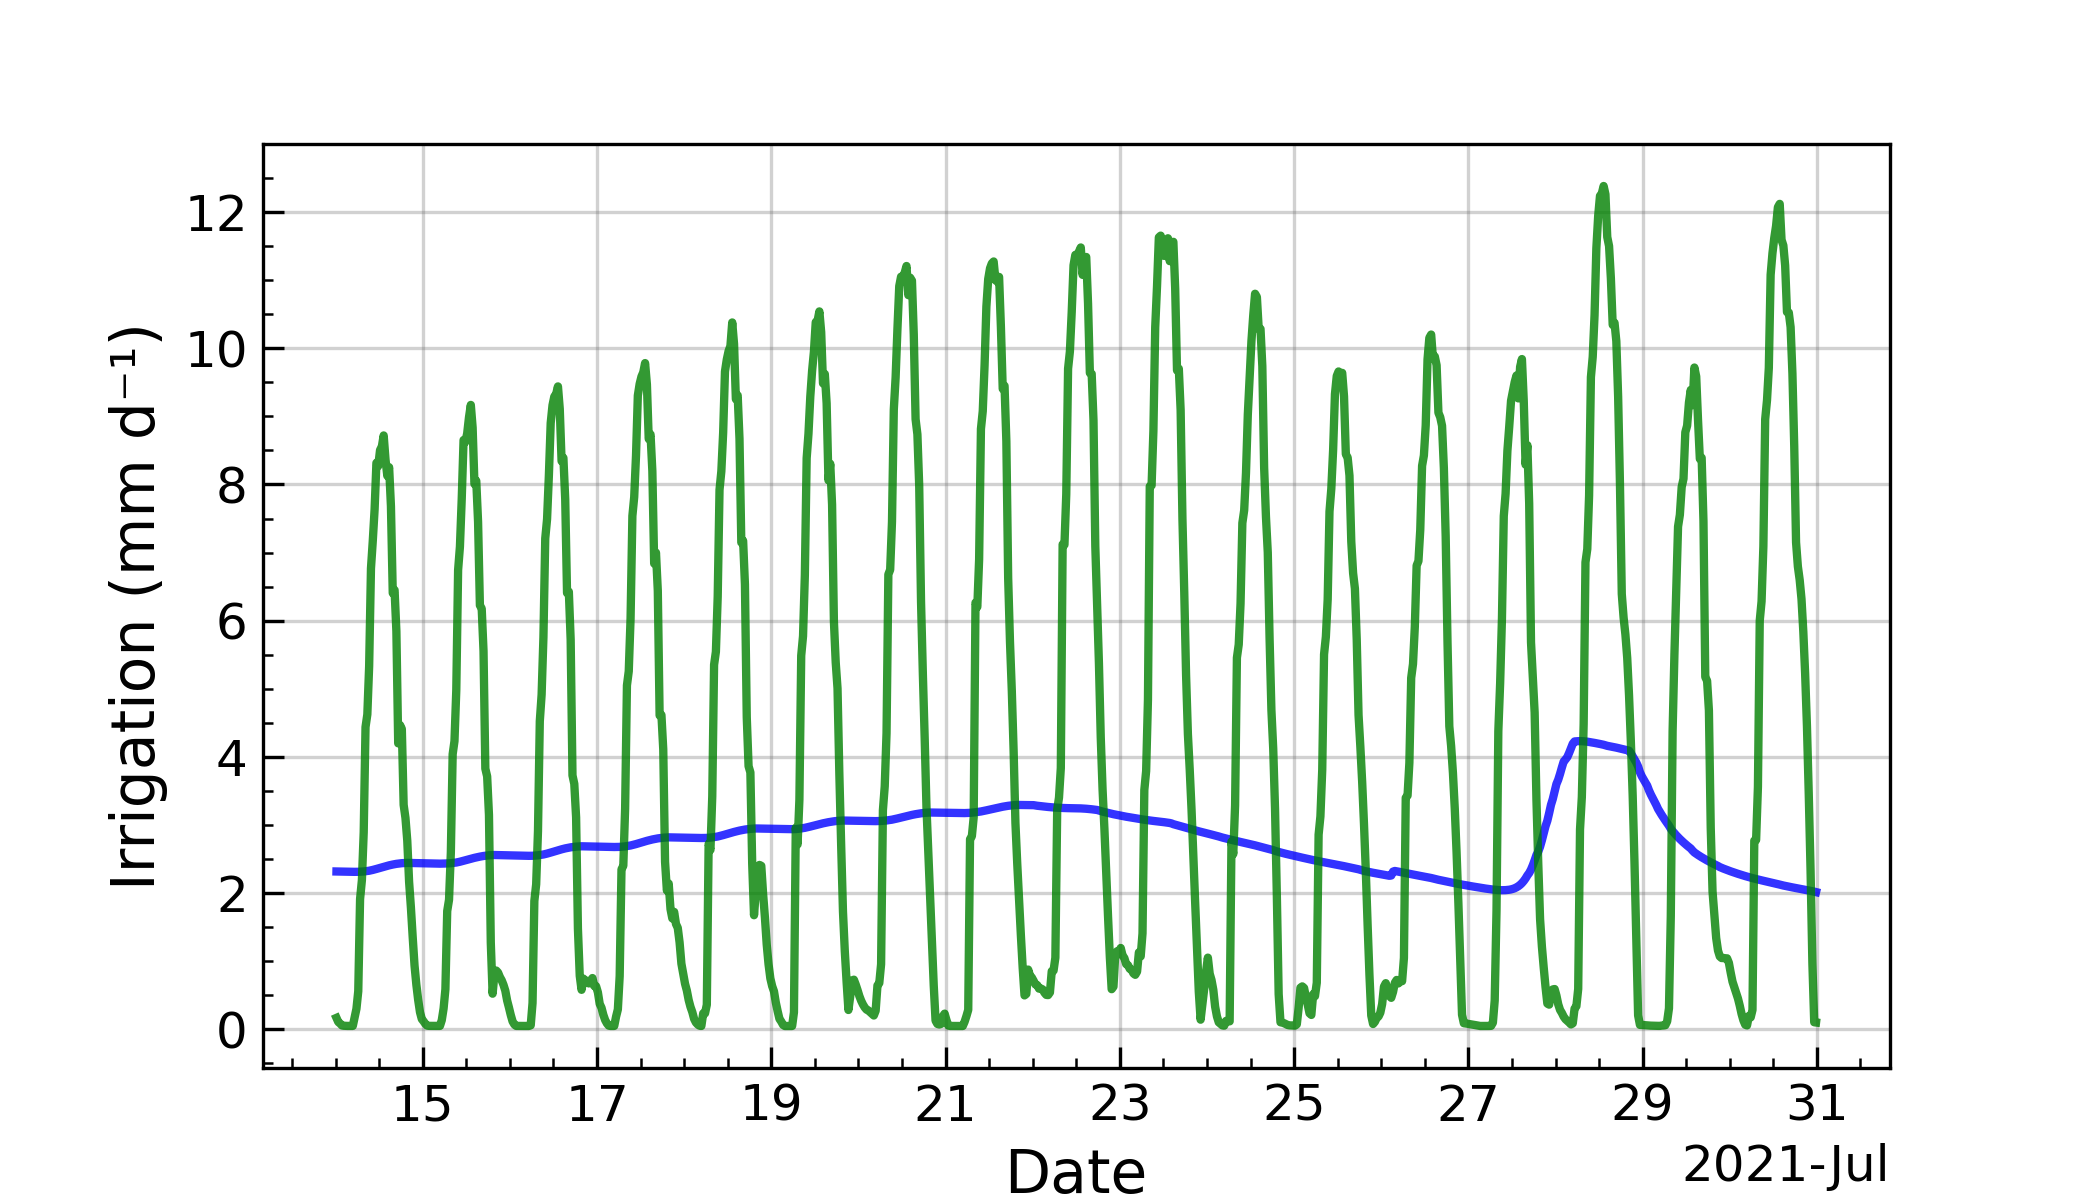
\includegraphics[width=\textwidth]{images/chap5/SOP_TS_DC/time_series_cendrosa_irrigation.png}
        \end{subfigure} &
        \begin{subfigure}[t]{0.5\textwidth}
            \caption{}
            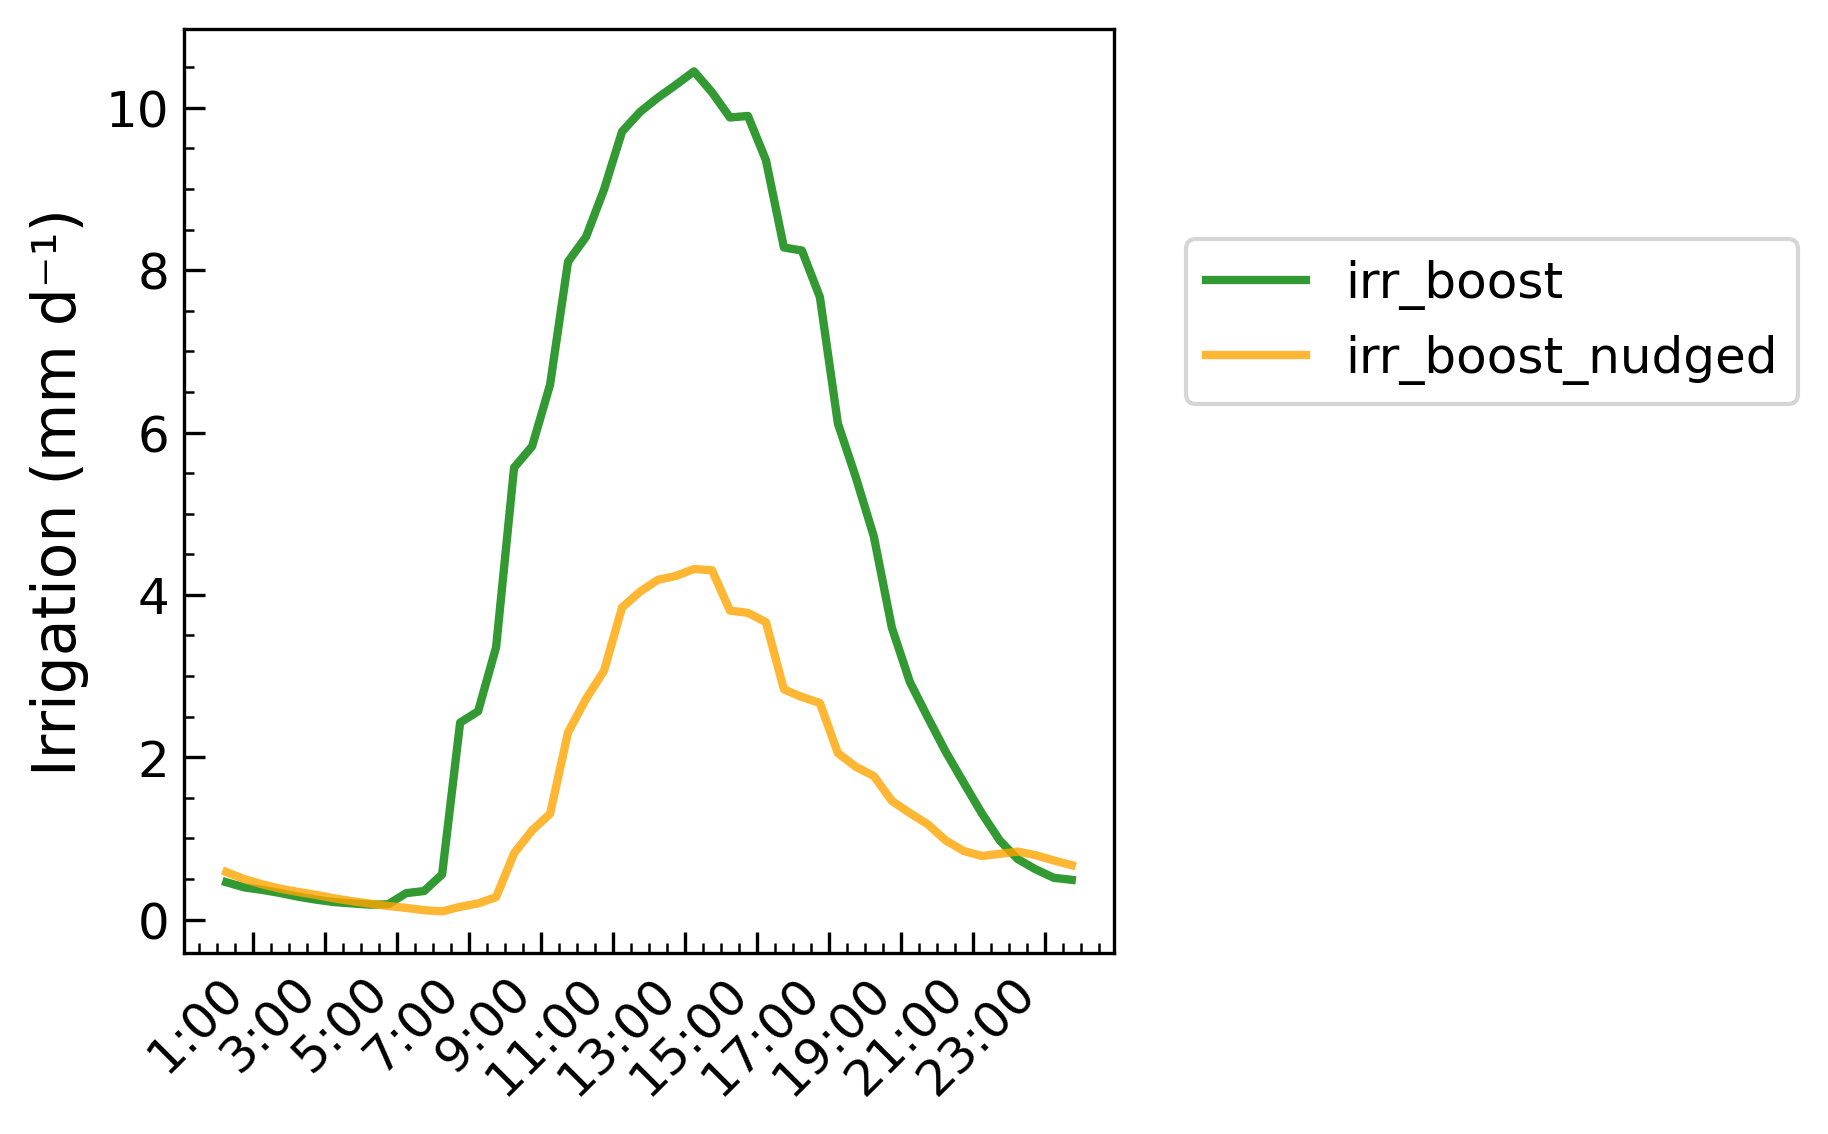
\includegraphics[width=\textwidth]{images/chap5/SOP_TS_DC/diurnal_cycle_cendrosa_irrigation.png}
        \end{subfigure}
    \end{tabular} 
    \caption{Time series and mean diurnal cycle  of simulated irrigation at La Cendrosa in \irr and \irrboost simulations, 14-30 July.}
    \label{fig:sop_irrigation_orchidee}
\end{figure}

\hfill

The three ICOLMDZOR LAM simulations (\noirr, \irr, \irrboost) are compared to observations and to the Meso-NH simulation from 14 to 30 July. This covers all the LIAISE SOP and allows for the stabilization of irrigation volumes in the \irrboost simulation, since no long-term spinup was conducted with this setup.
For each site, an ICOLMDZOR grid cell was selected for the comparison to observations. At Els Plans, the grid cell containing the exact site location seemd appropriate since it was a very lightly irrigated cell. however, the exact position of the La Cendrosa site was not in an intensely irrigated cell, which is why the neighbouring grid cell was selected.

%fig:sites and corresponding grid cells
\begin{figure}[hbtp]
    \centering
    \begin{tabular}{cc}
        \begin{subfigure}[t]{0.44\textwidth}
            \caption{Visible image of the LIAISE study area as seen by \textit{Sentinel-2} on 22 July 2021.}
            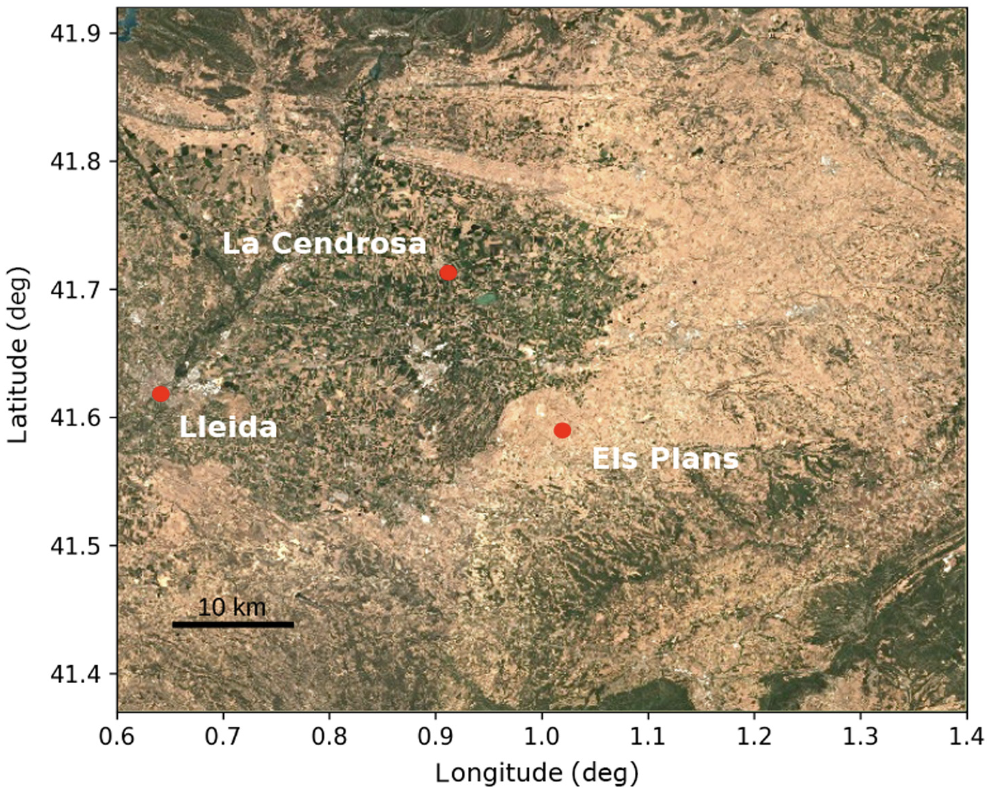
\includegraphics[width=\textwidth]{images/chap5/liaise_overview_lunel.png}
        \end{subfigure} &

        \begin{subfigure}[t]{0.5\textwidth}
            \caption{Monthly average irrigation simulated by ORCHIDEE (July 2021, \irr simulation).}
            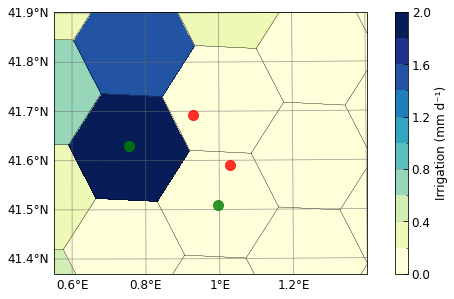
\includegraphics[width=\textwidth]{images/chap5/liaise_sites_irrig_ORC.png}
        \end{subfigure} 
    \end{tabular} 

    \begin{subfigure}[t]{0.75\textwidth}
            \caption{Average latent heat flux simulated by Meso-NH (14-30 July 2021, with irrigation). Red hexagons show the ICOLMDZOR grid cells for each site.}
            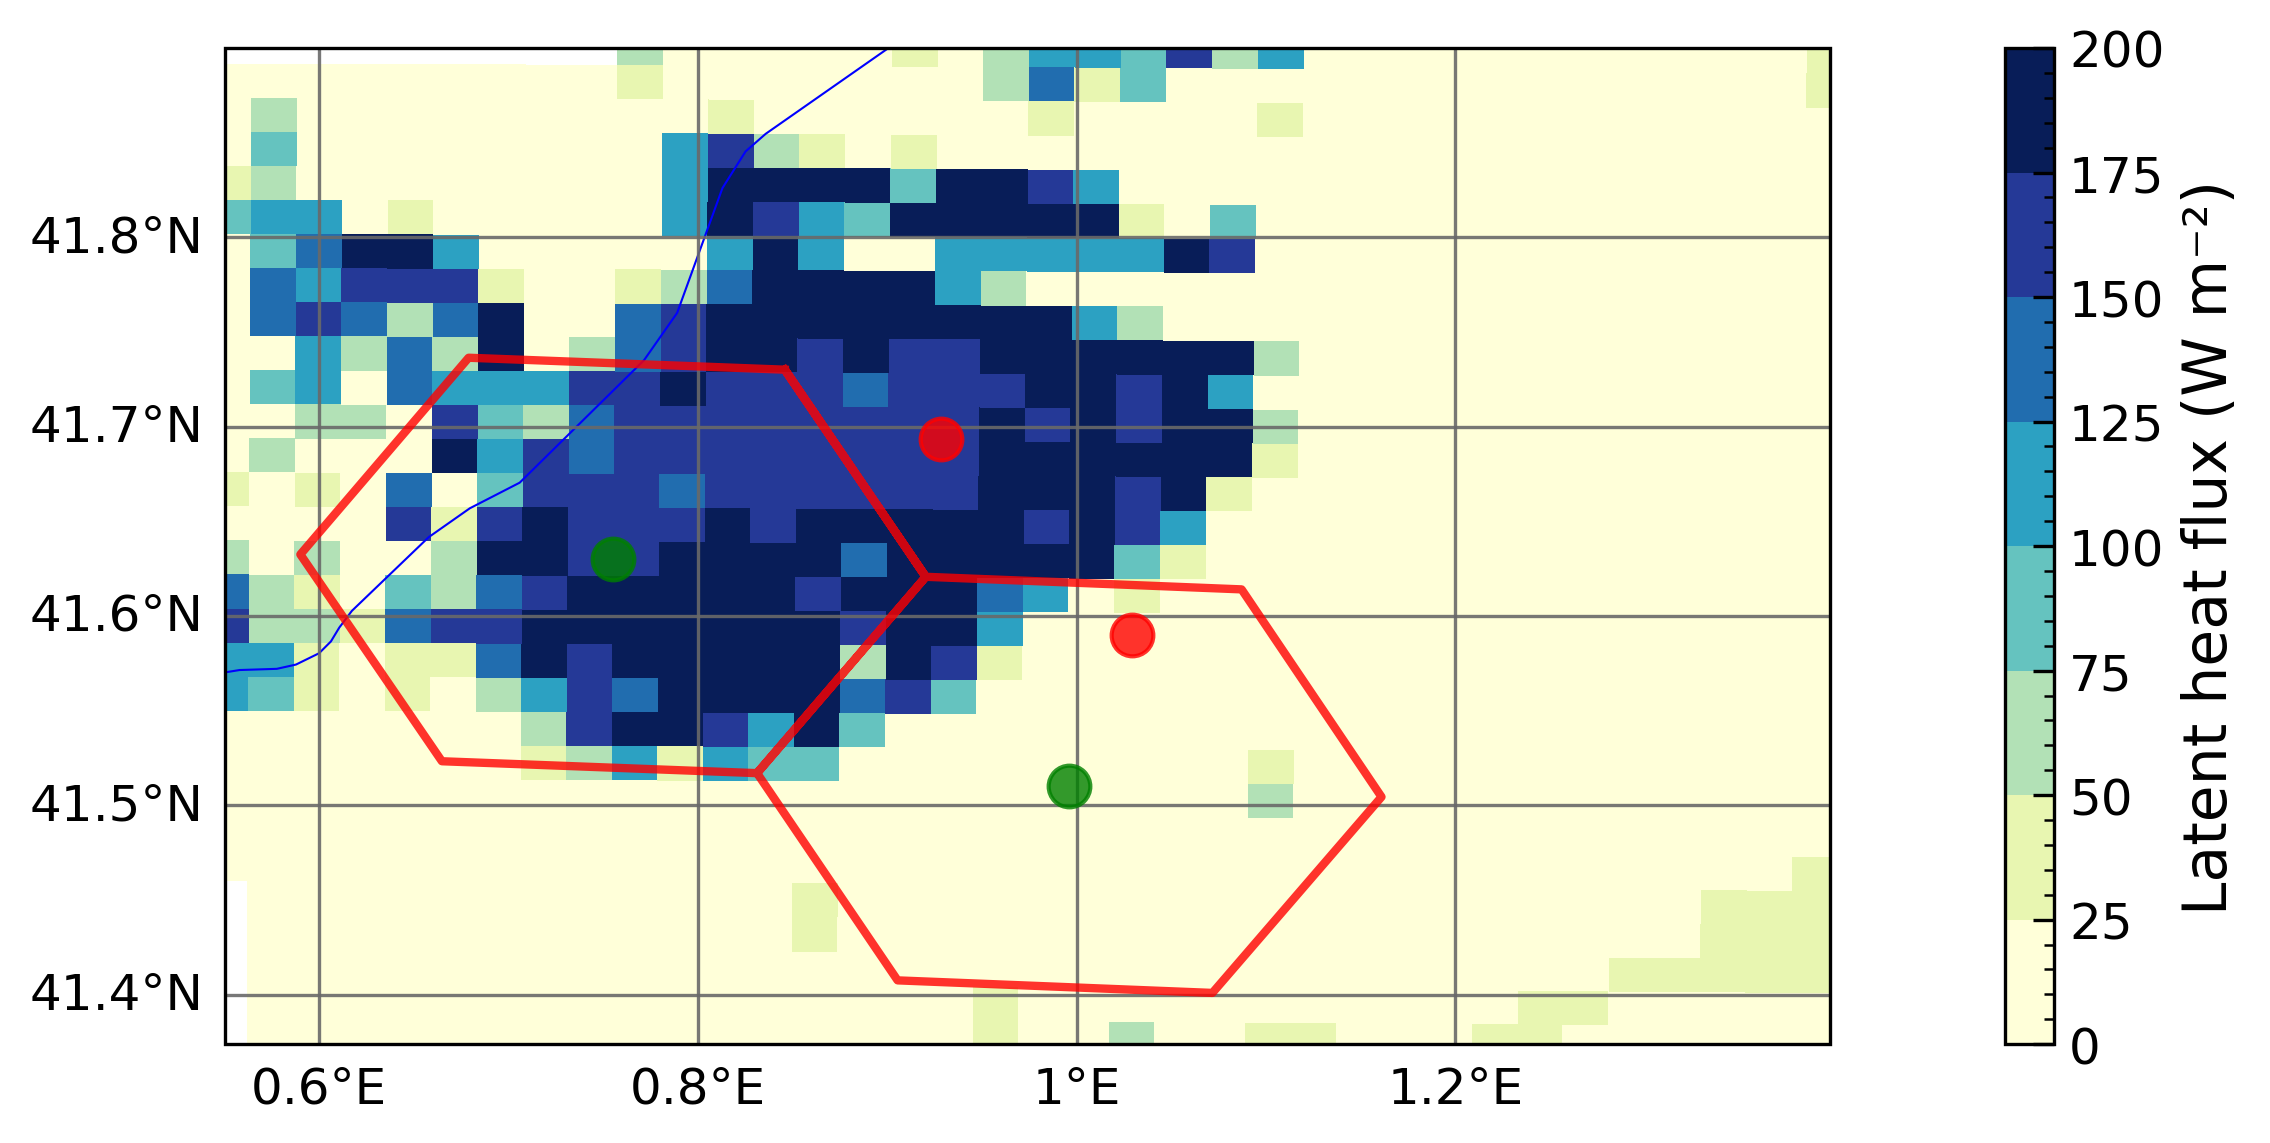
\includegraphics[width=\textwidth]{images/chap5/liaise_sites_mean_mesoNH.png}
        \end{subfigure} 
    
    \caption{Correspondance between actual location of La Cendrosa and Els Plans sites (red dots), selected ICOLMDZOR grid cells (centered on green dots), and Meso-NH grid. (a) was taken from \citet{lunel_irrigation_2024}.}
    \label{fig:liaise_sites_grid_cells}
\end{figure}

%todo:mesoNH (if not presented in previous section ?)
Comparison to the Meso-NH simulations was performed using two values for each site. 
The first one, referred to as \mesoexact, takes the variables from the exact grid cell corresponding to the site location based on the GPS coordinates of the site, as done in \citet{lunel_irrigation_2024}. 
The second, referred to as \mesomean, is an aggregation of all the Meso-NH grid cells contained into the selected ICOLMDZOR grid cell for each site. The mean value is shown, as well as an envelope encompassing the 25th and 75th percentiles, when it is appropriate.
On Fig. \ref{fig:liaise_sites_grid_cells}c, the two hexagonal ICOLMDZOR grid cells are drawn upon the average latent heat flux simulated by Meso-NH. It can already be noticed that within the grid cell for La Cendrosa, there are some Meso-NH grid cells with very low values of ET, and that in the grid cell for Els Plans, there are some Meso-NH grid cells which fall into the irrigated zone and exhibit high ET. This will have an influence on the \mesomean values and on the spread of Meso-NH surface variables within one ICOLMDZOR grid cell. 
%option:mesoMean is not meant to be more representative of the obs than mesoExact, but to bring information on heterogeneity within one ICOLMDZOR grid cell

\section{Near-surface variables over the SOP}
\label{sec:sop}

Here, surface variables simulated by ICOLMDZOR and Meso-NH are compared to the observations on both sites from 14 to 30 July, the span of the Meso-NH simulation, which corresponds to the LIAISE SOP.

\hfill
%%LA CENDROSA%%

At La Cendrosa (Fig. \ref{fig:cendrosa_surfacevars}), observed turbulent fluxes(in black) exhibit a clear diurnal cycle driven by solar irradiation, with a maximum value between 12 and 13UTC.
In the \noirr simulation (in red), ICOLMDZOR simulates a negligible latent heat flux (Fig. \ref{fig:cendrosa_surfacevars}b) and largely overestimates the sensible heat flux (+300\% at 12UTC on Fig. \ref{fig:cendrosa_surfacevars}d). 
These major biases are partly improved in the \irr simulation (in blue), showing that additional soil moisture brought by irrigation can really improve turbulent fluxes. However, latent heat flux simulated in \irr follows a good trajectory from 5UTC to 9UTC but then drops and remains largely underestimated until the evening. This is due to a failure of the irrigation parametrization which cannot sustain the irrigation demand throughout the day since the routing reservoirs (particularly the river reservoirs) cannot provide sufficient irrigation withdrawals. In \irr, the irrigation volume is nearly constant throughout the day (Fig. \ref{fig:sop_irrigation_orchidee}) because the soil moisture deficit is always large but the water withdrawals are capped by available water.
In the \irrboost sensitivity experiment (in green), there is an effectively infinite supply of water in the reservoirs, which allows irrigation to follow a structured diurnal cycle (Fig. \ref{fig:sop_irrigation_orchidee}) and removes the constraint of soil moisture on ET. Both turbulent fluxes follow a diurnal cycle that is consistent with observations, although a small underestimation of latent heat flux and an overestimation of sensible heat flux remain compared to the observations. 
However, the turbulent fluxes in \irrboost are very close to those of \mesomean (in yellow, with the envelope representing the 25th and 75th percentiles of the distribution), suggesting that ICOLMDZOR correctly represents the average fluxes over the grid cell, which does not only include intensely irrigated areas.
It can be noted here that \mesoexact (in purple), corresponding to the exact Meso-NH grid cell of the observation site, overestimates latent heat flux on average over the period. This is mostly due to the beginning of the SOP, where the alfalfa crops at La Cendrosa were still freshly cut and had not recovered their original size, LAI and transpiration levels.

The diurnal cycle of 2-meter temperature is also driven by solar irradiation but its shape is slightly shifted with a peak in the afternoon around 4UTC (Fig. \ref{fig:cendrosa_surfacevars}f). Figure \ref{fig:cendrosa_surfacevars}e shows that temperatures were consistently rising throughout the SOP, from 15 July to 22nd, and that this evolution is well captured by ICOLMDZOR and Meso-NH.
On average over the SOP, all simulations exhibit a warm bias, of at least 1.5° at night, where \mesoexact is closer to ICOLMDZOR than to observations, and of varying amplitude during the day. The \irr simulation has the strongest warm bias, which is consistent with the simulated turbulent fluxes, and this bias is slightly reduced in \irr. In \irrboost, it is largely improved, with a peak temperature 2°C lower than \irr, and simulated values that follow \mesomean throughout most of the day. In the evening, \irrboost even falls closer to observed values than to \mesomean, which suggests that if turbulent fluxes are correctly simulated, the structural nighttime warm bias is smaller in ICOLMDZOR than in Meso-NH.
The diurnal cycle for 2-meter specific humidity is less structured than turbulent fluxes or temperatures.
On Fig. \ref{fig:cendrosa_surfacevars}h, Meso-NH appears to present a dry bias a night, with an underestimation of specific humidity in \mesoexact as strong as in \mesomean. With ICOLMDZOR, a similar bias is present in \noirr, but it is absent in \irr and \irrboost, likely thanks to local ET enabled by irrigation.
In daytime, \mesoexact matches observed values from 8UTC to 18UTC, and \mesomean follows a similar structure through the diurnal cycle. 
ICOLMDZOR, on the contrary, presents an incorrect diurnal cycle of specific humidity, with an extensive drying in daytime. The strength of this drying is largest in \noirr but \irrboost still falls below the values of \mesomean, at the limit of the 25th percentile. 
The differences between ICOLMDZOR and observed values increase largely from 20 July, where humidity drops in the simulations but not in reality or in Meso-NH simulation (Fig. \ref{fig:cendrosa_surfacevars}g).
This shows that in certain daytime conditions, increasing ET by accounting for irrigation is not sufficient to simulate a realistic 2-meter specific humidity. In particular, incorrect advection terms and surface wind can neutralise the effect of this local improvement of land-atmosphere interactions.

This hypothesis is corroborated by the 10-meter wind regime at La Cendrosa (Fig. \ref{fig:bothsites_wind}a-d), which is quite well structured in the beginning of the SOP with low wind speeds, but shows important variations in direction and an increased wind speed from 20 July. ICOLMDZOR seems to be capturing the variations quite well until 19 July but clearly misses part of the regime changes afterwards. 
On average over the SOP, \mesoexact follows observations closely, and the diurnal cycle simulated by ICOLMDZOR has the same structure as \mesomean, particularly for wind direction.
Irrigation only has an impact on the 10-meter wind speed: in \noirr it is overestimated, and that bias is partly reduced in \irr and \irrboost. This was expected since in the presence of irrigation, the vegetation is more developed and LAI is larger, leading to a larger surface drag and therefore lower surface wind speed. 
Wind direction is not impacted by irrigation (red, blue and green lines overlap in Fig. \ref{fig:bothsites_wind}d), which was also expected since only a few grid cells are intensely irrigated in the region, which limits the possibilities of influencing the dynamics of the LAM.

%fig : Cendrosa turbulent fluxes + t2m, q2m
\begin{figure}[hbtp]
    \centering
    \begin{tabular}{cc}
        \begin{subfigure}[t]{0.5\textwidth}
            \caption{}
            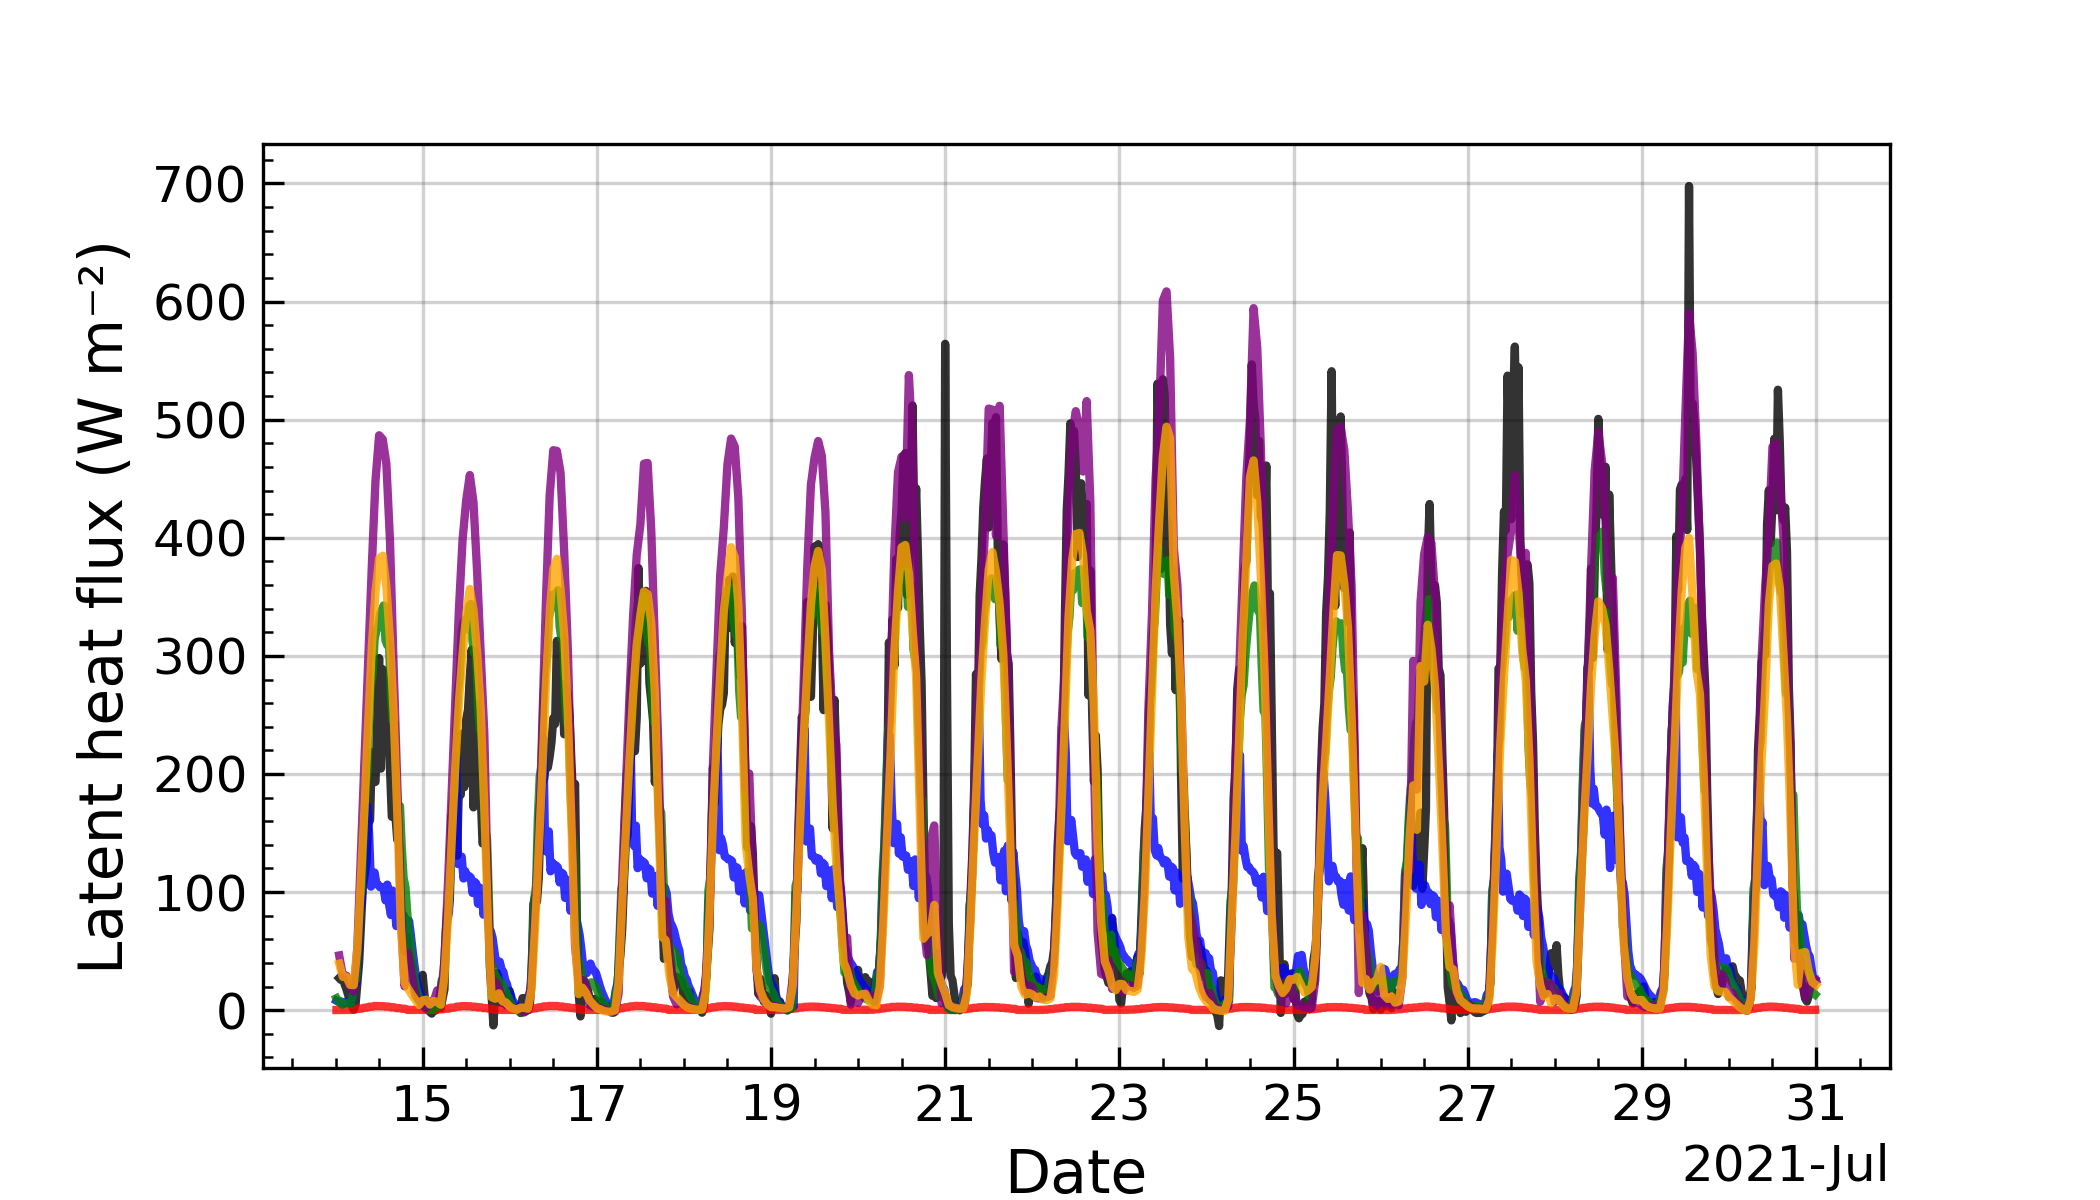
\includegraphics[width=\textwidth]{images/chap5/SOP_TS_DC/time_series_cendrosa_flat.png}
        \end{subfigure} &
        \begin{subfigure}[t]{0.5\textwidth}
            \caption{}
            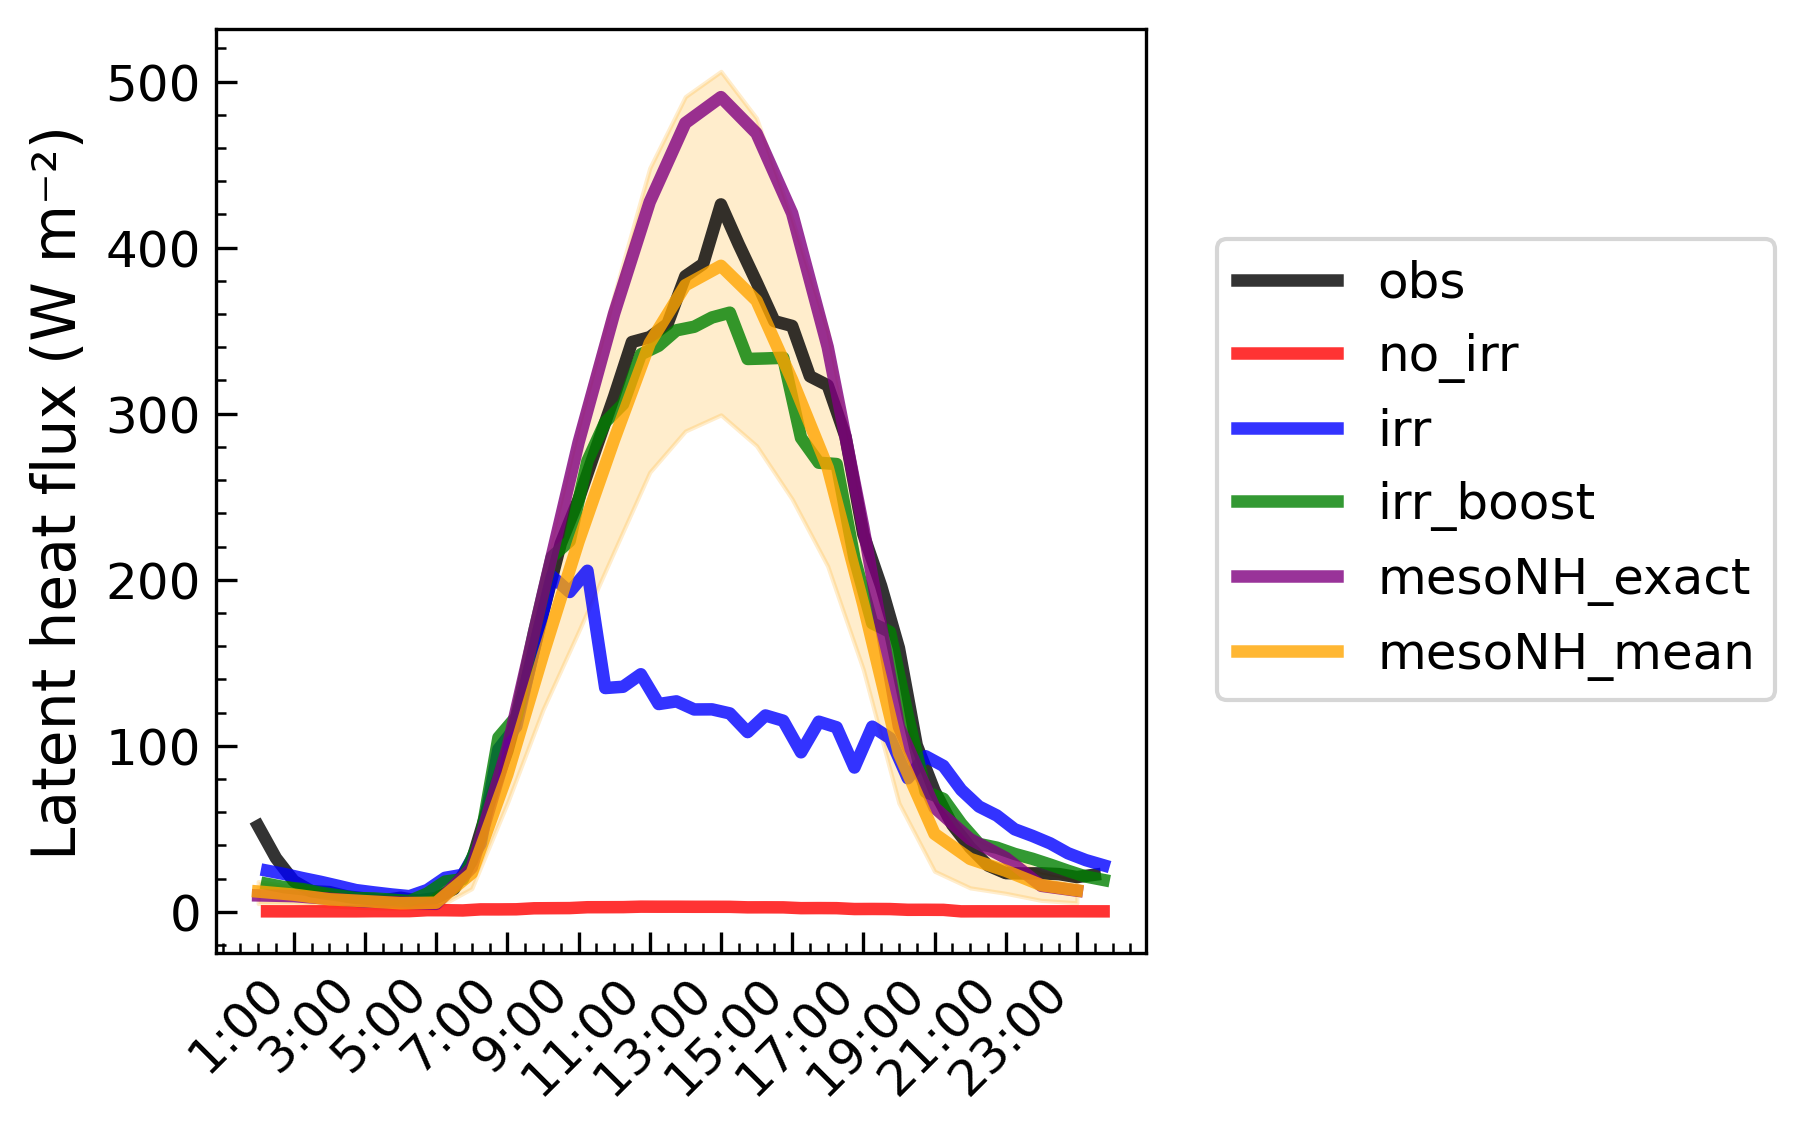
\includegraphics[width=\textwidth]{images/chap5/SOP_TS_DC/diurnal_cycle_cendrosa_flat.png}
        \end{subfigure} \\
        \begin{subfigure}[t]{0.5\textwidth}
            \caption{}
            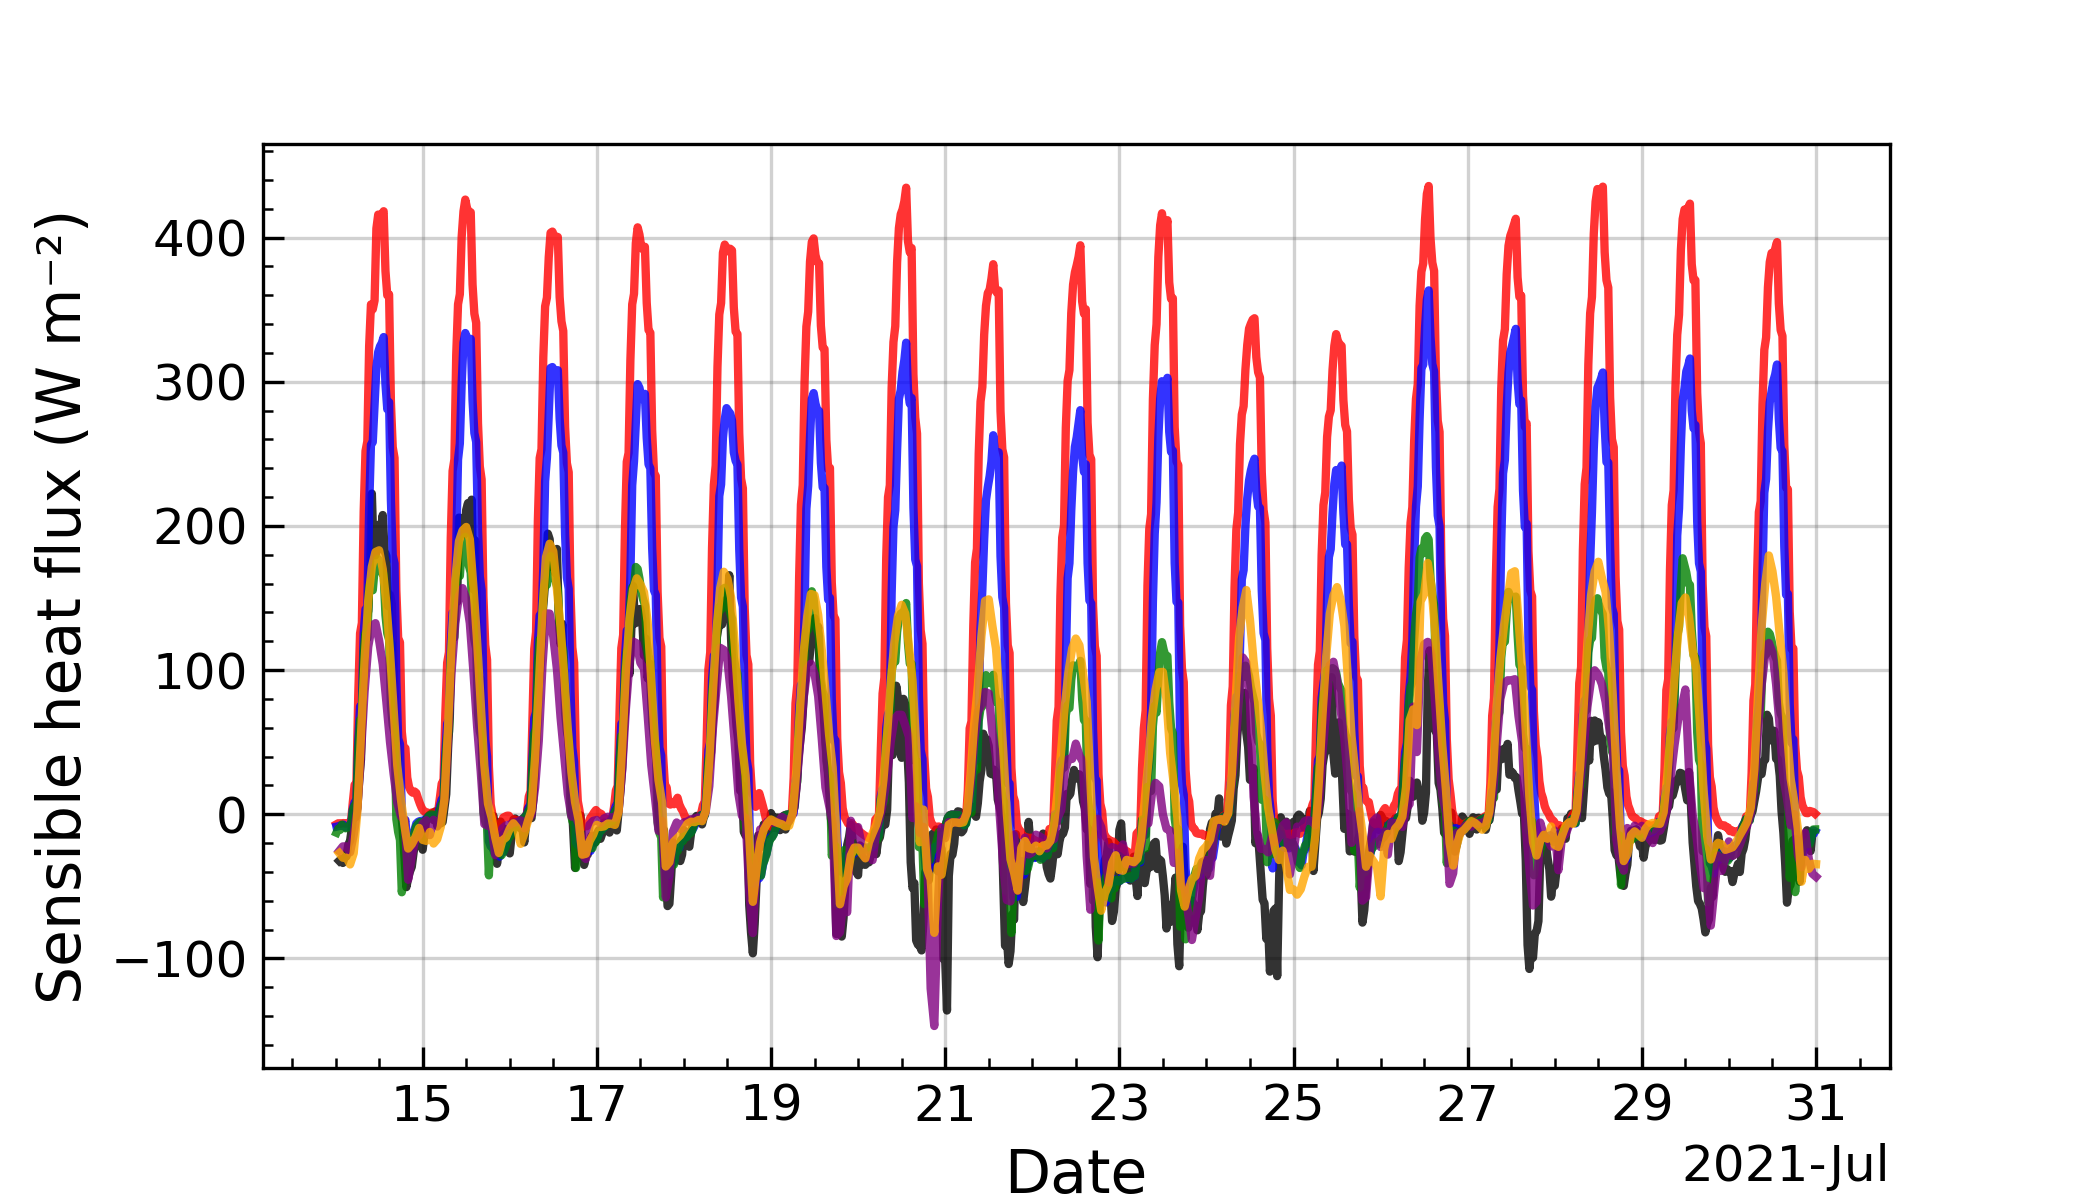
\includegraphics[width=\textwidth]{images/chap5/SOP_TS_DC/time_series_cendrosa_sens.png}
        \end{subfigure} &
        \begin{subfigure}[t]{0.5\textwidth}
            \caption{}
            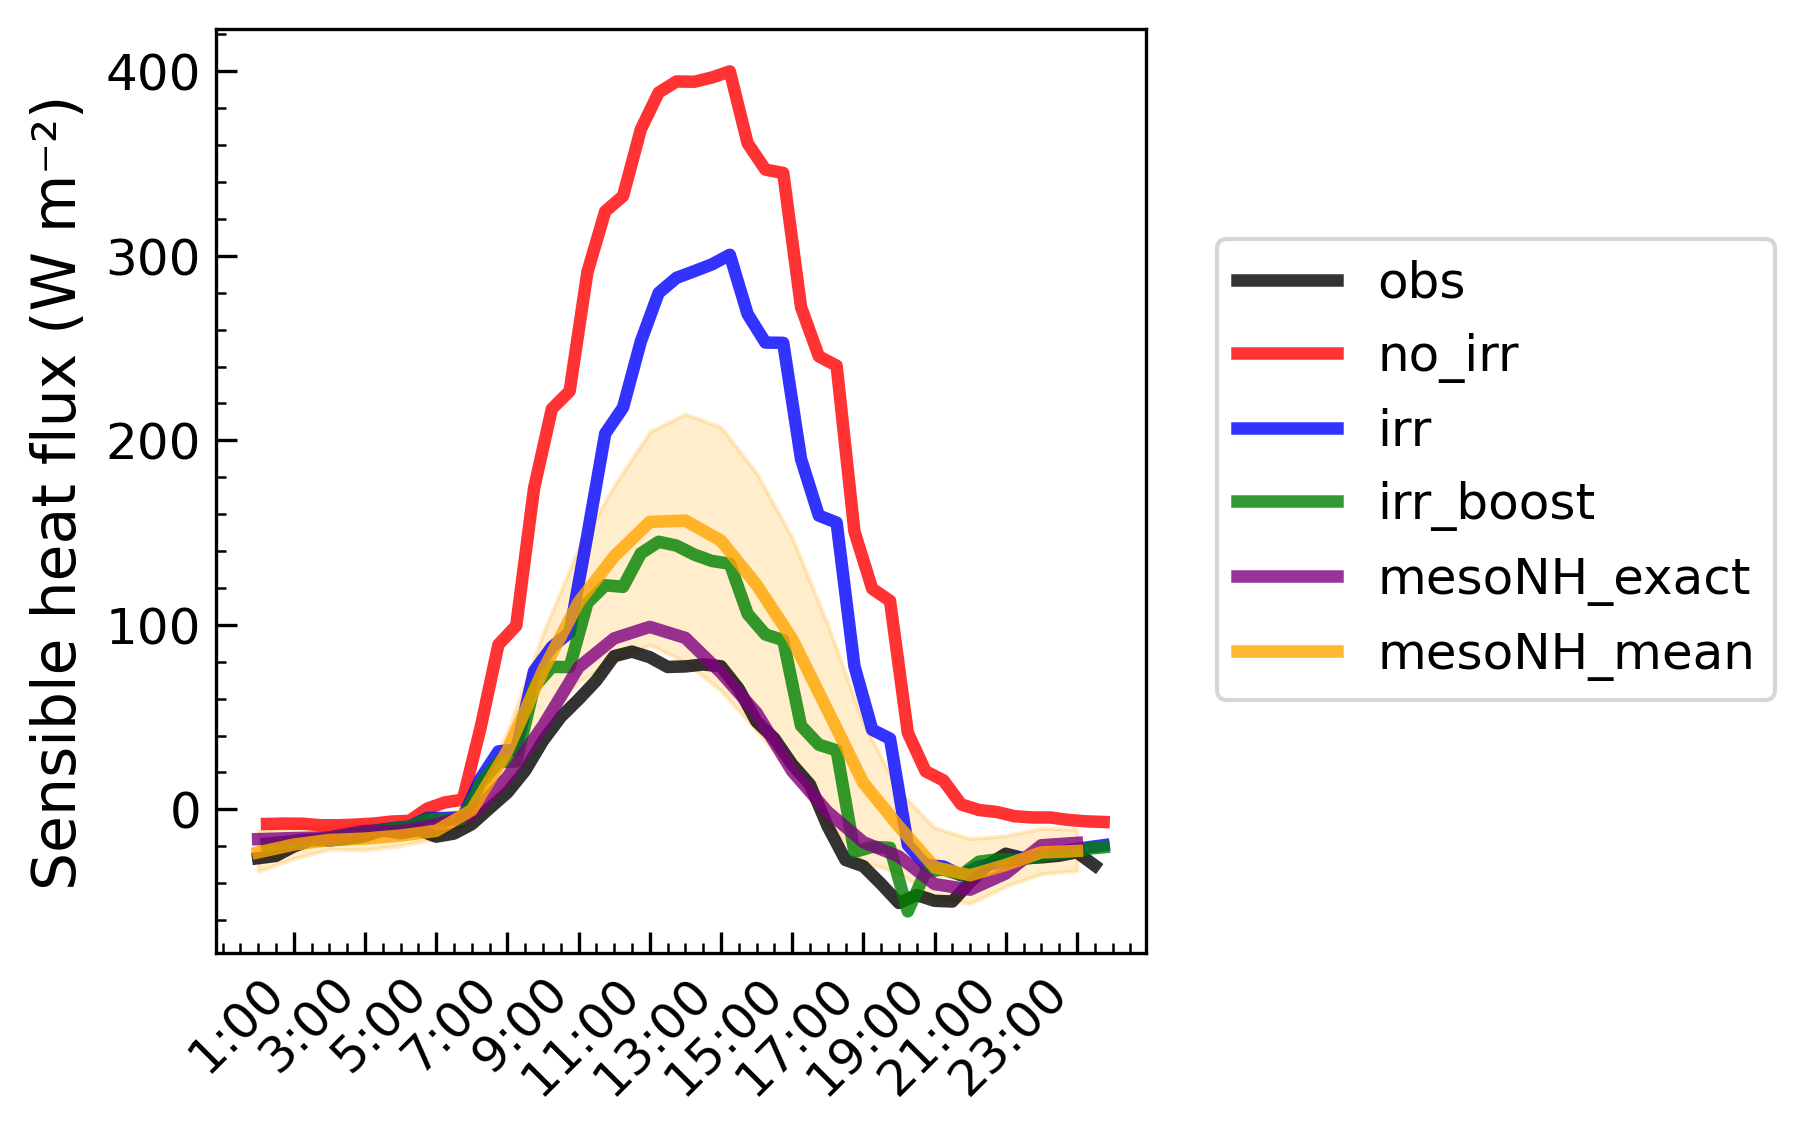
\includegraphics[width=\textwidth]{images/chap5/SOP_TS_DC/diurnal_cycle_cendrosa_sens.png}
        \end{subfigure} \\
        \begin{subfigure}[t]{0.5\textwidth}
            \caption{}
            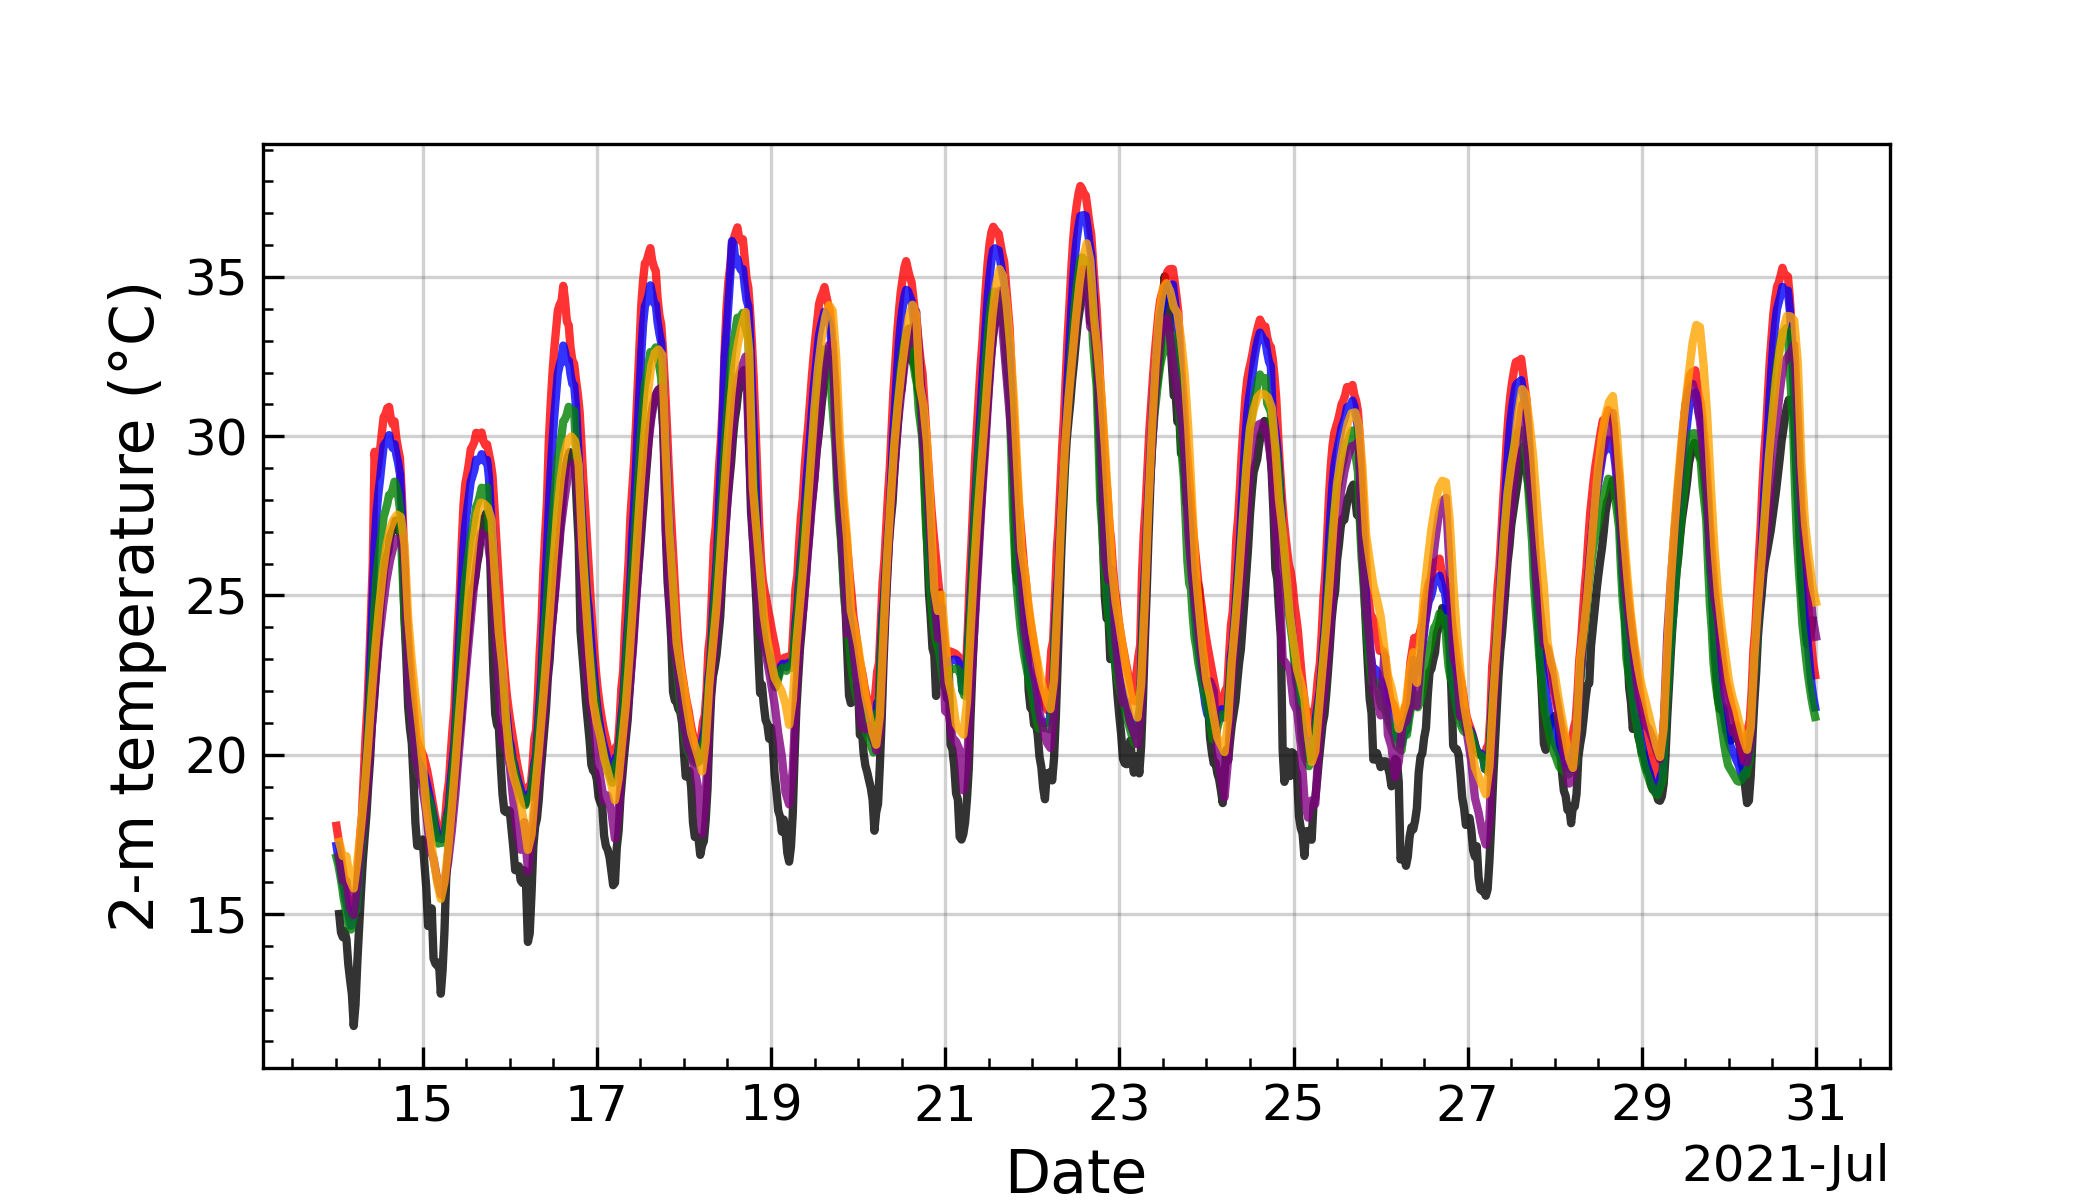
\includegraphics[width=\textwidth]{images/chap5/SOP_TS_DC/time_series_cendrosa_t2m.png}
        \end{subfigure} &
        \begin{subfigure}[t]{0.5\textwidth}
            \caption{}
            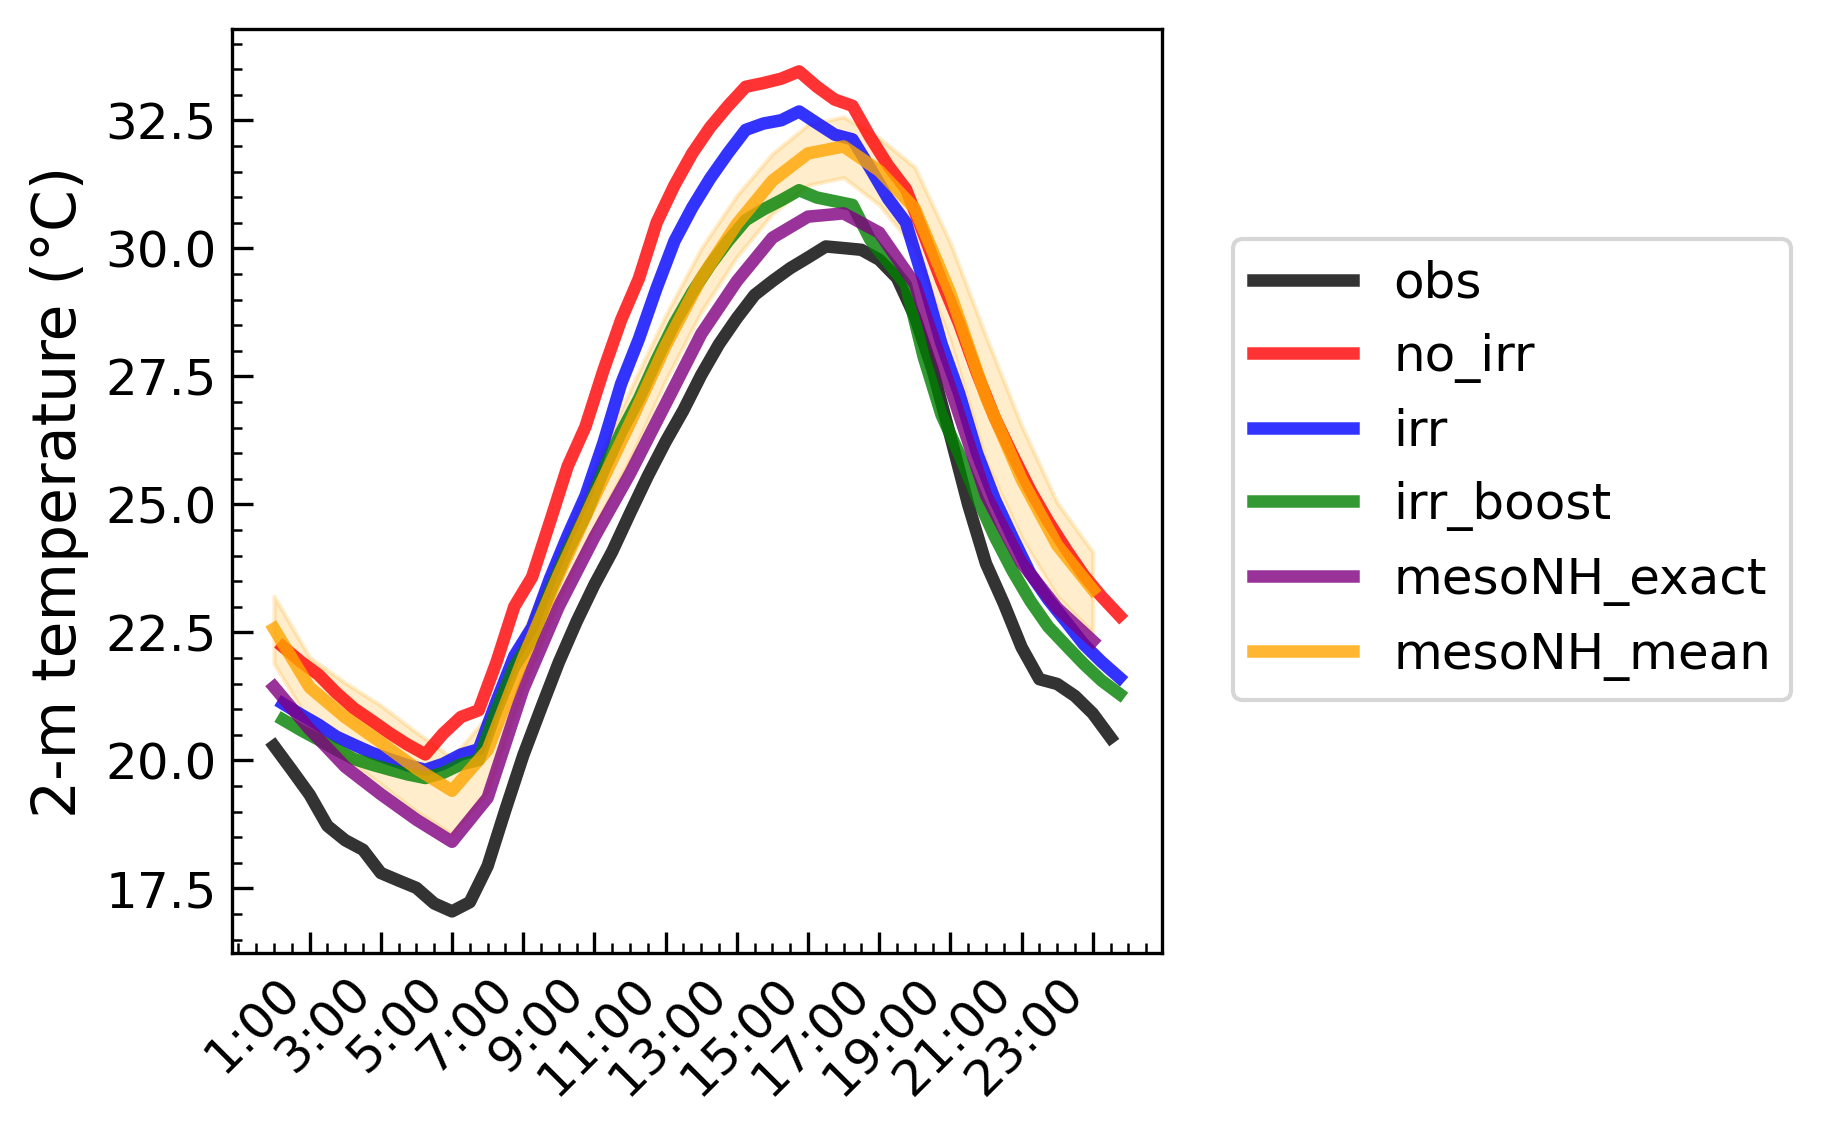
\includegraphics[width=\textwidth]{images/chap5/SOP_TS_DC/diurnal_cycle_cendrosa_t2m.png}
        \end{subfigure} \\
        \begin{subfigure}[t]{0.5\textwidth}
            \caption{}
            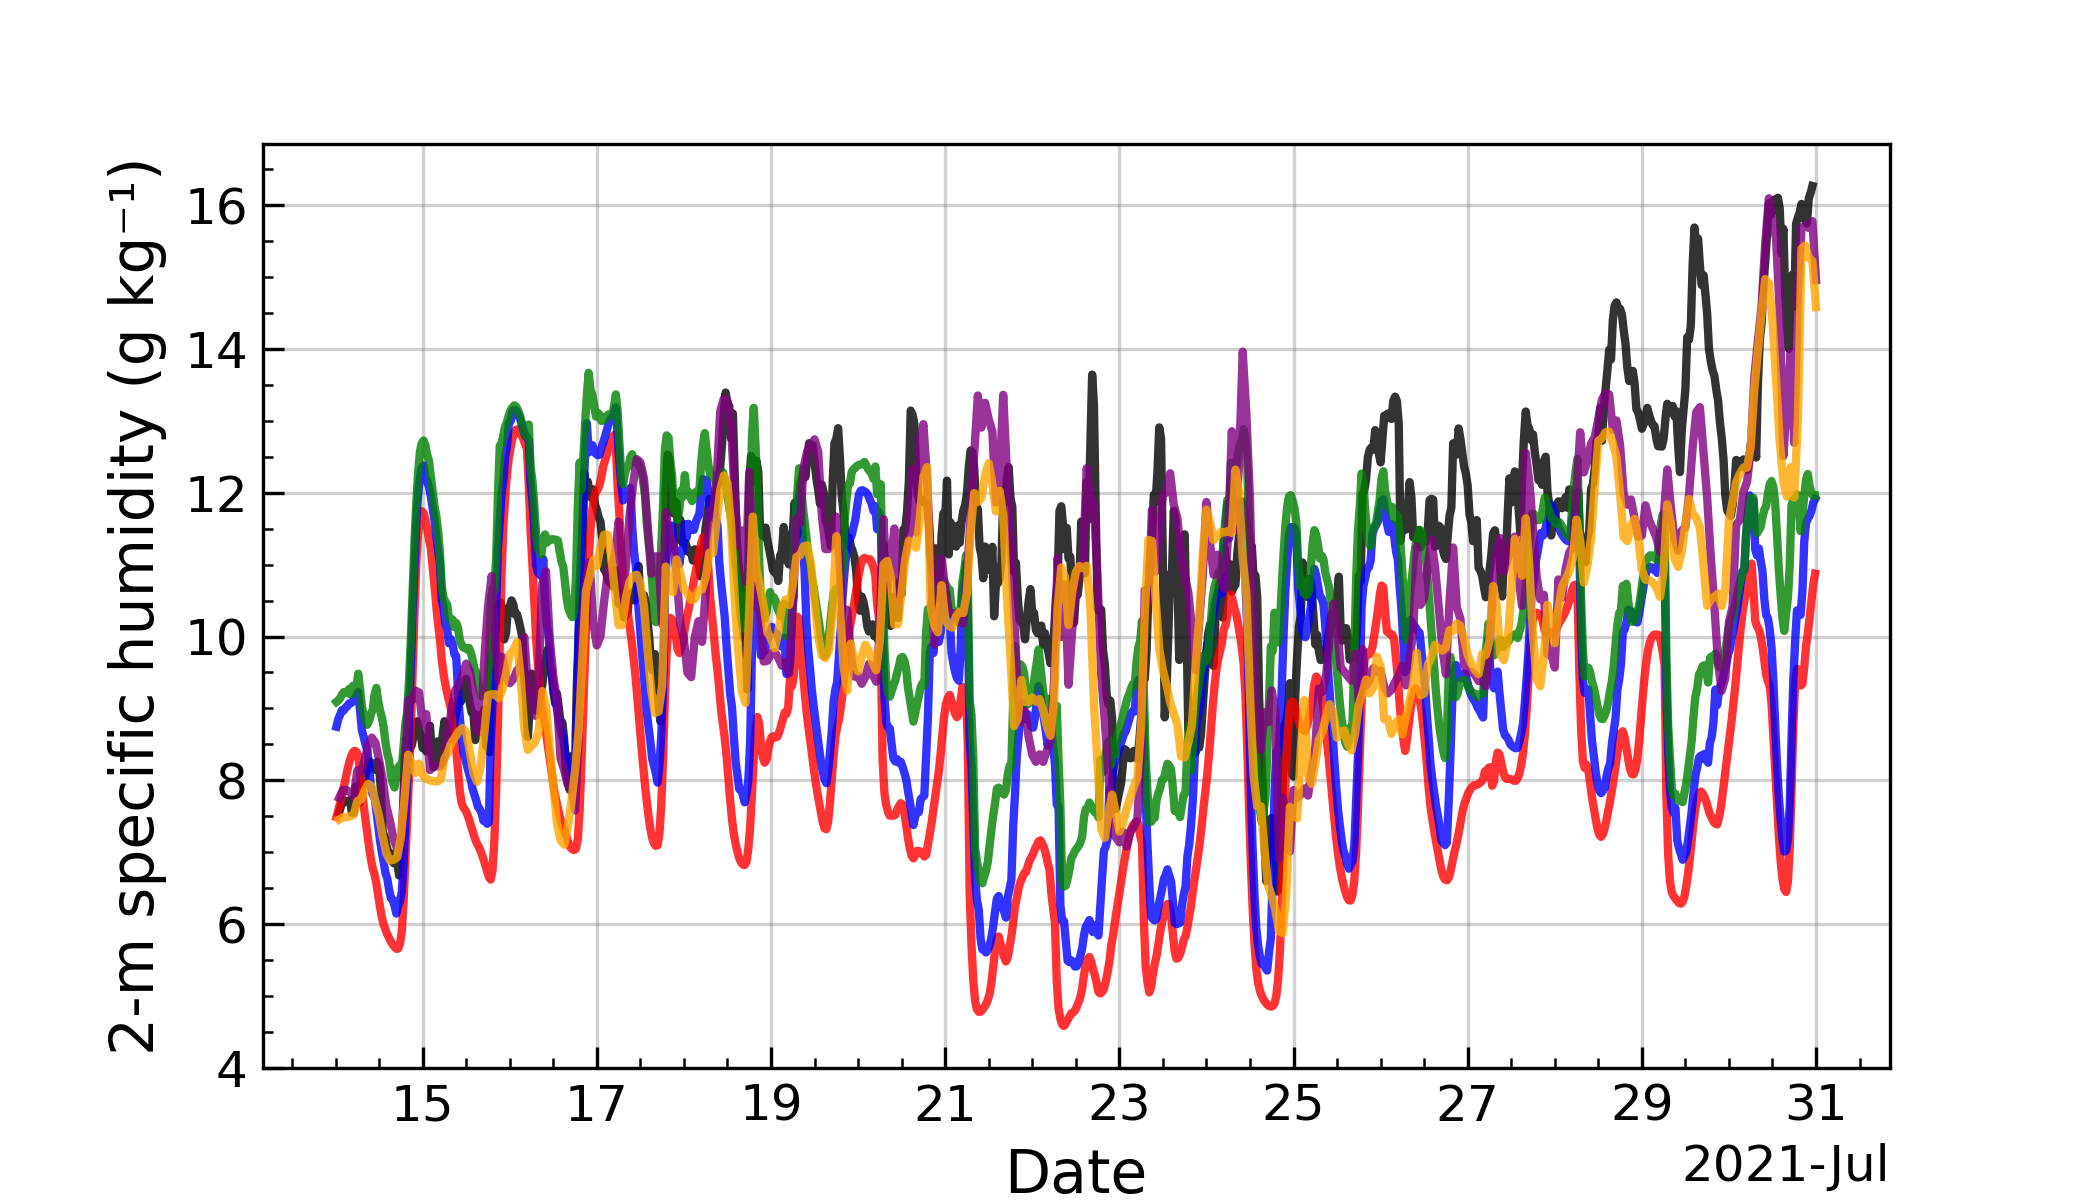
\includegraphics[width=\textwidth]{images/chap5/SOP_TS_DC/time_series_cendrosa_q2m.png}
        \end{subfigure} &
        \begin{subfigure}[t]{0.5\textwidth}
            \caption{}
            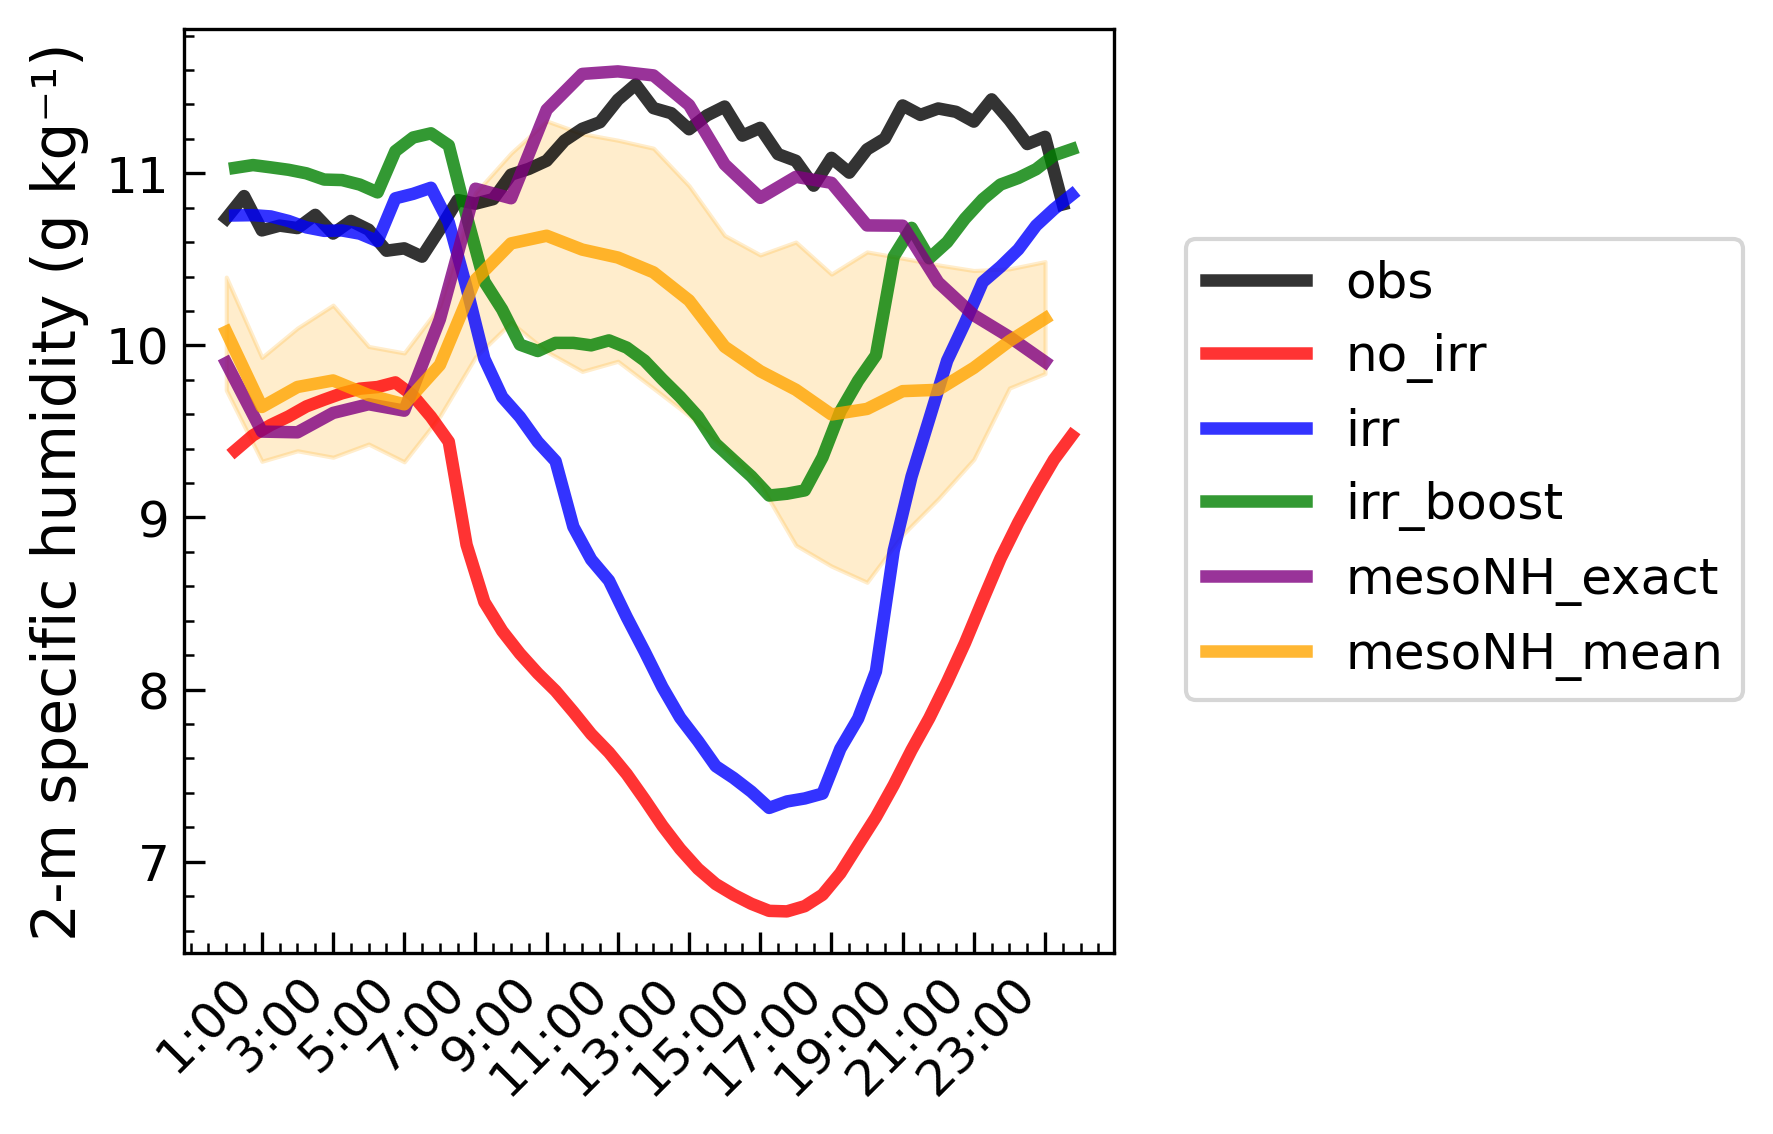
\includegraphics[width=\textwidth]{images/chap5/SOP_TS_DC/diurnal_cycle_cendrosa_q2m.png}
        \end{subfigure}
    \end{tabular}
    \caption{Time series and mean diurnal cycle of surface turbulent fluxes at La Cendrosa (irrigated site), 14-30 July 2021. The envelope for \mesomean represents the 25th and 75th percentiles of the distribution.}
    \label{fig:cendrosa_surfacevars}
\end{figure}


%Fig : Wind on both sites
\begin{figure}[hbtp]
    \centering
    \begin{tabular}{cc}
        \begin{subfigure}[t]{0.5\textwidth}
            \caption{}
            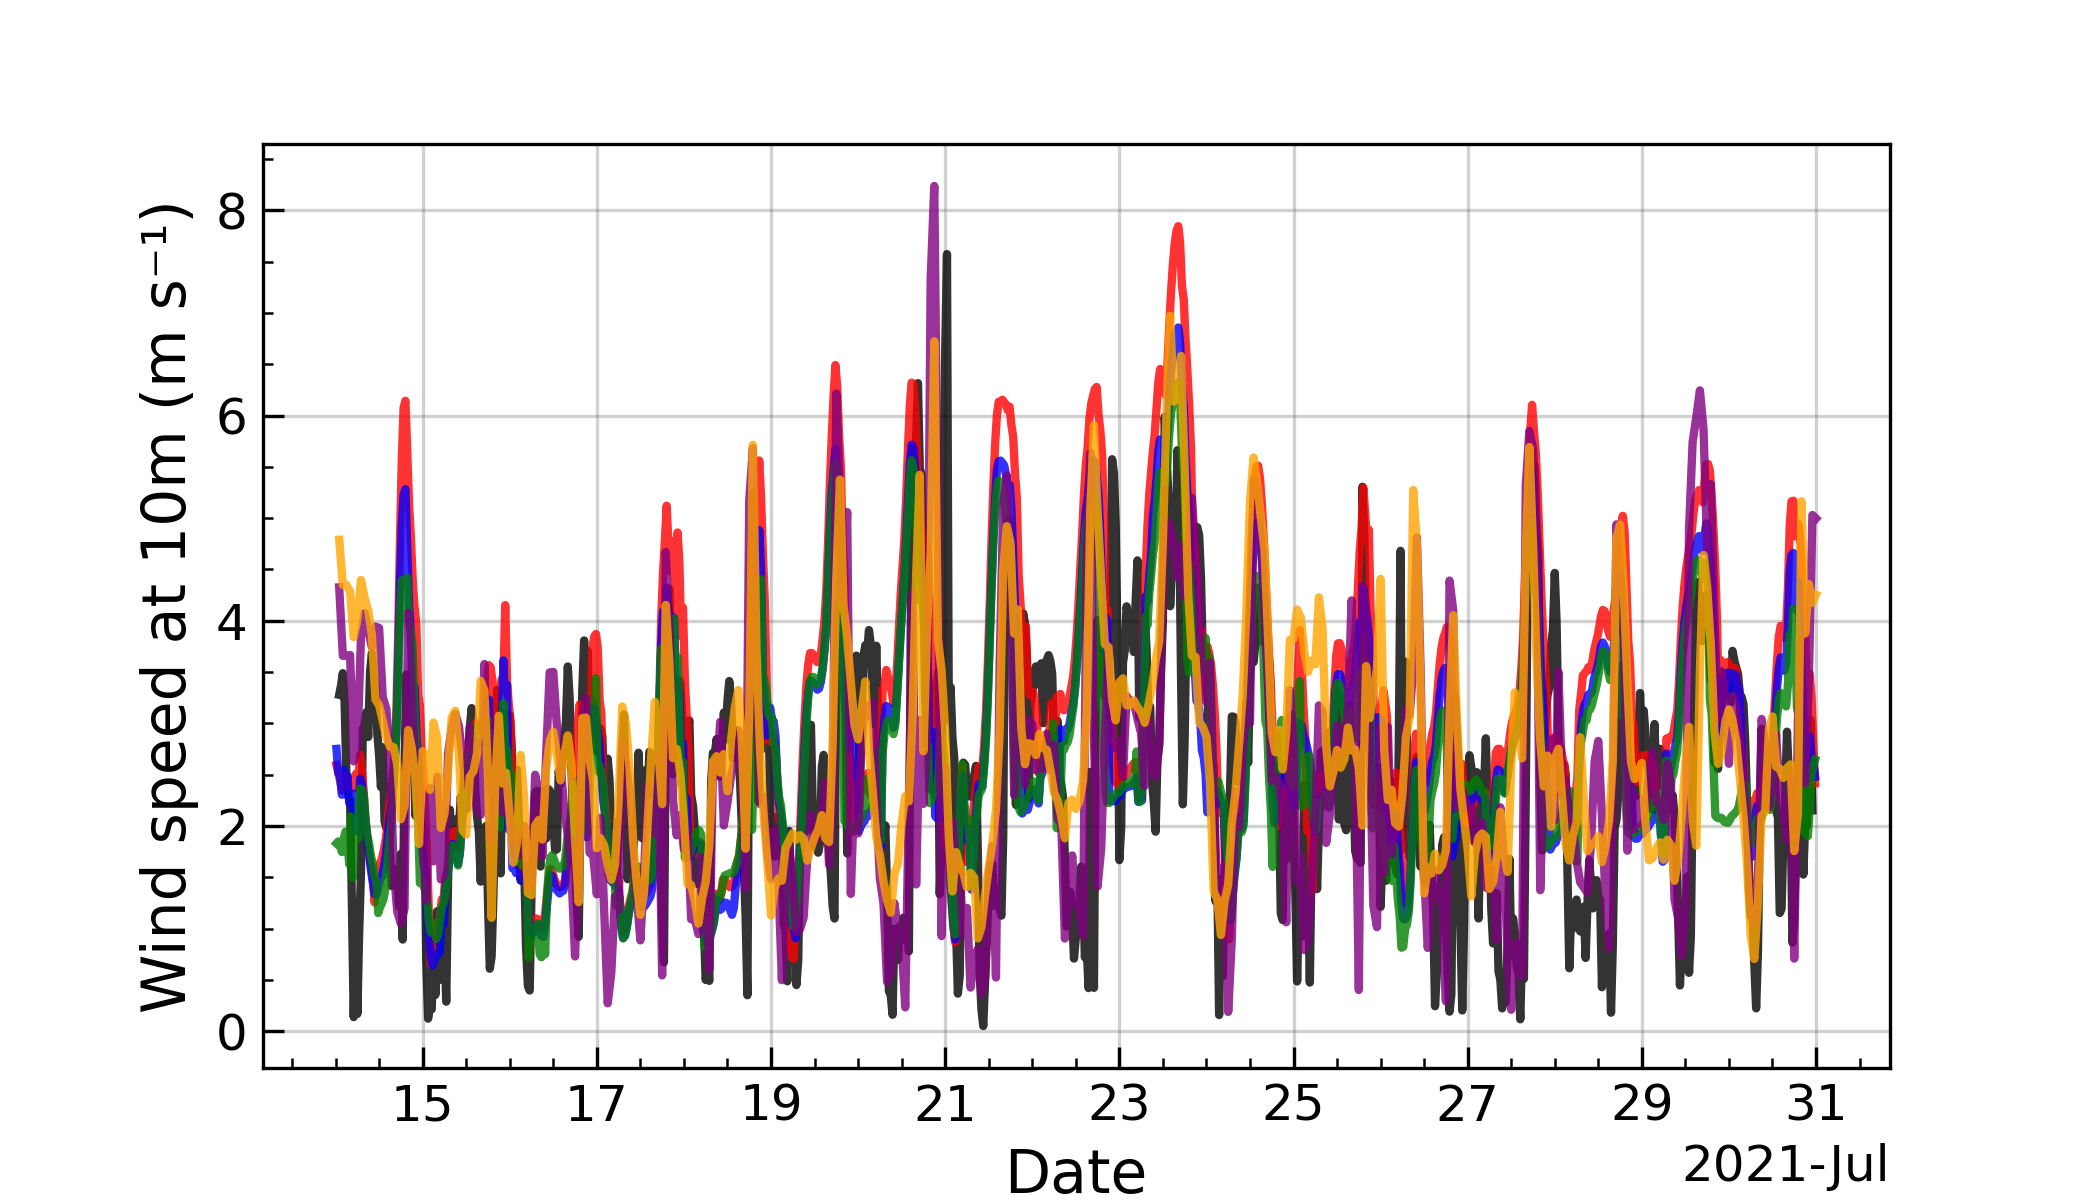
\includegraphics[width=\textwidth]{images/chap5/SOP_TS_DC/time_series_cendrosa_wind_speed_10m.png}
        \end{subfigure} &
        \begin{subfigure}[t]{0.5\textwidth}
            \caption{}
            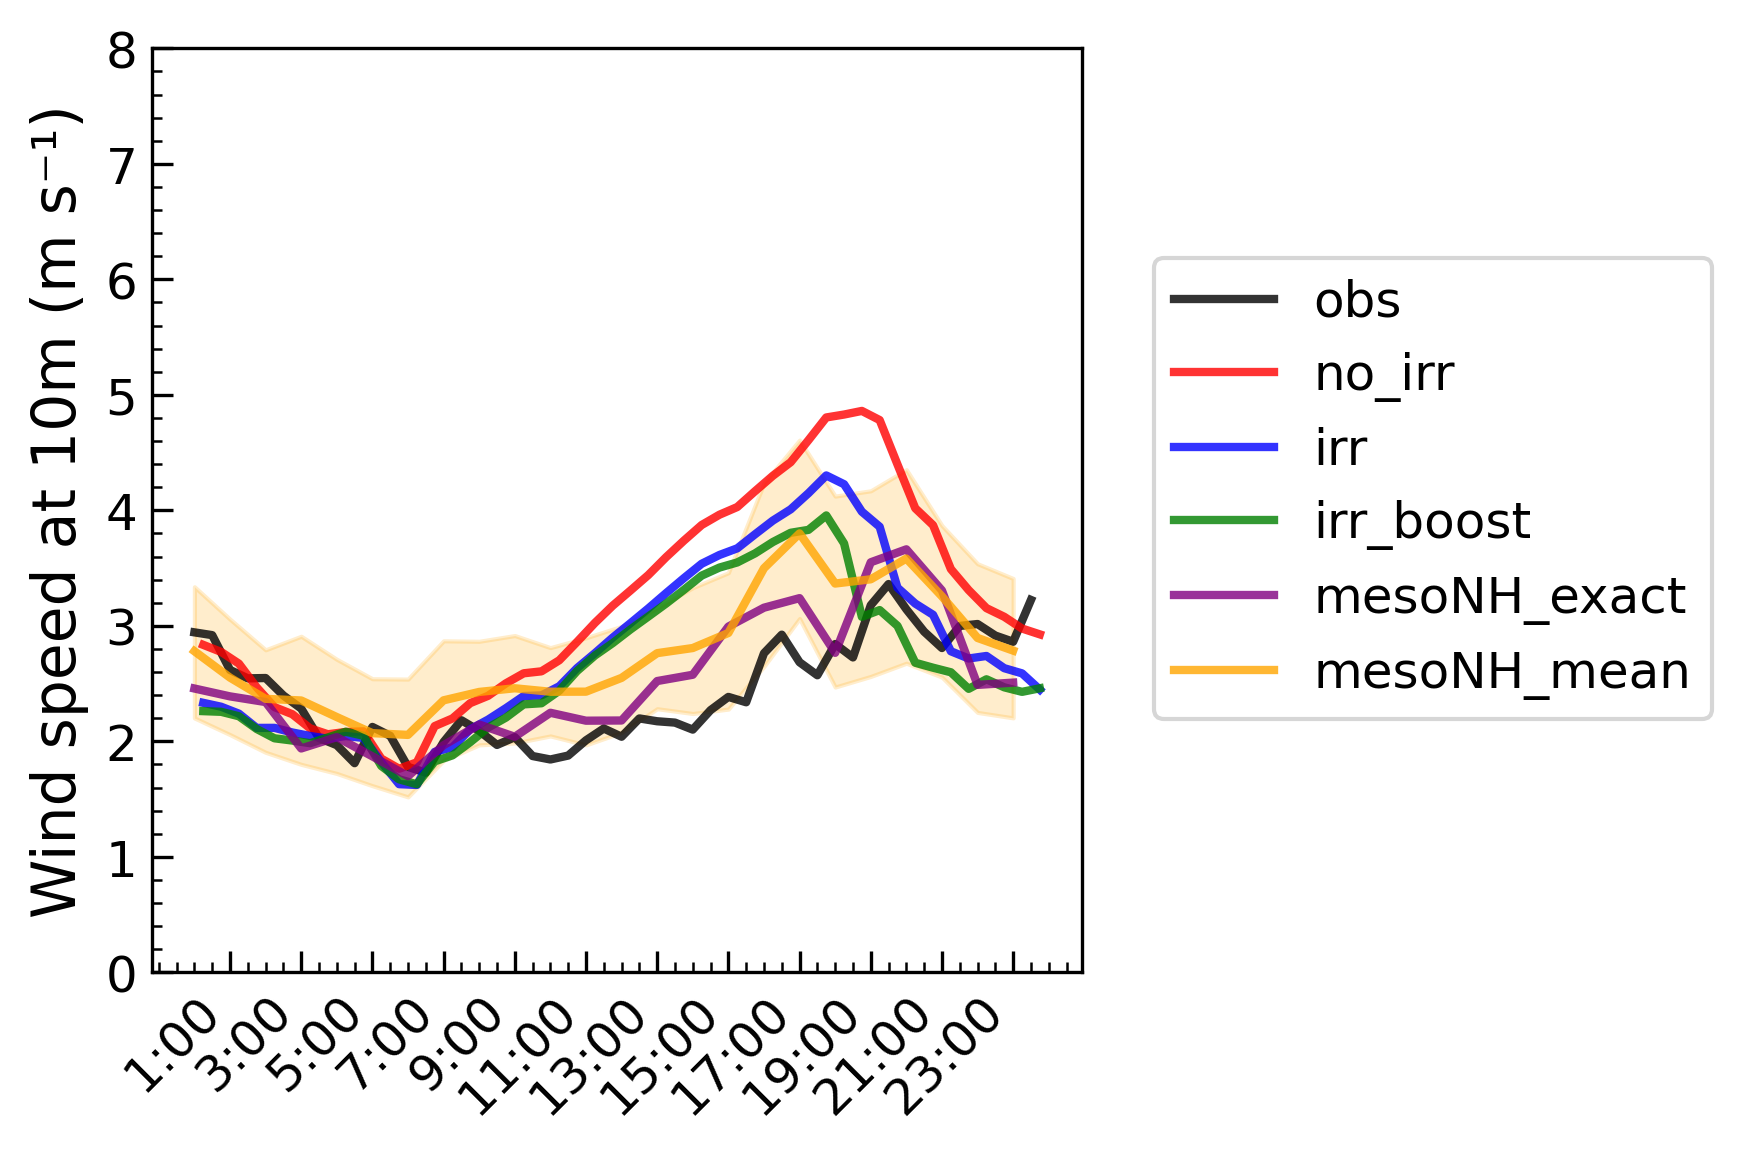
\includegraphics[width=\textwidth]{images/chap5/SOP_TS_DC/diurnal_cycle_cendrosa_wind_speed_10m.png}
        \end{subfigure} \\
        \begin{subfigure}[t]{0.5\textwidth}
            \caption{}
            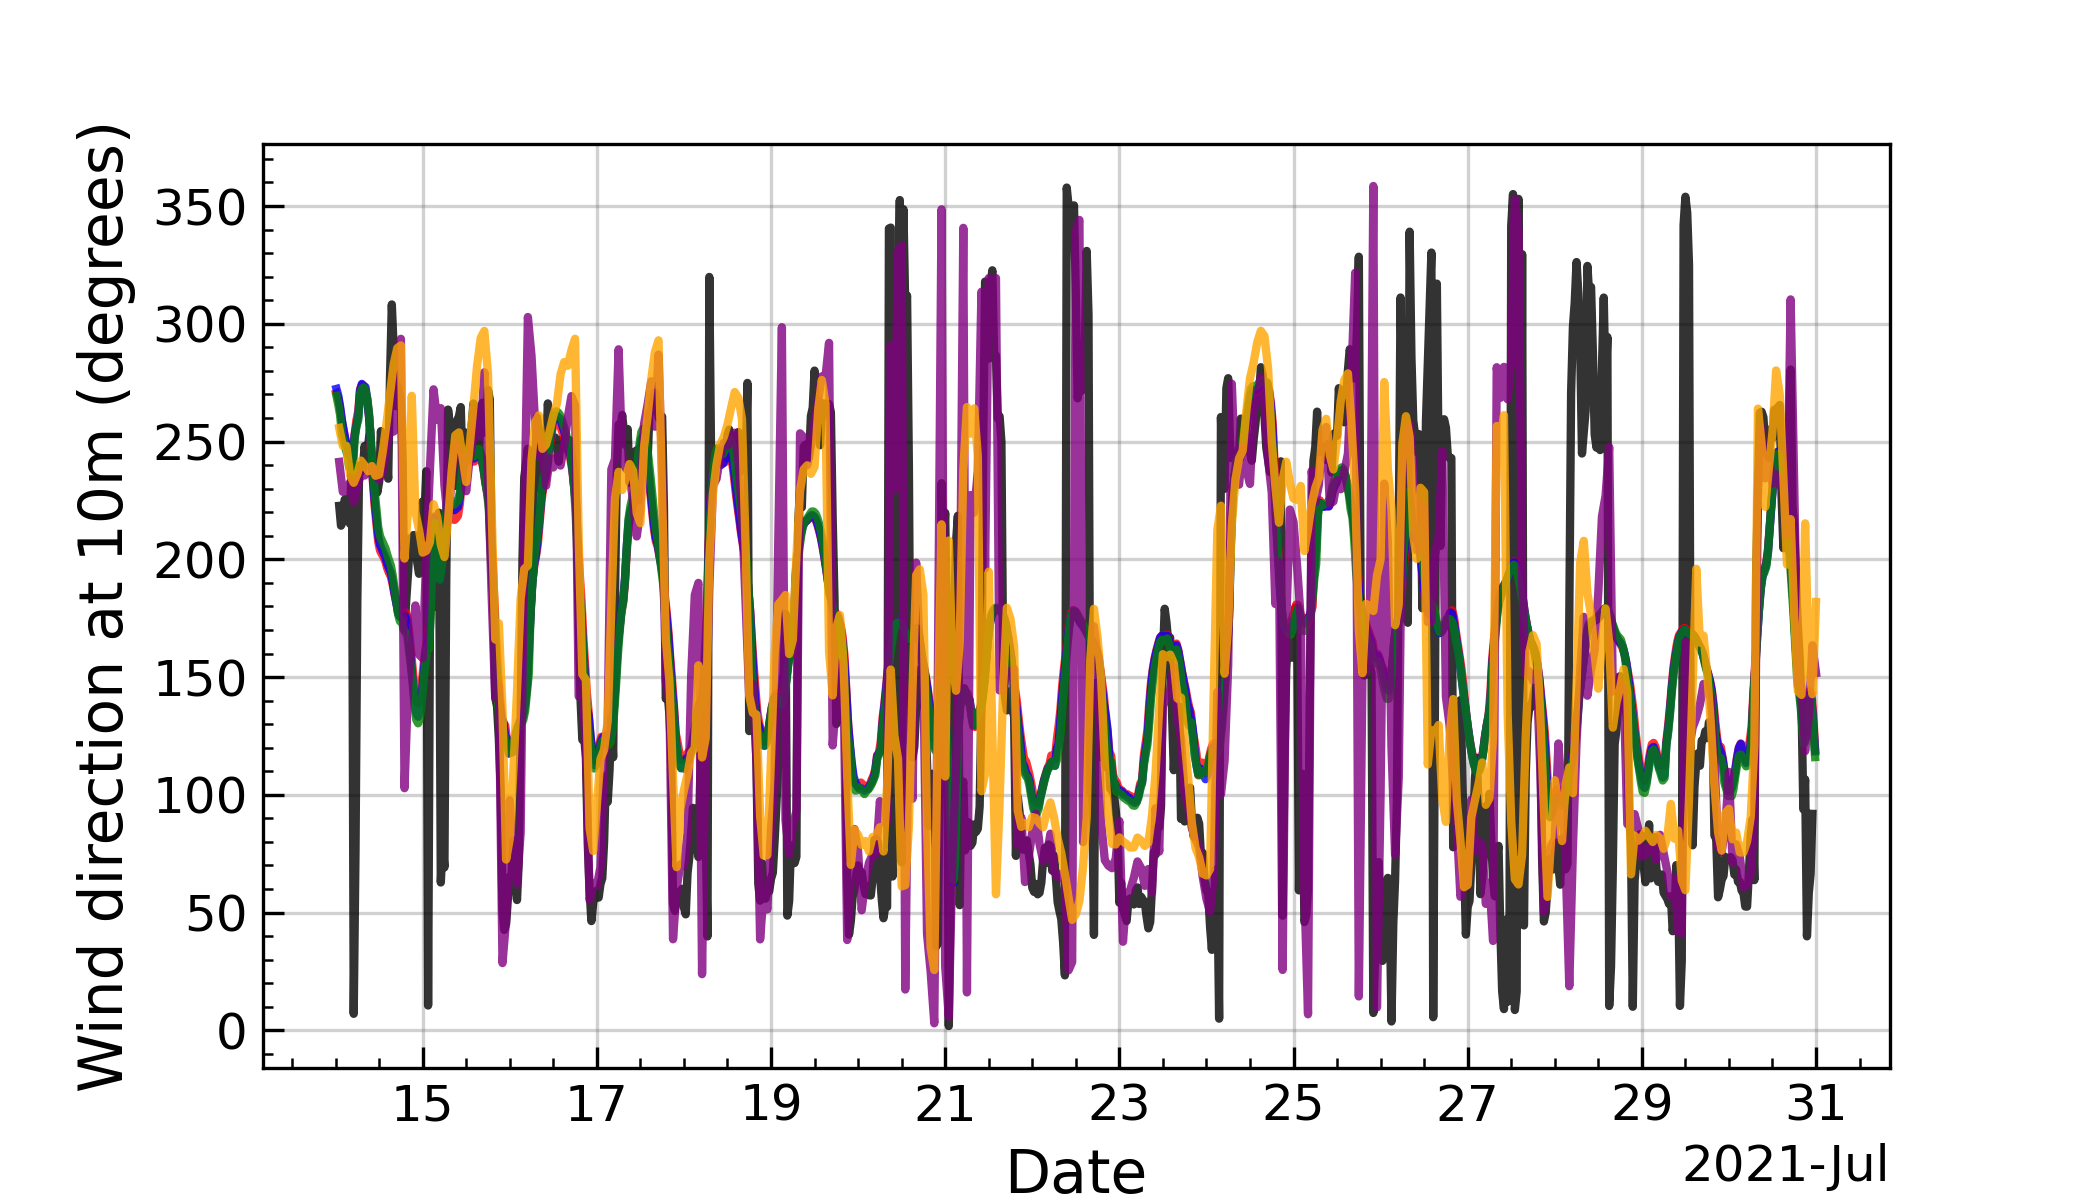
\includegraphics[width=\textwidth]{images/chap5/SOP_TS_DC/time_series_cendrosa_wind_direction_10m.png}
        \end{subfigure} &
        \begin{subfigure}[t]{0.5\textwidth}
            \caption{}
            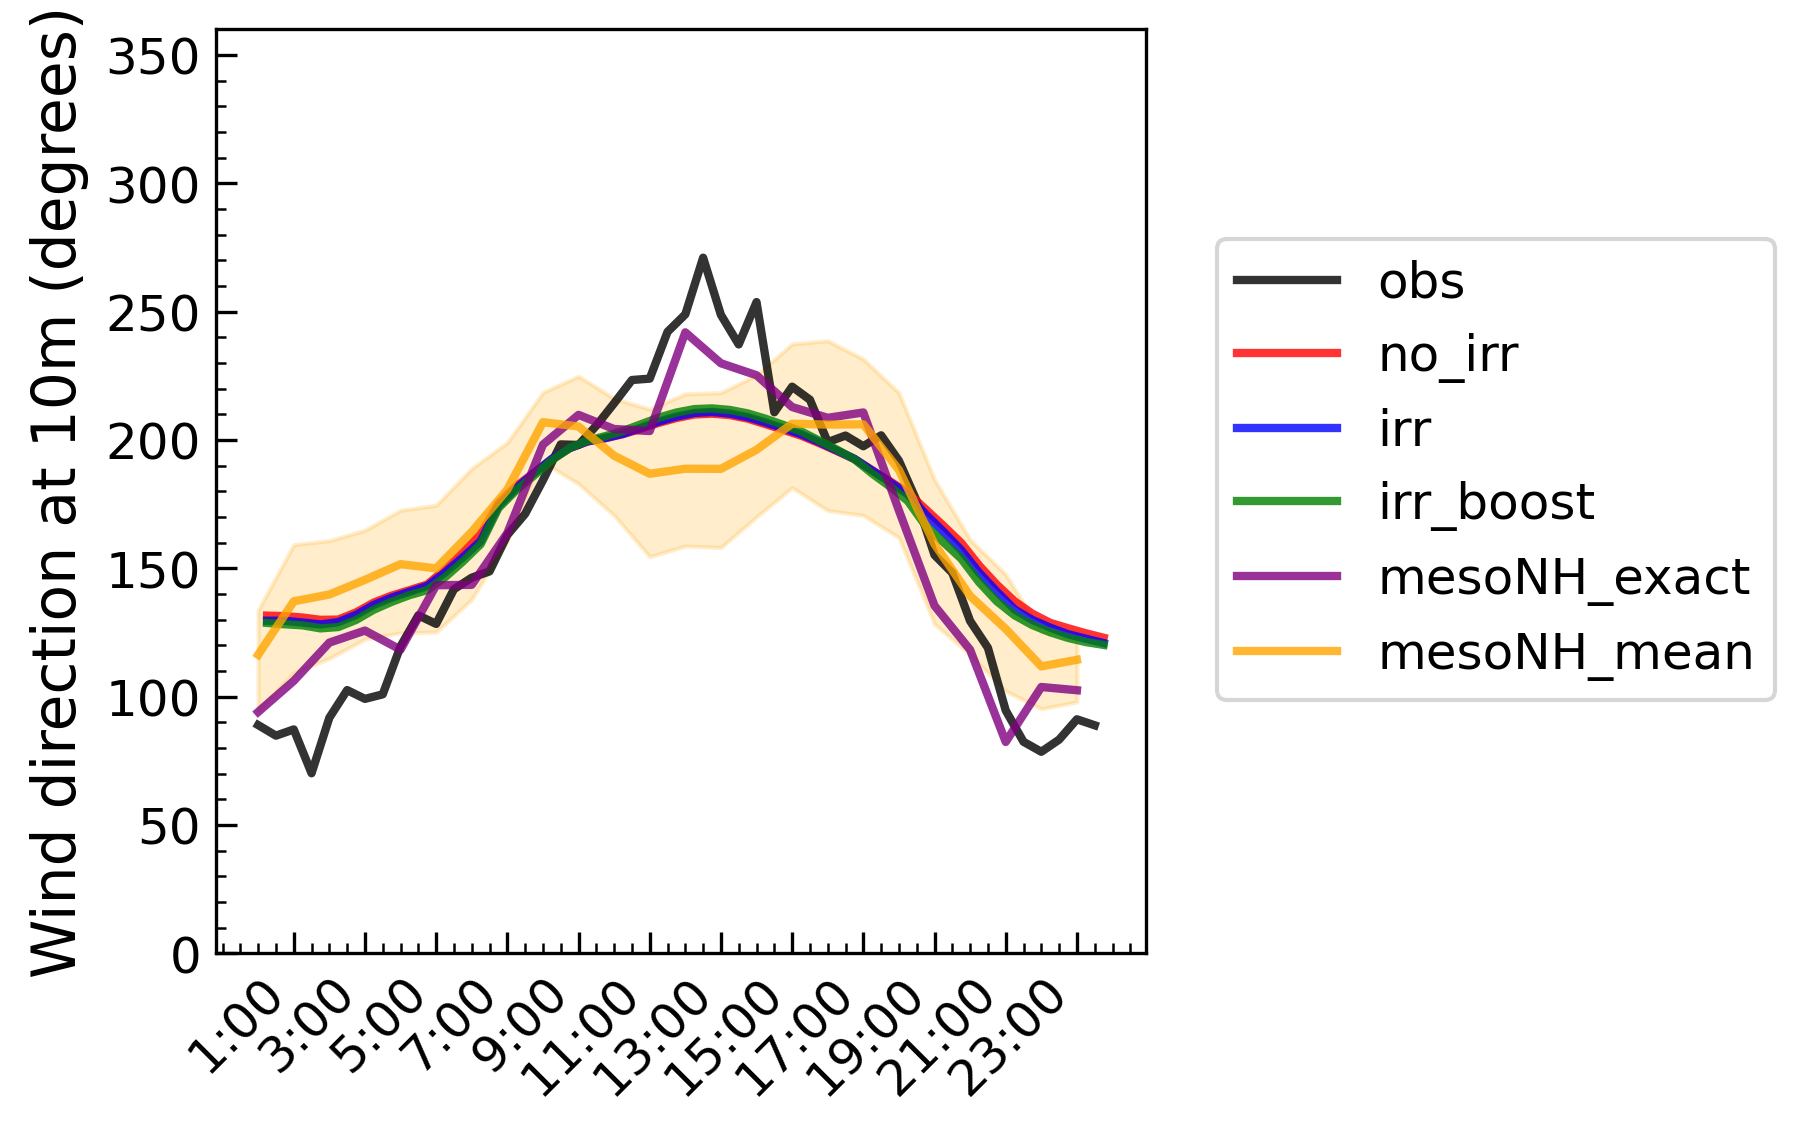
\includegraphics[width=\textwidth]{images/chap5/SOP_TS_DC/diurnal_cycle_cendrosa_wind_direction_10m.png}
        \end{subfigure} \\
        \begin{subfigure}[t]{0.5\textwidth}
            \caption{}
            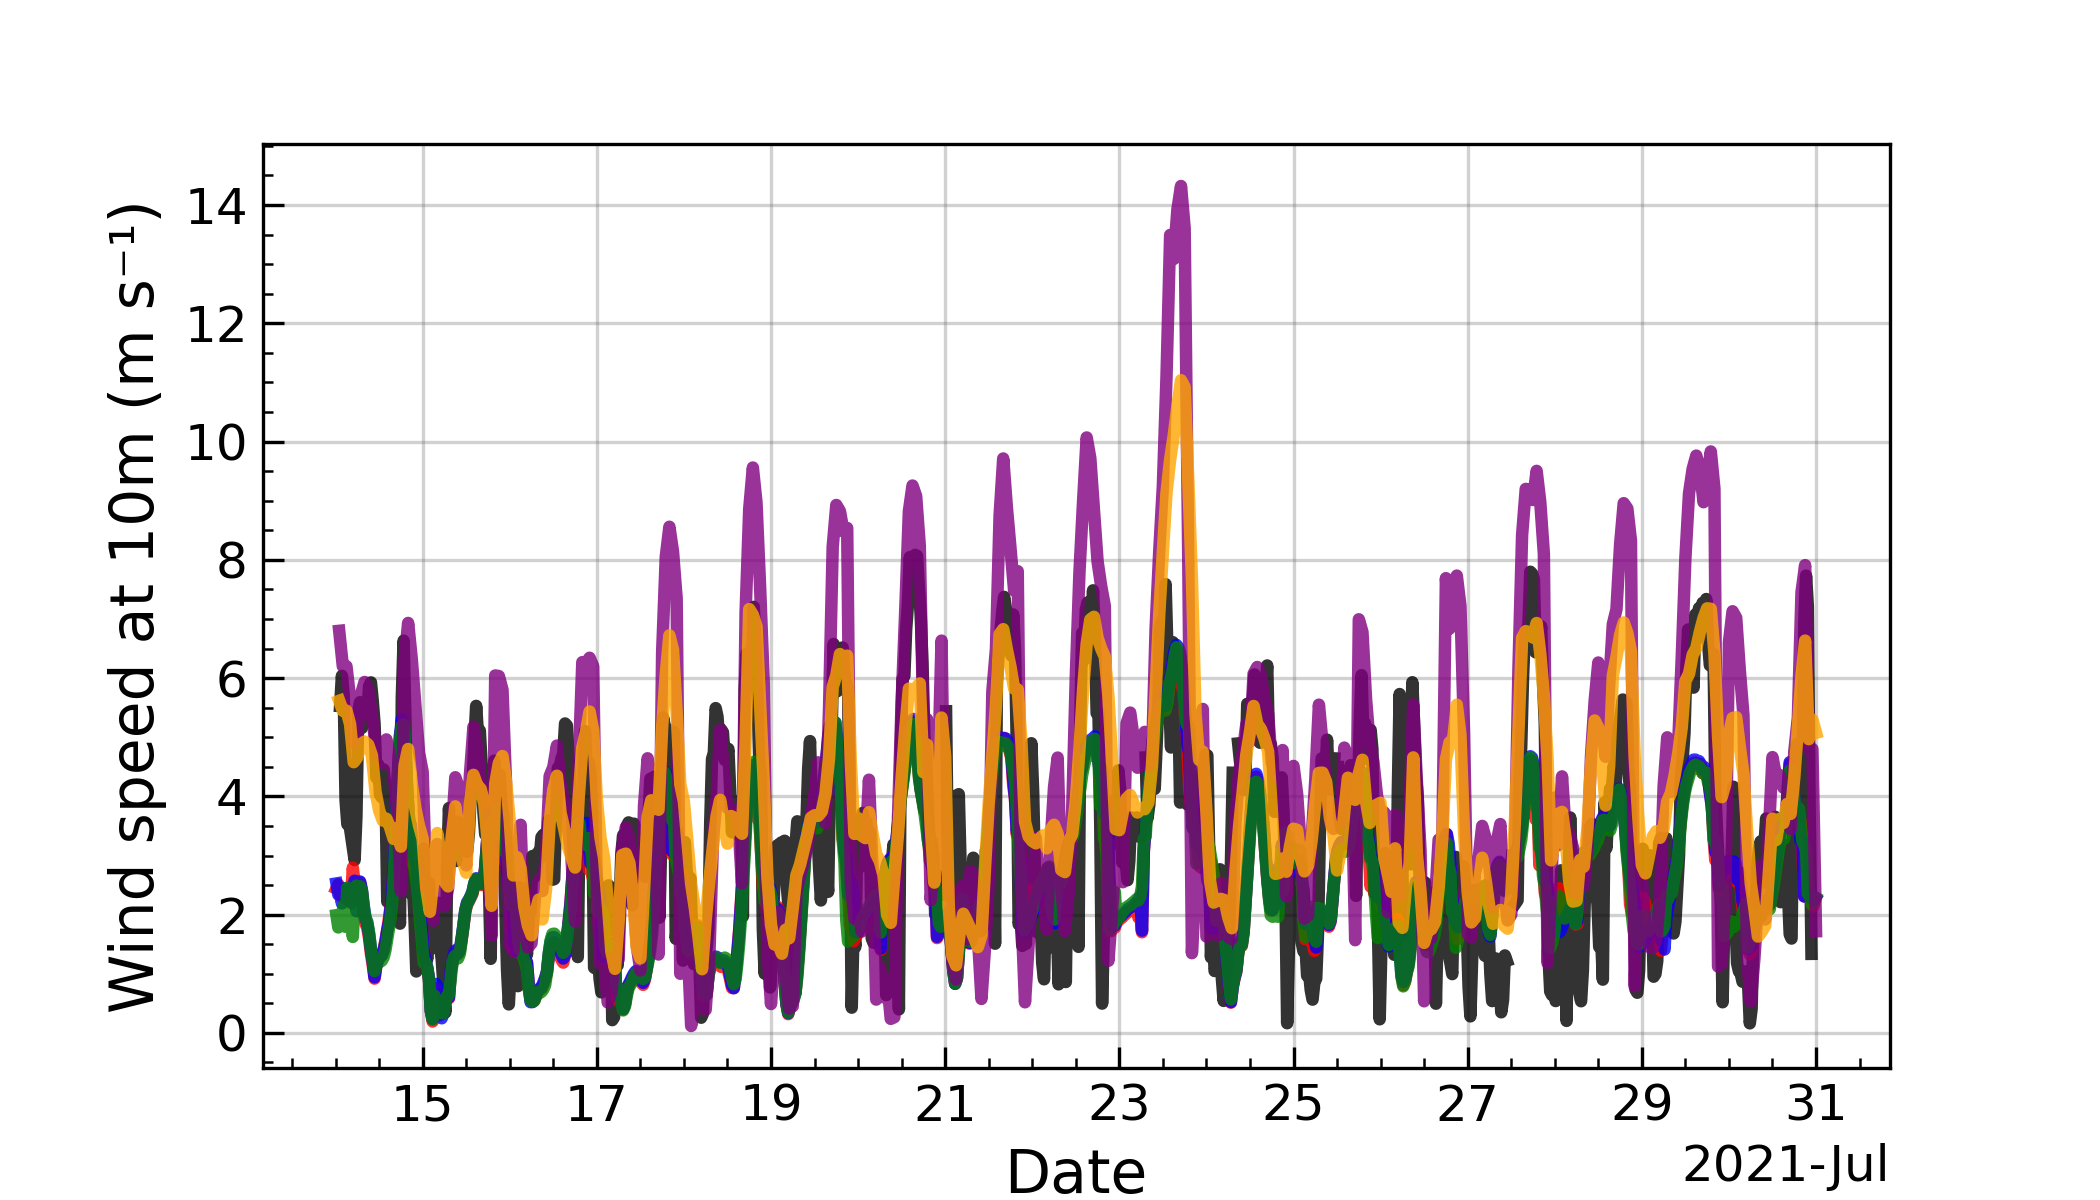
\includegraphics[width=\textwidth]{images/chap5/SOP_TS_DC/time_series_elsplans_wind_speed_10m.png}
        \end{subfigure} &
        \begin{subfigure}[t]{0.5\textwidth}
            \caption{}
            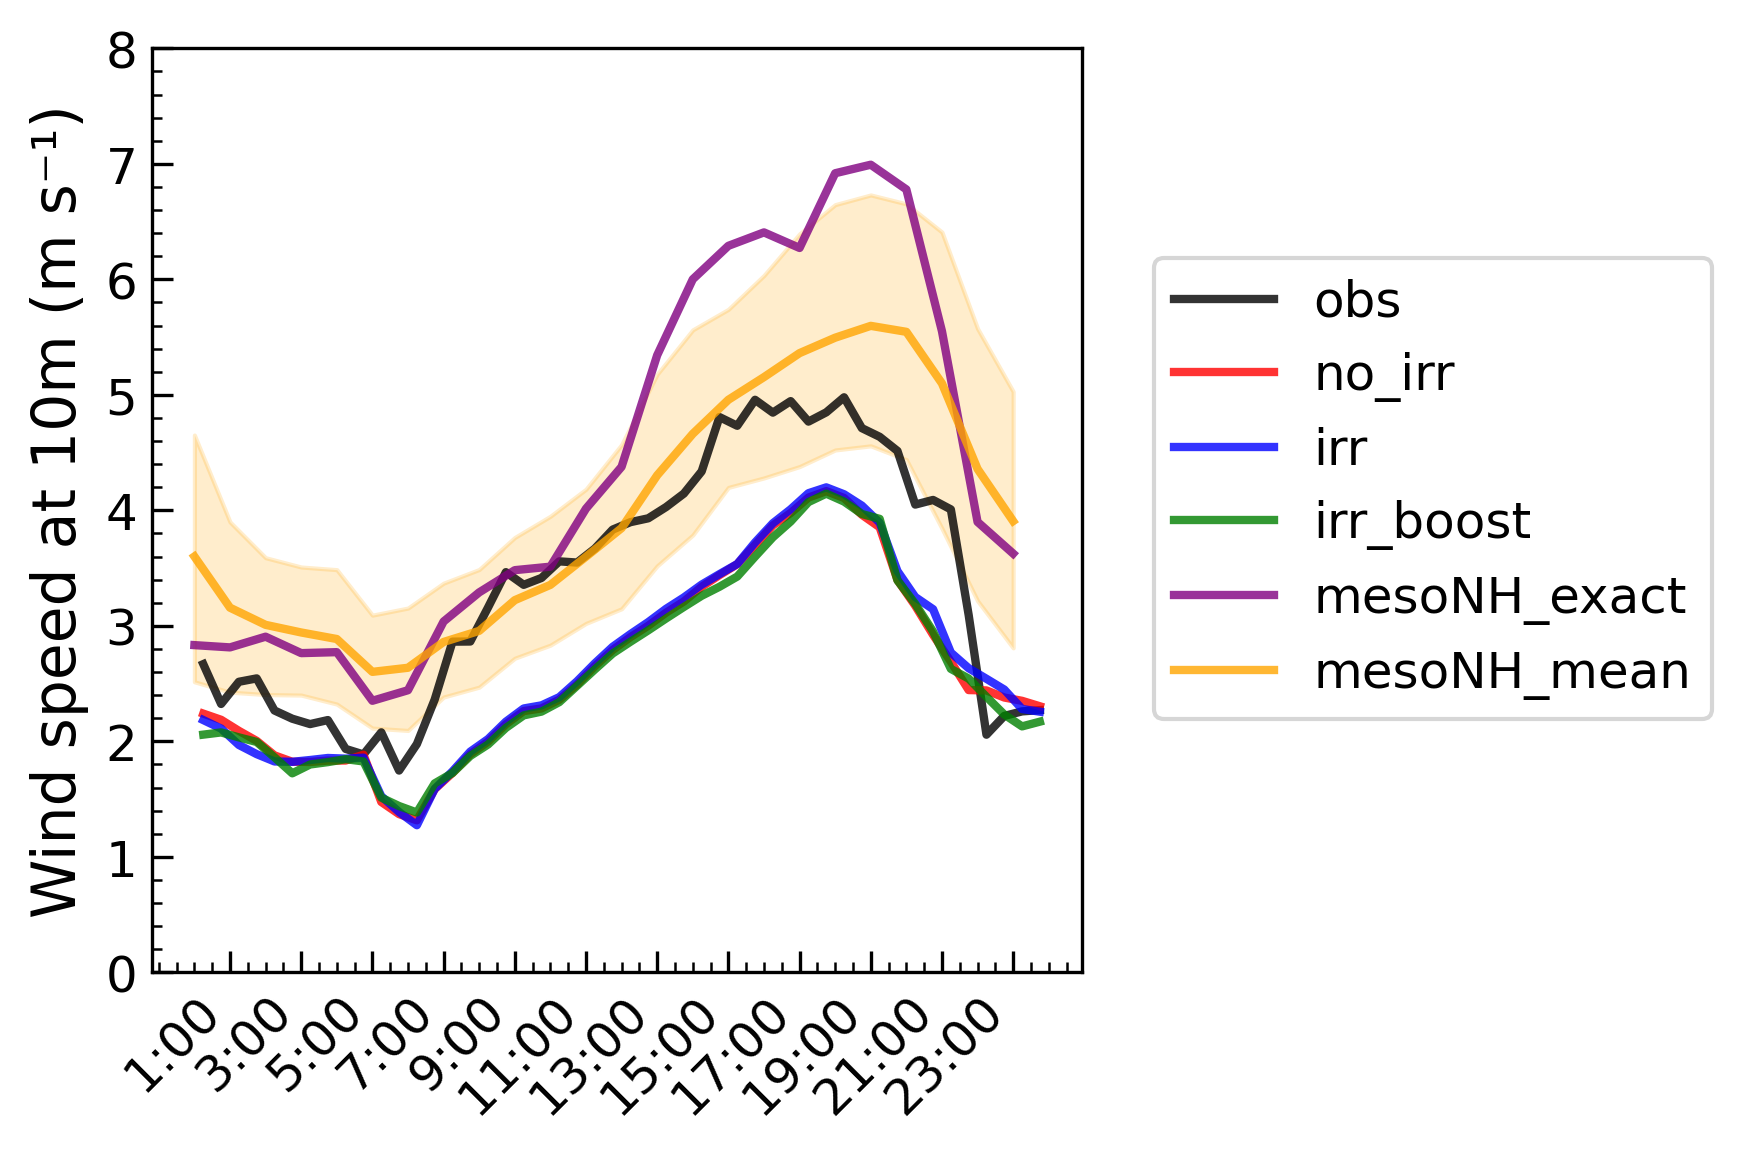
\includegraphics[width=\textwidth]{images/chap5/SOP_TS_DC/diurnal_cycle_elsplans_wind_speed_10m.png}
        \end{subfigure} \\
        \begin{subfigure}[t]{0.5\textwidth}
            \caption{}
            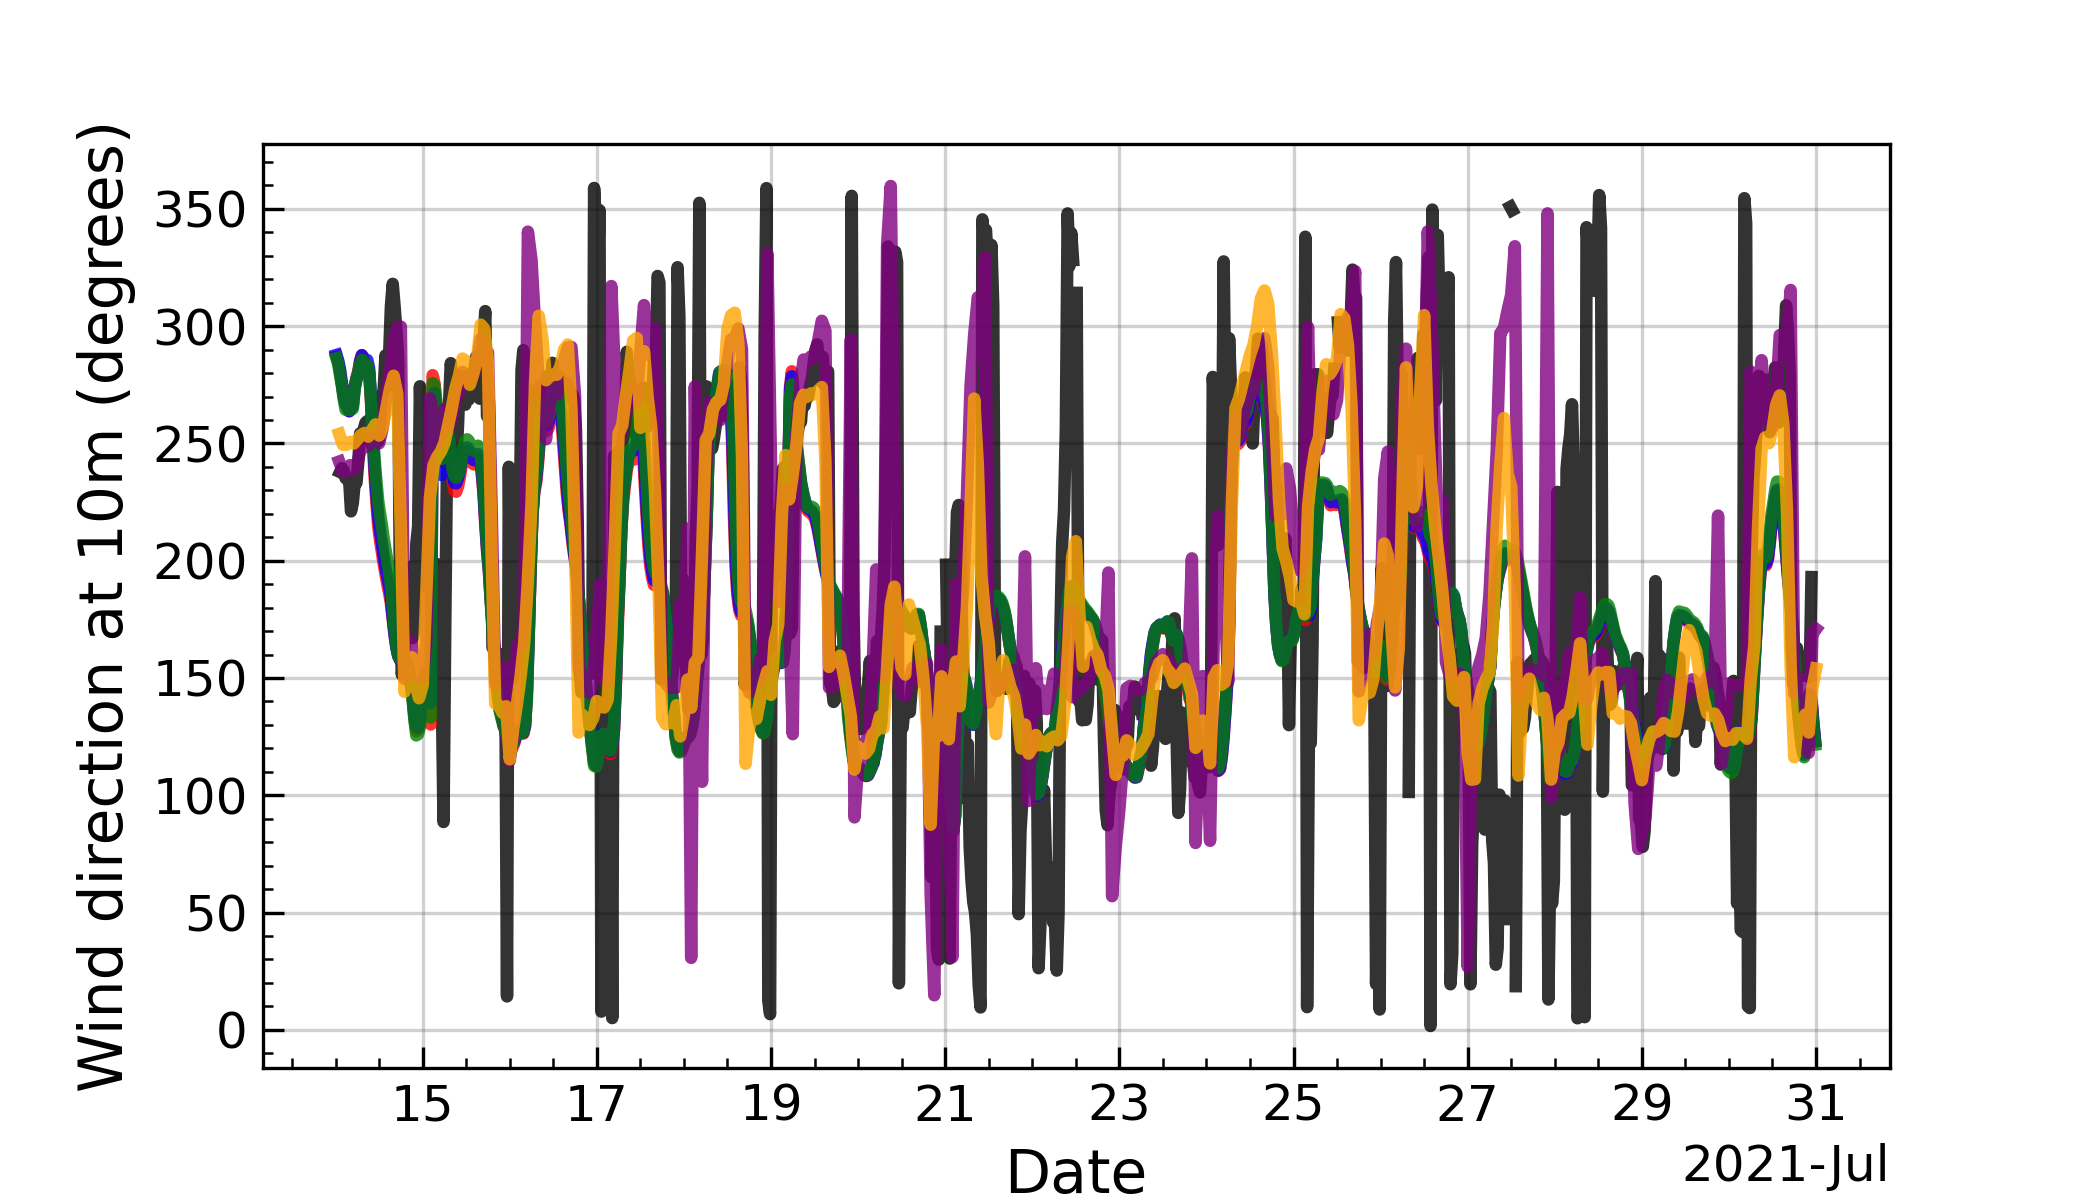
\includegraphics[width=\textwidth]{images/chap5/SOP_TS_DC/time_series_elsplans_wind_direction_10m.png}
        \end{subfigure} &
        \begin{subfigure}[t]{0.5\textwidth}
            \caption{}
            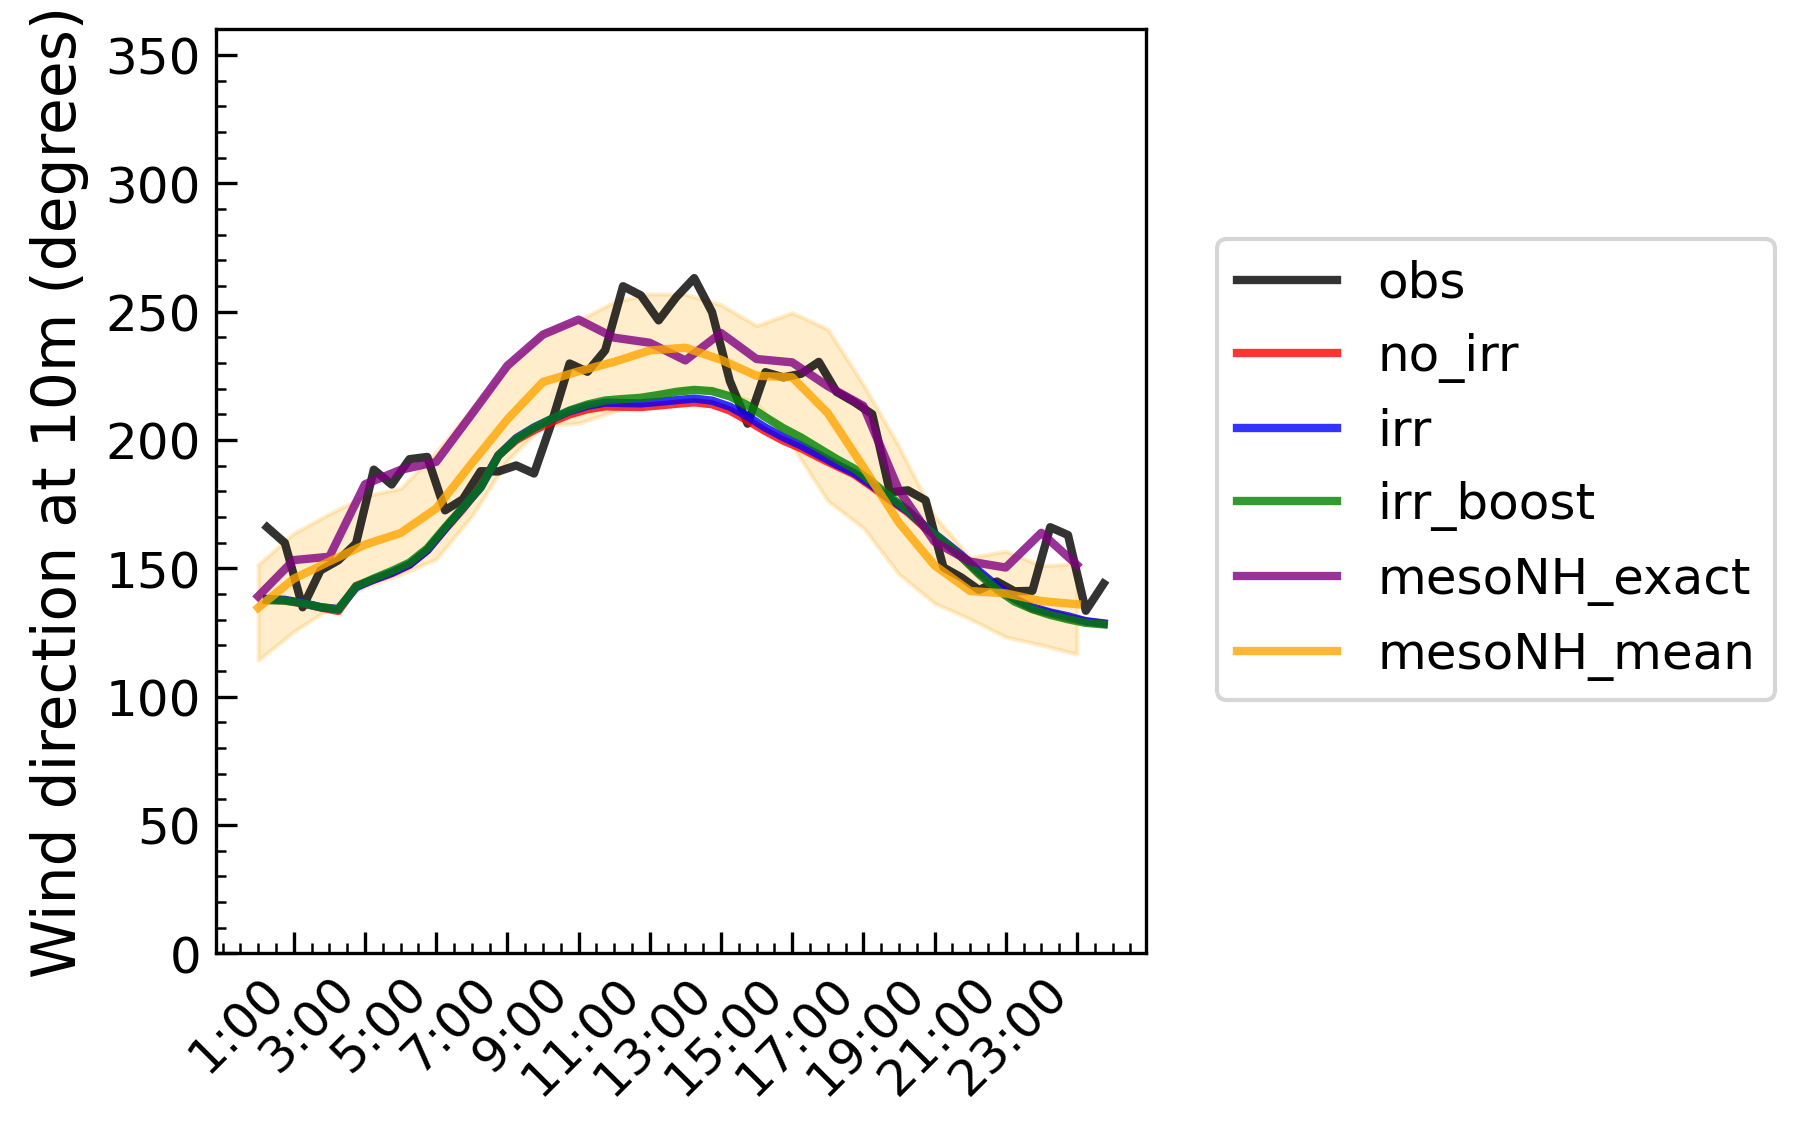
\includegraphics[width=\textwidth]{images/chap5/SOP_TS_DC/diurnal_cycle_elsplans_wind_direction_10m.png}
        \end{subfigure}
    \end{tabular}
    \caption{Time series and mean diurnal cycle of wind speed and direction on both sites, 14-30 July 2021. The envelope for \mesomean represents the 25th and 75th percentiles of the distribution.}
    \label{fig:bothsites_wind}
\end{figure}

\hfill

%%ELS PLANS%%
Looking into near-surface conditions at the Els Plans site (Fig. \ref{fig:elsplans_surfacevars}) serves as a useful comparison to assess the general performance of both models in a context that is largely independent of soil moisture.
The energy partitioning between turbulent fluxes is very different, since the average observed latent heat flux is below 20 W \persqm while the sensible heat flux is three times larger than at La Cendrosa (Fig. \ref{fig:elsplans_surfacevars}b, d). 
The three ICOLMDZ simulations are very similar and the lines for \noirr and \irr completely overlap, while latent heat flux is slightly increased (5-10 W \persqm) in \irrboost since ORCHIDEE still computes a small irrigation for this grid cell. 
%option:explain the details ? Demand is 0 but then interpolated to DEM, satisfied on some grid cells near the border of the hexagon and reinterpolated to ORC heaxagonal grid.
ICOLMDZOR underestimates the already weak latent heat flux and overestimates the sensible heat flux with a peak value higher than 400 W \persqm whereas the observed one is around 300 W \persqm. 
Regarding the Meso-NH simulation, the \mesoexact diurnal cycle of latent heat flux looks a bit different from the observed one, with a higher and sharper peak around 12UTC instead of the smooth shape seen in observations. The diurnal cycle of sensible heat flux matches the observed shape but presents an overestimation from 11UTC until the evening.
The latent heat flux of \mesomean is clearly driven by the few irrigated grid cells that fall into the hexagon (Fig. \ref{fig:liaise_sites_grid_cells}c), leading the mean value to exceed the 75th percentile. These outliers have much less influence on the sensible heat flux which shows a smaller spread and is even closer to observations than \mesoexact.
On the contrary to La Cendrosa, it was not really expected to see the \irr or \irrboost simulation matching \mesomean because the input map of irrigated fraction was voluntarily modified to limit irrigation on this grid cell. This was done with the initial objectives of creating a constrated situation compared to La Cendrosa and achieving a better match with on-site observations, but clearly made the comparison of grid-cell average fluxes less relevant.
%option:add that no big reservoir here so no irrigation at all if not cheating ? (and too much if cheating ?)

The average diurnal cycle of 2-meter temperature (Fig. \ref{fig:elsplans_surfacevars}f) confirms the presence of a warm bias in Meso-NH at night (more than 2°C), and shows a slight underestimation of the peak value in the afternoon. 
%option: further links to fsens, LWup, Tsurf ?
%NB : sur les deux sites, LWdn est sous estimé de ~15W/m² en journée par les deux modèles (sauf \noirr sur La Cendrosa car air plus chaud), probablement ce qui permet d'être bon sur fsens alors que flat est surestimé (manque d'énergie incidente donc pas de compensation parfaite entre les deux)
It also highlights the very good performance of ICOLMDZOR on this non-irrigated site, although the peak is slightly too early compared to the observed one, as also seen at La Cendrosa.
The observed evolution of 2-meter specific humidity over the day is very different from La Cendrosa, since it is highest at night and steadliy decreases throughout the day with a minimal peak at 16UTC on average over the SOP (Fig. \ref{fig:elsplans_surfacevars}h).
As seen in La Cendrosa, Meso-NH exhibits a dry bias at night but simulates correct humidity in the day. 
The diurnal evolution simulated by ICOLMDZOR is quite similar to the one at La Cendrosa, except that at Els Plans it is more in agreement with observations and Meso-NH. On average over the SOP, ICOLMDZOR strongly underestimates 2-meter specific humidity, but as visible in Fig. \ref{fig:elsplans_surfacevars}g, this is mostly due to the second part of the SOP where excessive drying occurs in all three ICOLMDZOR simulations. 
This supports the idea that the limitations in capturing near-surface humidity variations at La Cendrosa are mostly non-local and largely induced by large-scale advection. 
Finally, it can be noticed that irrigation has a visible impact on specific humidity, although not very large in comparison to the dry bias, also pointing to non-local effects on this variable since irrigation is very small on the Els Plans grid cell in ICOLMDOZOR.%todo:link to irrig TS

Observed wind speed at Els Plans is higher than at La Cendrosa (Fig. \ref{fig:bothsites_wind}f), which relflects the influence on roughness on a site with lower vegtation (Fig. \ref{fig:liaise_sites_photos}). On average, variations in direction are of smaller amplitude than at La Cendrosa (Fig. \ref{fig:bothsites_wind}h) but some quick regime changes can still be identified on most days (Fig. \ref{fig:bothsites_wind}g).
In ICOLMDZOR, the simulated wind speed and direction are very similar at Els Plans and La Cendrosa, which is not surprising since the grid cells are next to each other, but there are no more dfferences between the three simulations. This confirms the hypothesis that the wind speed differences at La Cendrosa were mainly the consequence of increased roughness in \irrboost and \irr. On average, ICOLMDZOR underestimates wind speed but reproduces the diurnal changes in wind direction. As seen at La Cendrosa, it captures the variations in wind direction much better in the beginning of the SOP than after the regime change on 20 July. On this second part of the SOP, a lot of regime changes are not represented by ICOLMDZOR and \mesomean, while only some of them are simulated in \mesoexact.

%Fig : Els Plans turbulent fluxes + t2m, q2m
\begin{figure}[hbtp]
    \centering
    \begin{tabular}{cc}
        \begin{subfigure}[t]{0.5\textwidth}
            \caption{}
            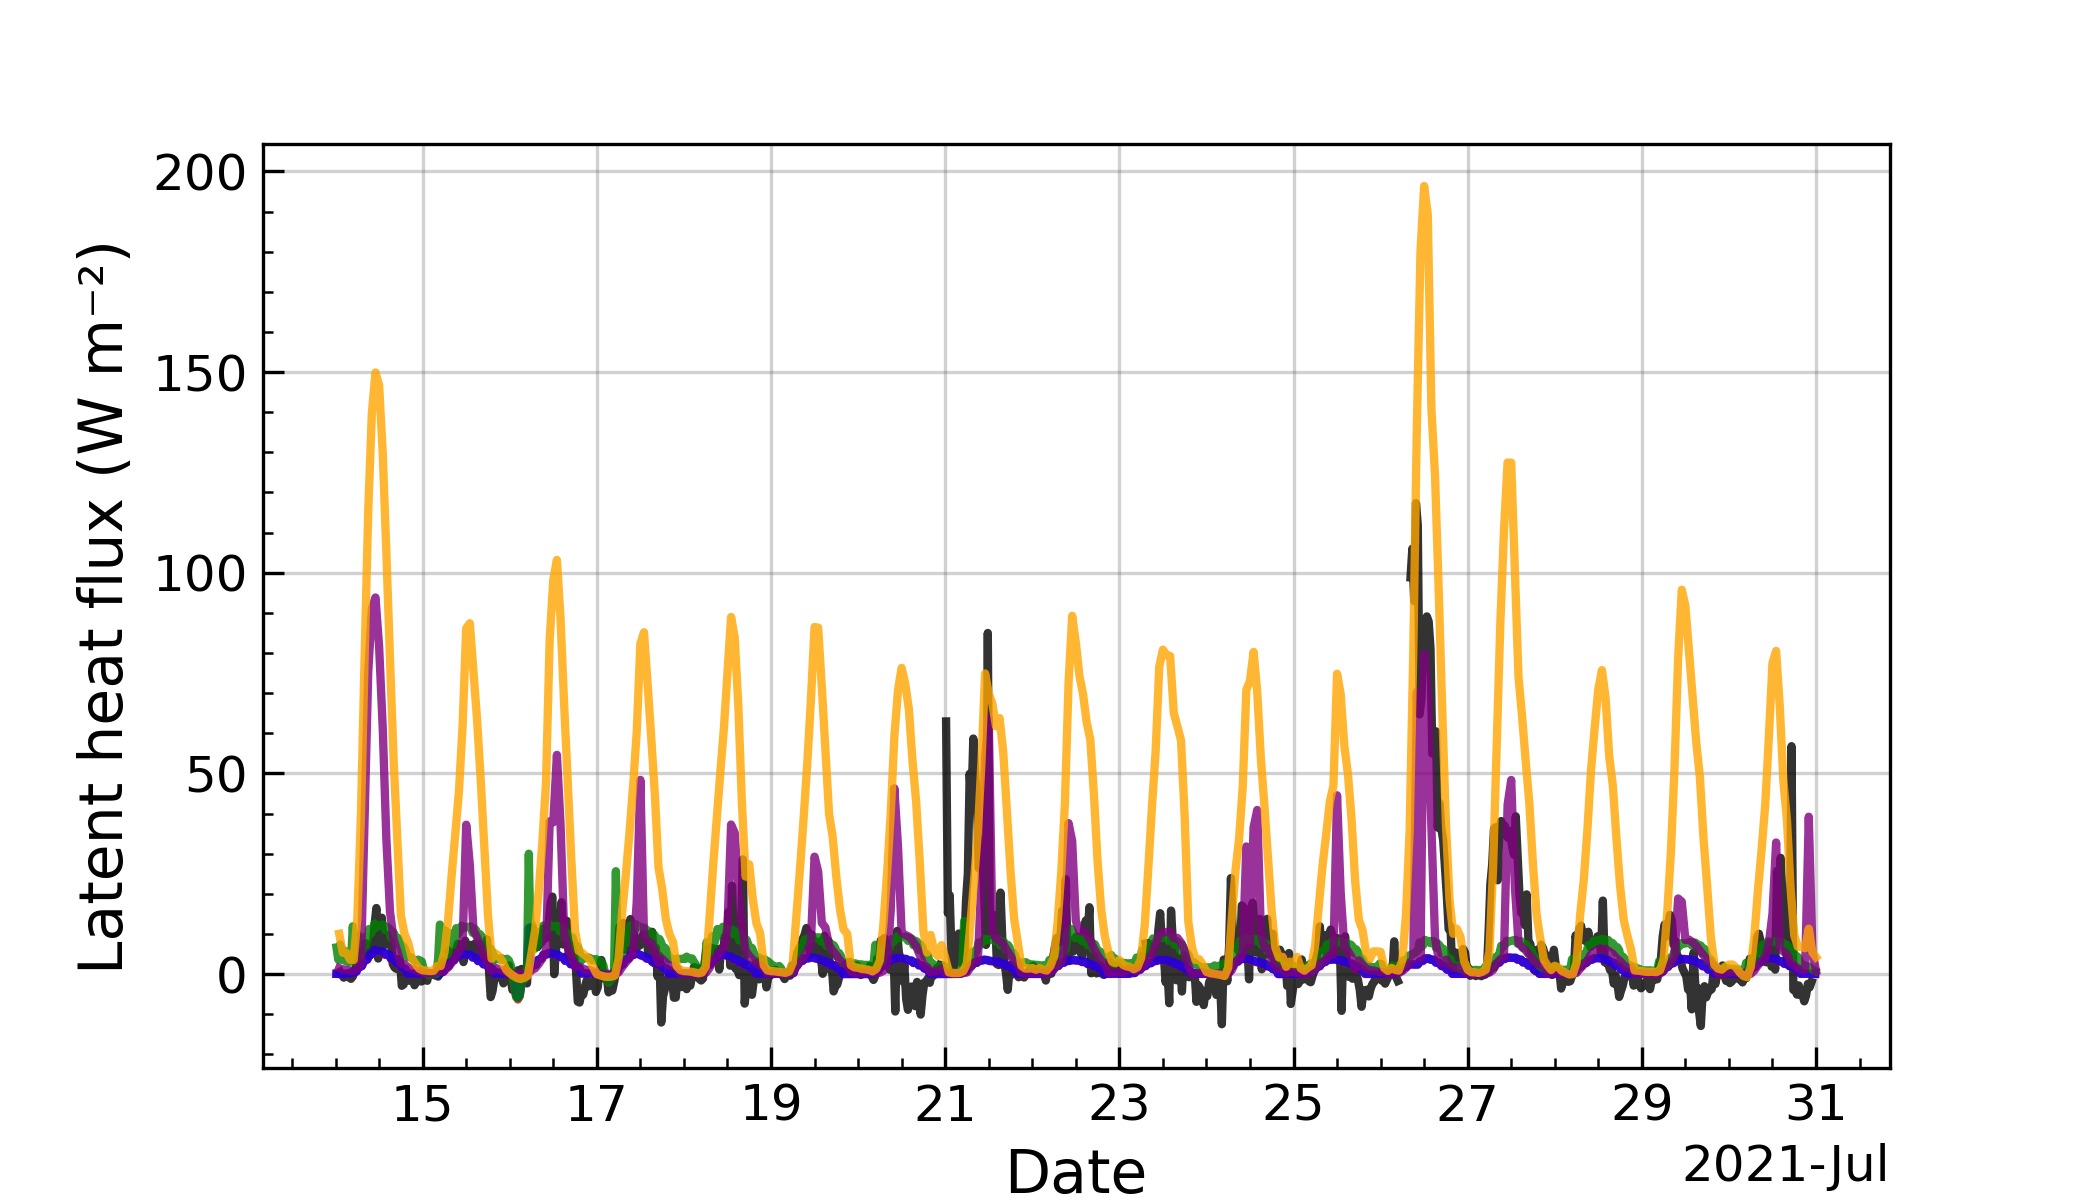
\includegraphics[width=\textwidth]{images/chap5/SOP_TS_DC/time_series_elsplans_flat.png}
        \end{subfigure} &
        \begin{subfigure}[t]{0.5\textwidth}
            \caption{}
            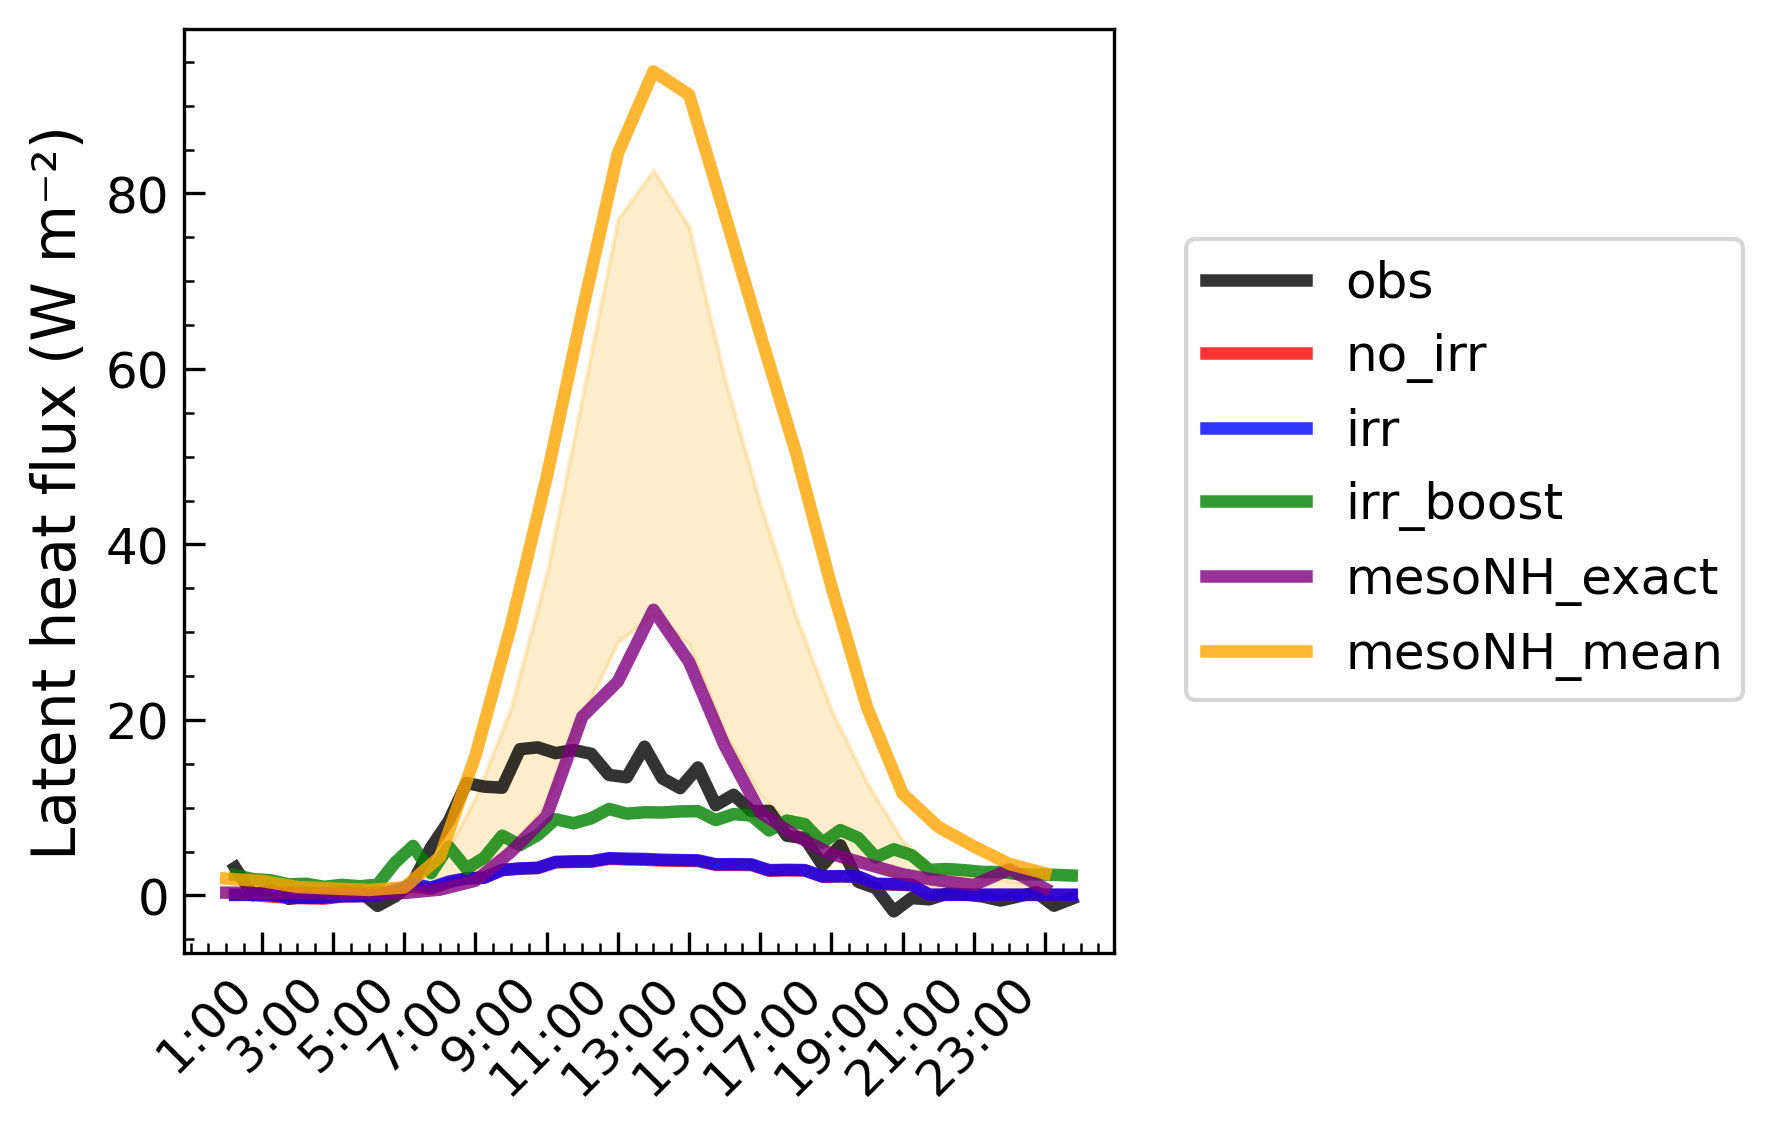
\includegraphics[width=\textwidth]{images/chap5/SOP_TS_DC/diurnal_cycle_elsplans_flat.png}
        \end{subfigure} \\
        \begin{subfigure}[t]{0.5\textwidth}
            \caption{}
            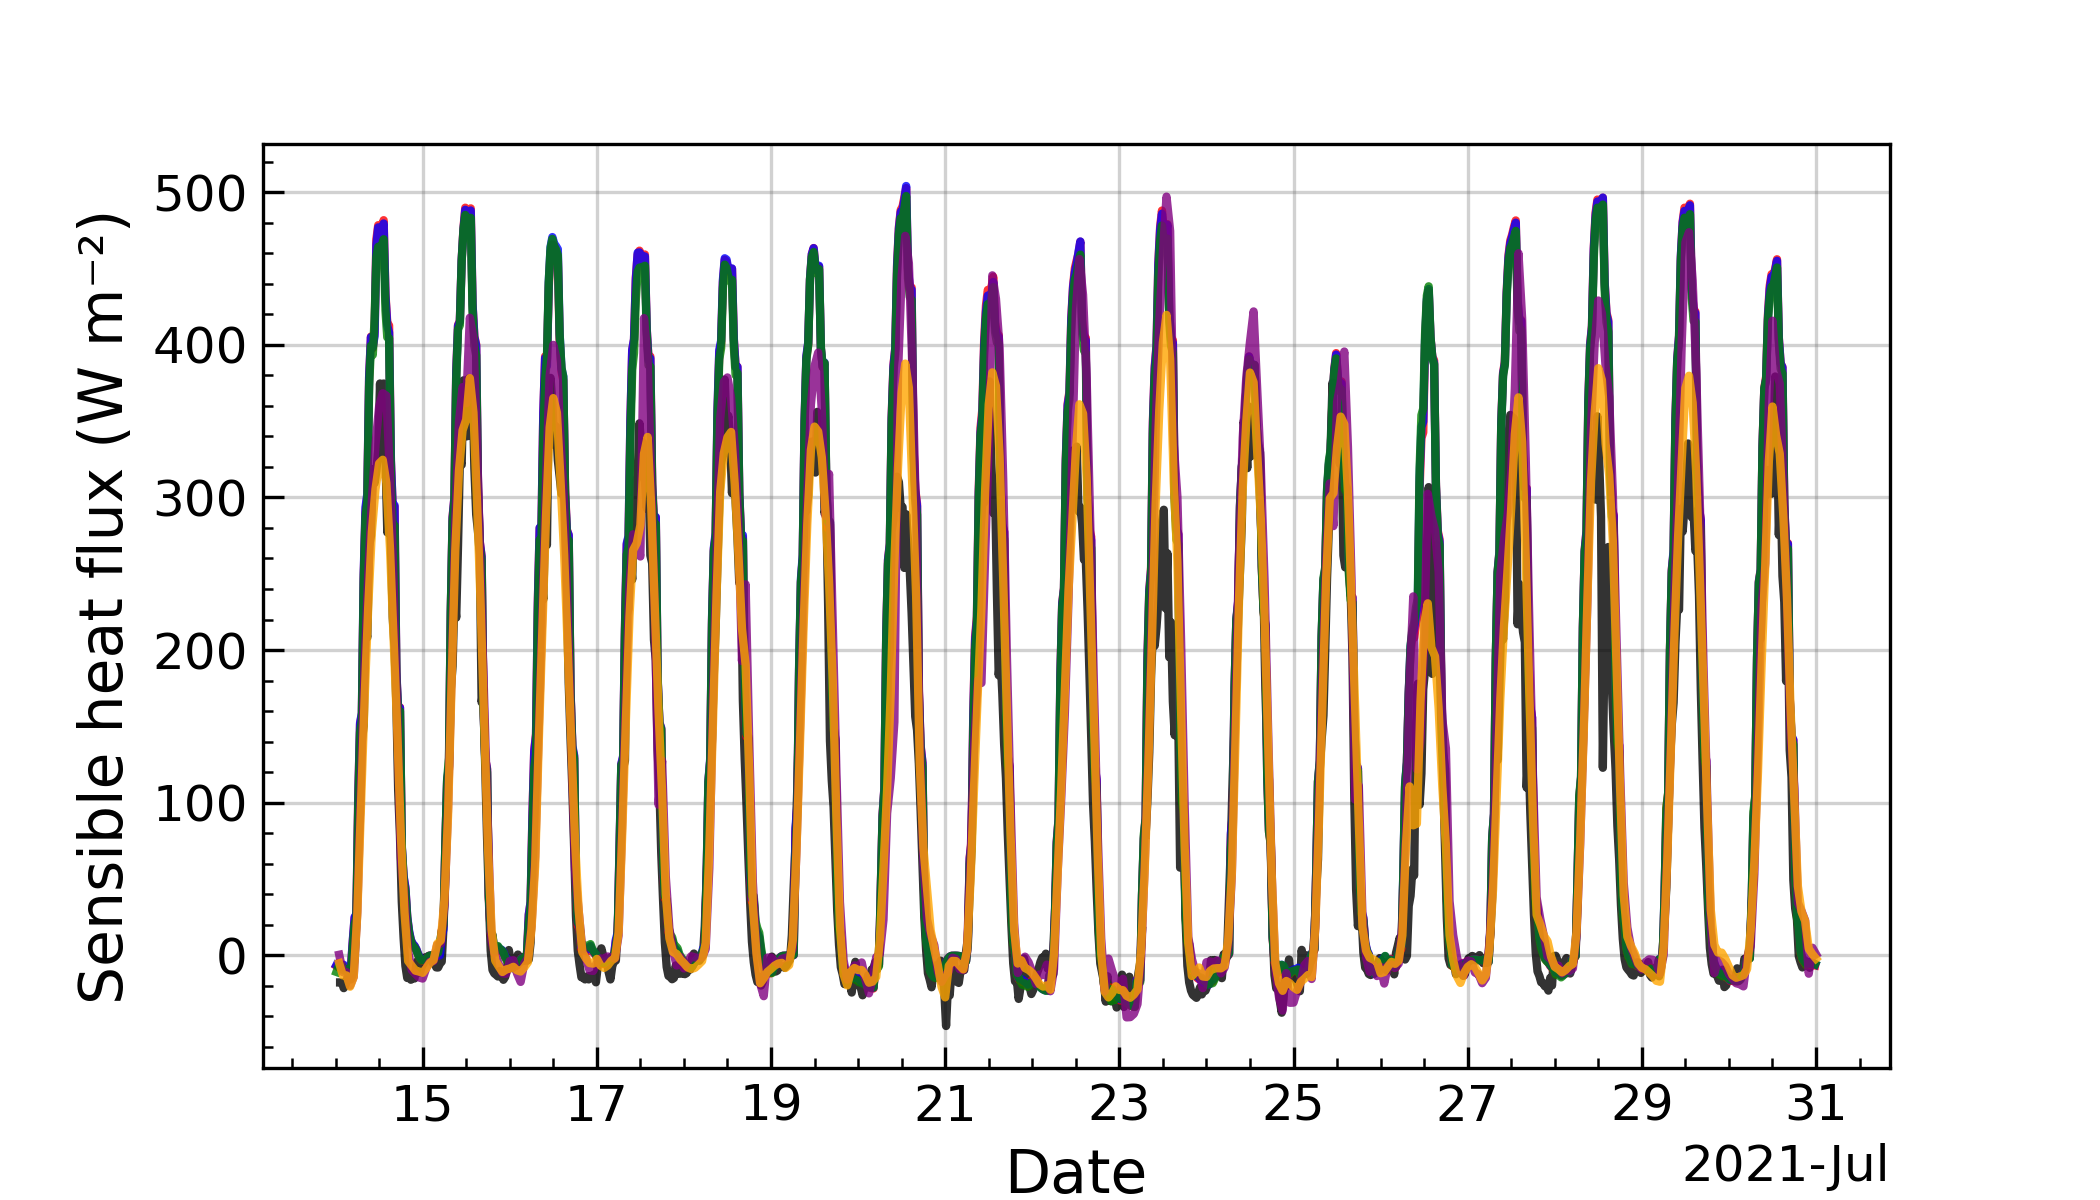
\includegraphics[width=\textwidth]{images/chap5/SOP_TS_DC/time_series_elsplans_sens.png}
        \end{subfigure} &
        \begin{subfigure}[t]{0.5\textwidth}
            \caption{}
            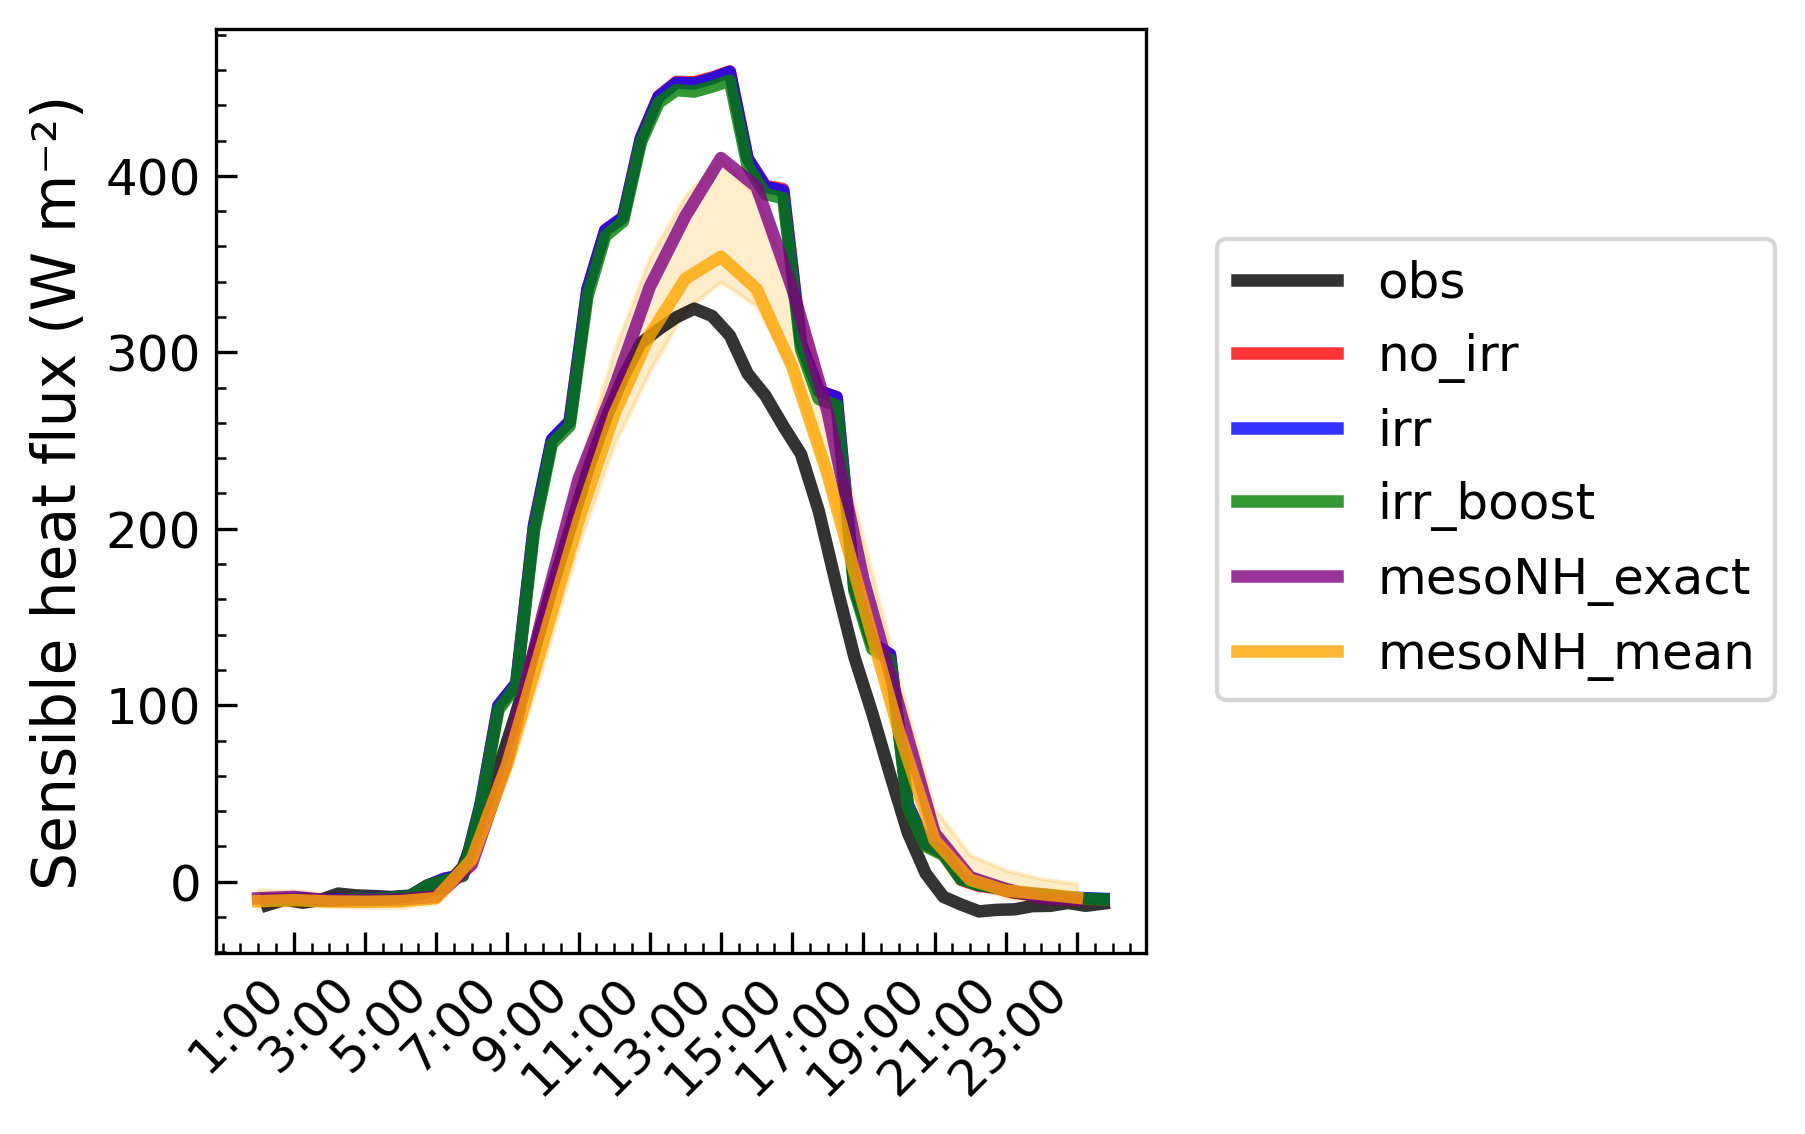
\includegraphics[width=\textwidth]{images/chap5/SOP_TS_DC/diurnal_cycle_elsplans_sens.png}
        \end{subfigure} \\
        \begin{subfigure}[t]{0.5\textwidth}
            \caption{}
            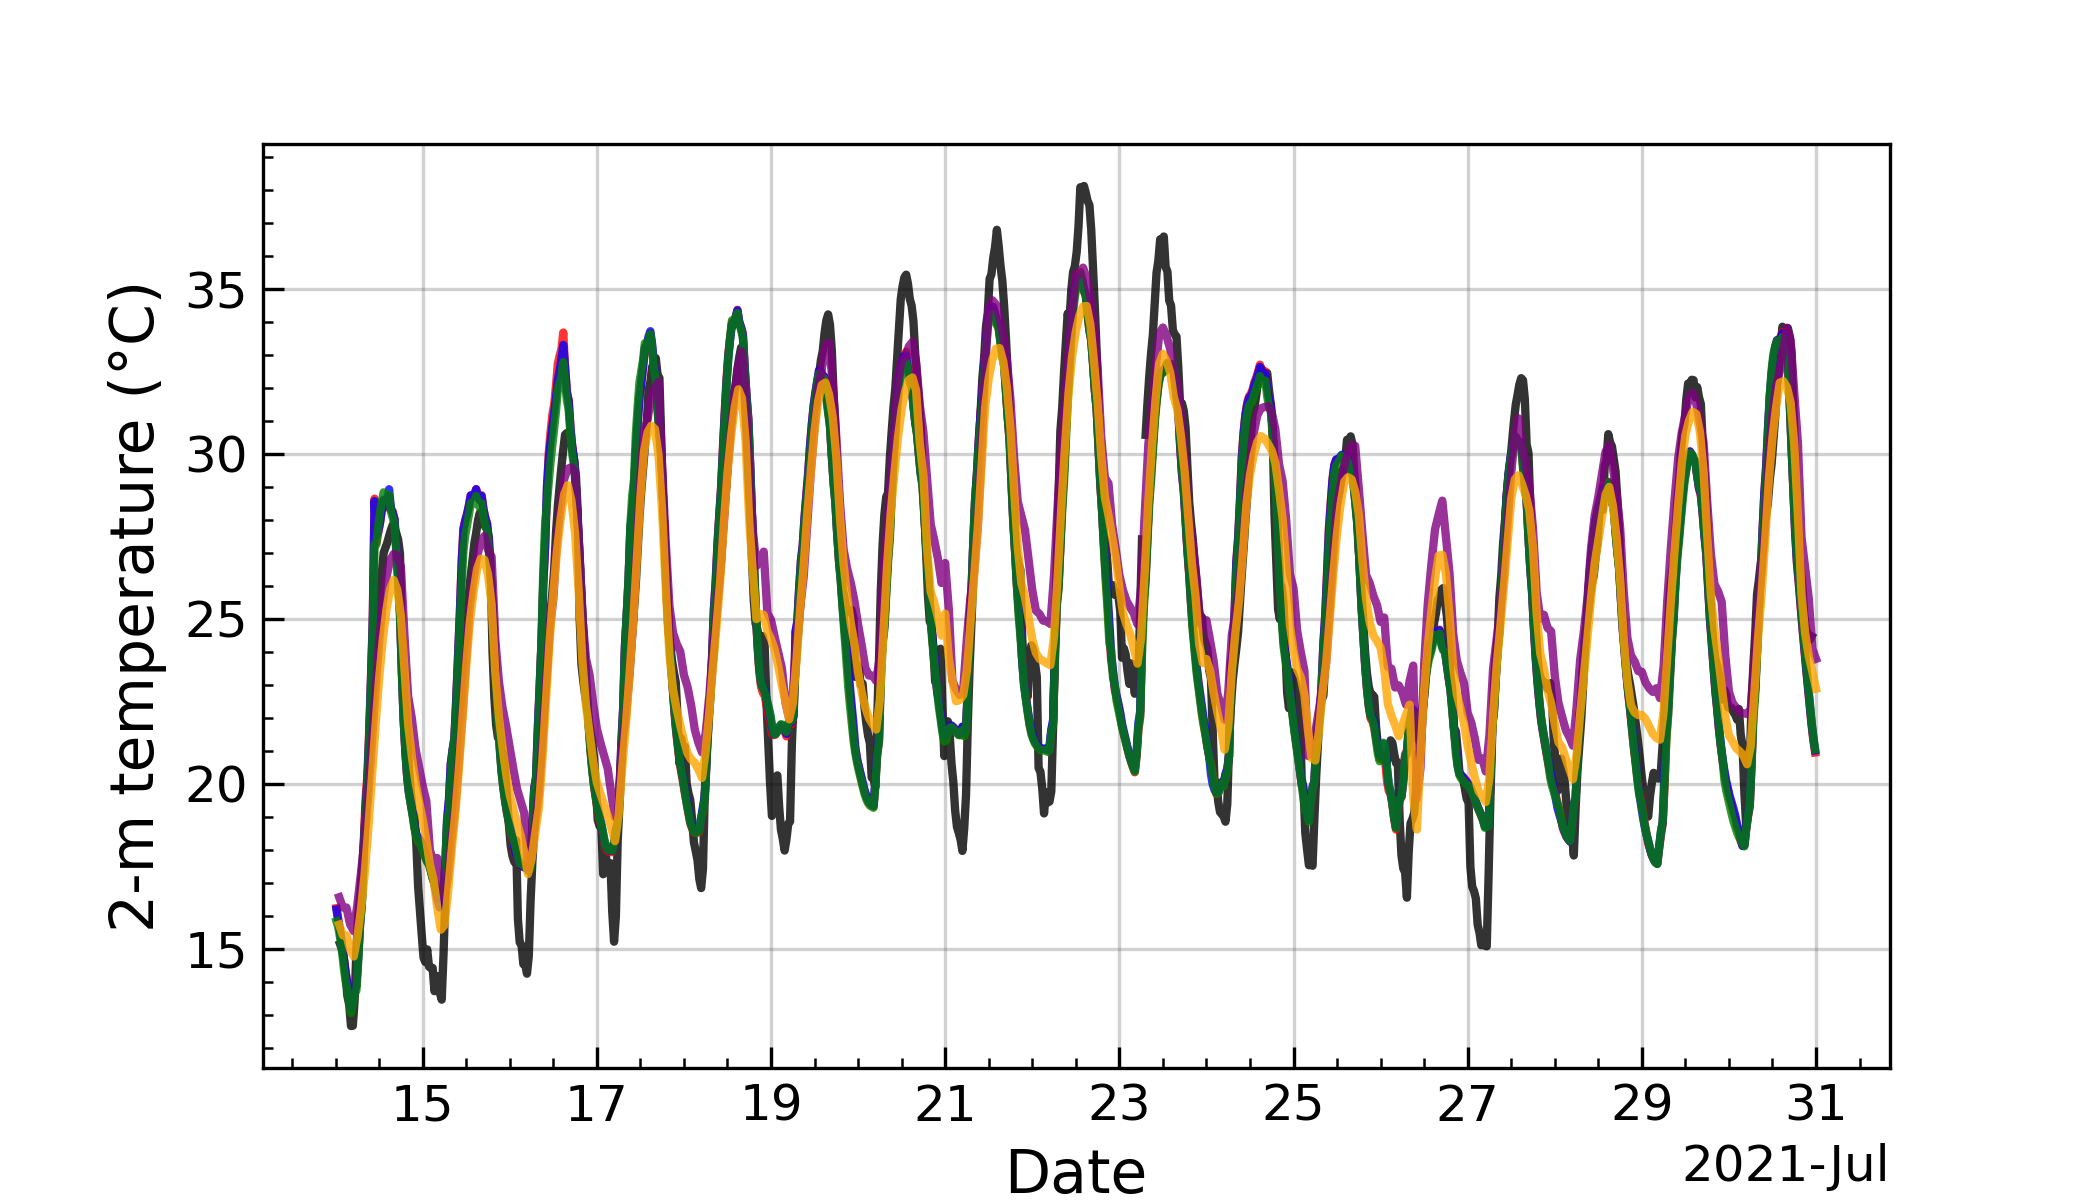
\includegraphics[width=\textwidth]{images/chap5/SOP_TS_DC/time_series_elsplans_t2m.png}
        \end{subfigure} &
        \begin{subfigure}[t]{0.5\textwidth}
            \caption{}
            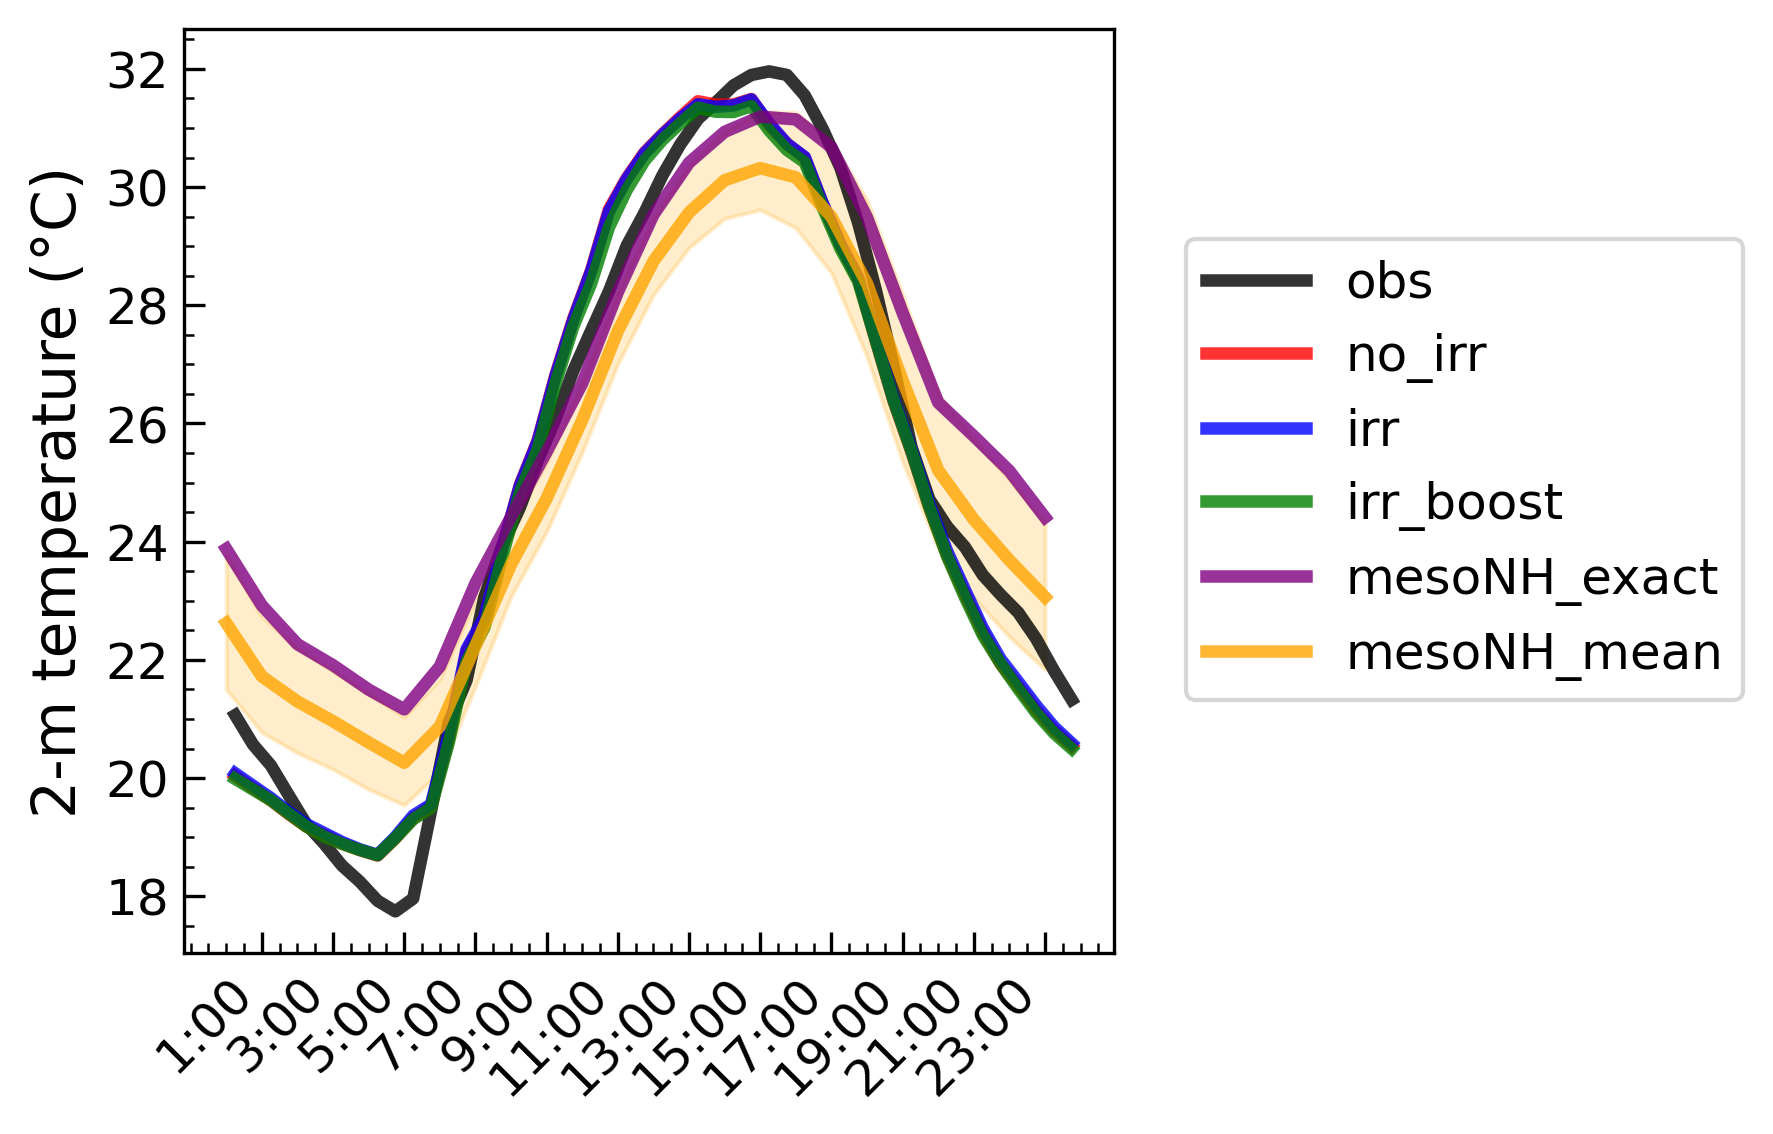
\includegraphics[width=\textwidth]{images/chap5/SOP_TS_DC/diurnal_cycle_elsplans_t2m.png}
        \end{subfigure} \\
        \begin{subfigure}[t]{0.5\textwidth}
            \caption{}
            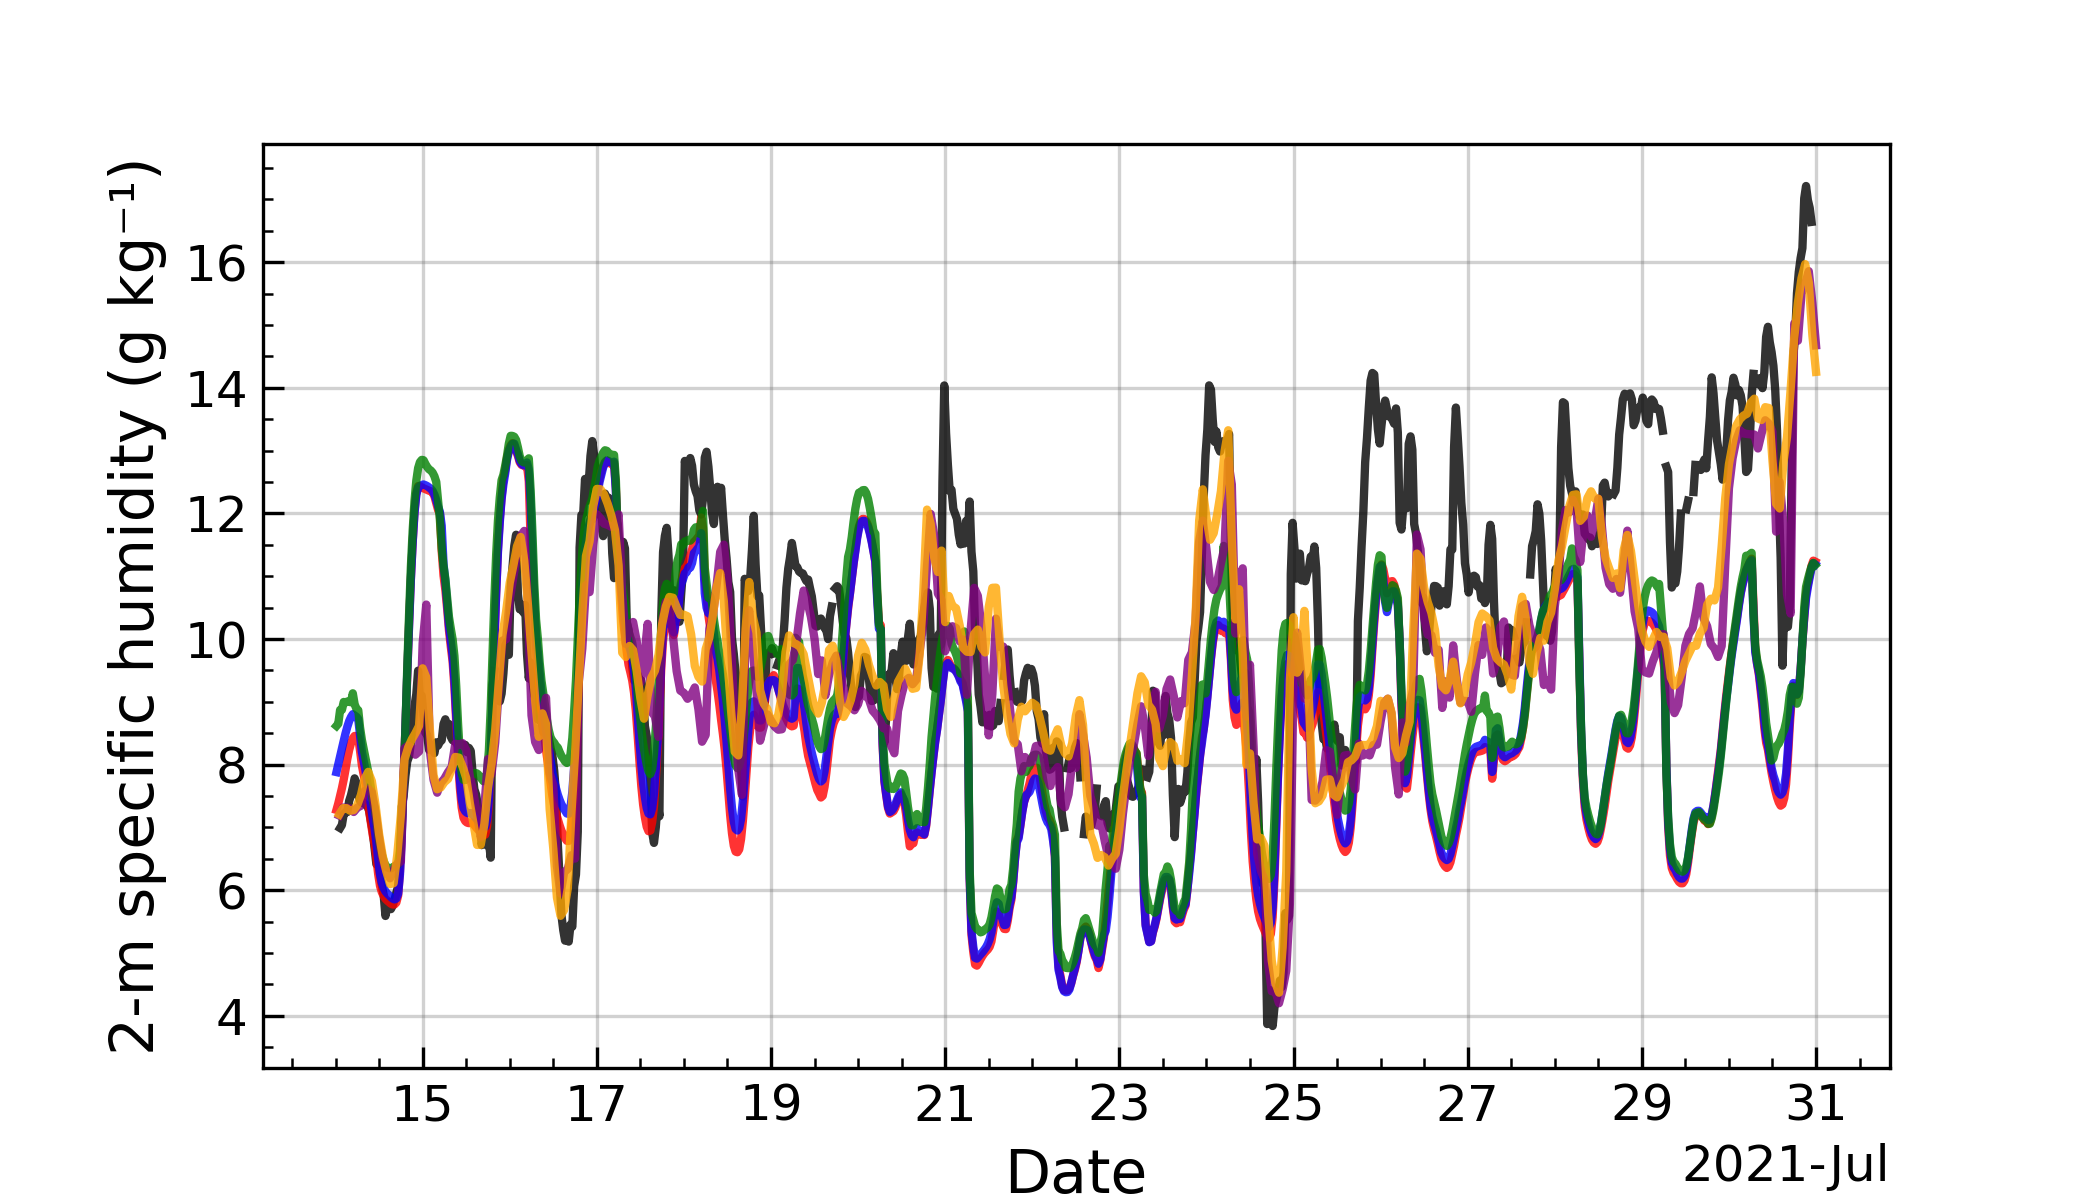
\includegraphics[width=\textwidth]{images/chap5/SOP_TS_DC/time_series_elsplans_q2m.png}
        \end{subfigure} &
        \begin{subfigure}[t]{0.5\textwidth}
            \caption{}
            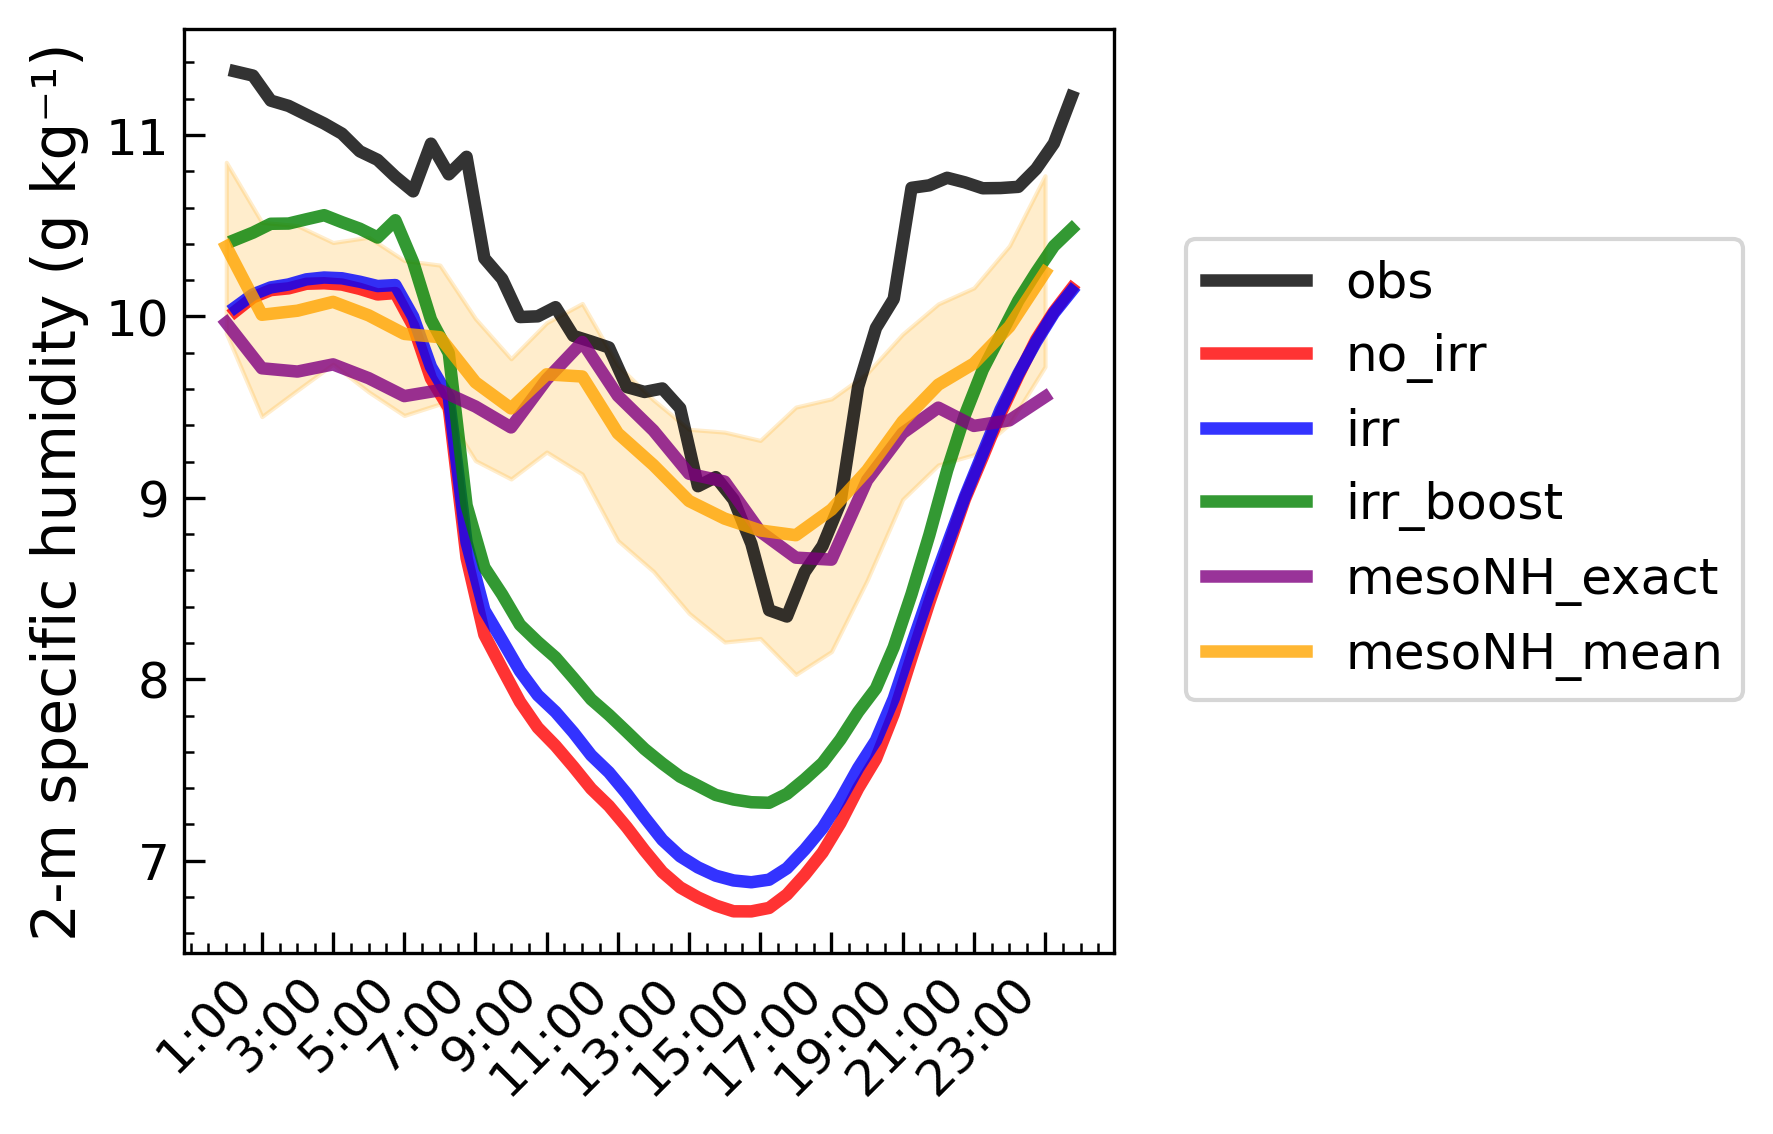
\includegraphics[width=\textwidth]{images/chap5/SOP_TS_DC/diurnal_cycle_elsplans_q2m.png}
        \end{subfigure}
    \end{tabular}
    \caption{Time series and mean diurnal cycle of surface turbulent fluxes at Els Plans (rainfed site), 14-30 July 2021. The envelope for \mesomean represents the 25th and 75th percentiles of the distribution.}
    \label{fig:elsplans_surfacevars}
\end{figure}

\hfill

%%CCL%%
The key takeaways from this comparison of near-surface variables over the SOP is that the irrigation parametrization can significantly improve the results at La Cendrosa, especially if irrigation demand is fully satisfied, as done in the \irrboost sensitivity experiment.
In particular, even if the observations cannot be matched perfectly, near-surface variables simulated by ICOLMDZOR are very close to the \mesomean values. Considering that the Meso-NH simulation is a relevant reference (ensured by the good performance of \mesoexact), it means that a good representation of grid-cell average values is achieved in the \irrboost simulation. 
In the second part of the SOP, a dry bias in ICOLMDZOR was identified, which could be improved be not entirely corrected by irrigation. Since this limitation is also visible at the rainfed site of Els Plans, and occurs simultaneously with a change in near-surface wind regime, it was hypothesized to be mainly the consequence of non-local effects, such as insufficient moisture advection over the LIAISE study area. The next section provides a study of the vertical structure of the ABL over two days, 15 July and 20 July, to investigate the differences between the first and second part of the SOP, and characterise the impact of irrigation and surface heterogeneities in these two different contexts.
\clearpage %todo:keep ?

\section{Vertical structure of the atmosphere}
\label{sec:iop}

Out of the seven IOP days over which radiosoundings were conducted on both sites, two were selected (15 July and 20th) to further investigate the atmospheric behaviour of the ICOLMDZOR LAM and the impact of irrigation on the vertical structure of the ABL.

\subsection{Surface conditions on selected IOP days}
%todo:reorganize, describe obs for all vars and then comment on model performance ?
%mesoexact is very very good on most vars, making it an interesting reference

15 July was selected as a representative IOP day for the beginning of the SOP, showing similarities with observed profiles on the 16th and 17th. As the SOP progressed, 2-meter temperature increased and the wind regime became much more changeable, with more influence from the sea breeze circulation.
The three following IOP days (20th, 21st, 22nd) therefore presented different conditions, and this is why 20 July was also selected to analyse the impacts of irrigation on the ABL under different conditions.

The time series at La Cendrosa over both days (Fig. \ref{fig:iop_days_TS_surfvars}) clearly show that 20 July was a warmer and moister day than 15 July, with important variations in wind speed and direction.
%LMDZ biases in t2m, q2m
At the surface, ICOLMDZOR presents a warm bias on 15 July of varying amplitude depending on irrigation intensity, but on 20 July, this bias is of smaller amplitude, and even suppressed in the daytime in the \irrboost simulation.
As previously noticed in general over the SOP, 2-m specific humidity is overestimated by ICOLMDZOR at night, but decreases during the day. In \irrboost, it remains slightly above observed and Meso-NH values during the day on 15 July, but on 20 July it is underestimated.
%link to flat?
This may partly be explained by the differences in latent heat flux between the two days. As mentionned in Section \ref{sec:sop}, at the beginning of the SOP, crops had recently been cut and plant transpiration was not at its usual level.
Since the models do not account for this information, the latent heat flux is overestimated by Meso-NH (both \mesoexact and \mesomean are above the observations) and ICOLMDZOR in the \irrboost simulation, whereas the sensible heat flux is underestimated (Fig. \ref{fig:iop_days_TS_energy}e, g). 
On 20 July, the observed latent heat flux is higher and the sensible heat flux lower, even presenting negative values in the afternoon.
For both turbulent fluxes, as noticed in Section \ref{sec:sop}, the \irrboost simulation matches really well the \mesomean aggregated value throughout the day, confirming that ICOLDMZOR properly represents the grid-cell averaged fluxes.
However although \mesomean has the same surface fluxes as \irrboost and very close values of 2-meter tempereature, it does not present the same biases in 2-meter specific humidity. As analysed in Section \ref{sec:sop}, near-surface humidity seems to be influenced by non-local processes on 20 July and the following days, hinting to an incorrect moisture advection in the ICOLMDZOR simulations. 
Here, the observed 10-m wind in the morning is very low and mainly comes from the North-Northwest (NNW), which is captured by Meso-NH, whereas ICOLMDZOR simulates an increasingly stronger wind from the East-Southeast (ESE). 
%option:remove mention of sea breeze in the afternoon ? Focus on general conditions and 12UTC ?
In the afternoon, observations show a rapid change in wind direction to a southeasterly wind, associated with an increase in wind speed from less than 1 m \persec to more than 5 m \persec. That sudden variation is very likely associated with a sea breeze phenomenon bringing moist air from the Mediterranean sea. %option:note that regional topography is complexe and sea breeze sometimes interferes with Catalan PreCoastal Range... Lunel et al 2024

%Fig : surface variables Cendrosa
\begin{figure}[hbtp]
    \centering
    \begin{tabular}{cc}
        %t2m, q2m
        \begin{subfigure}[t]{0.5\textwidth}
            \caption{}
            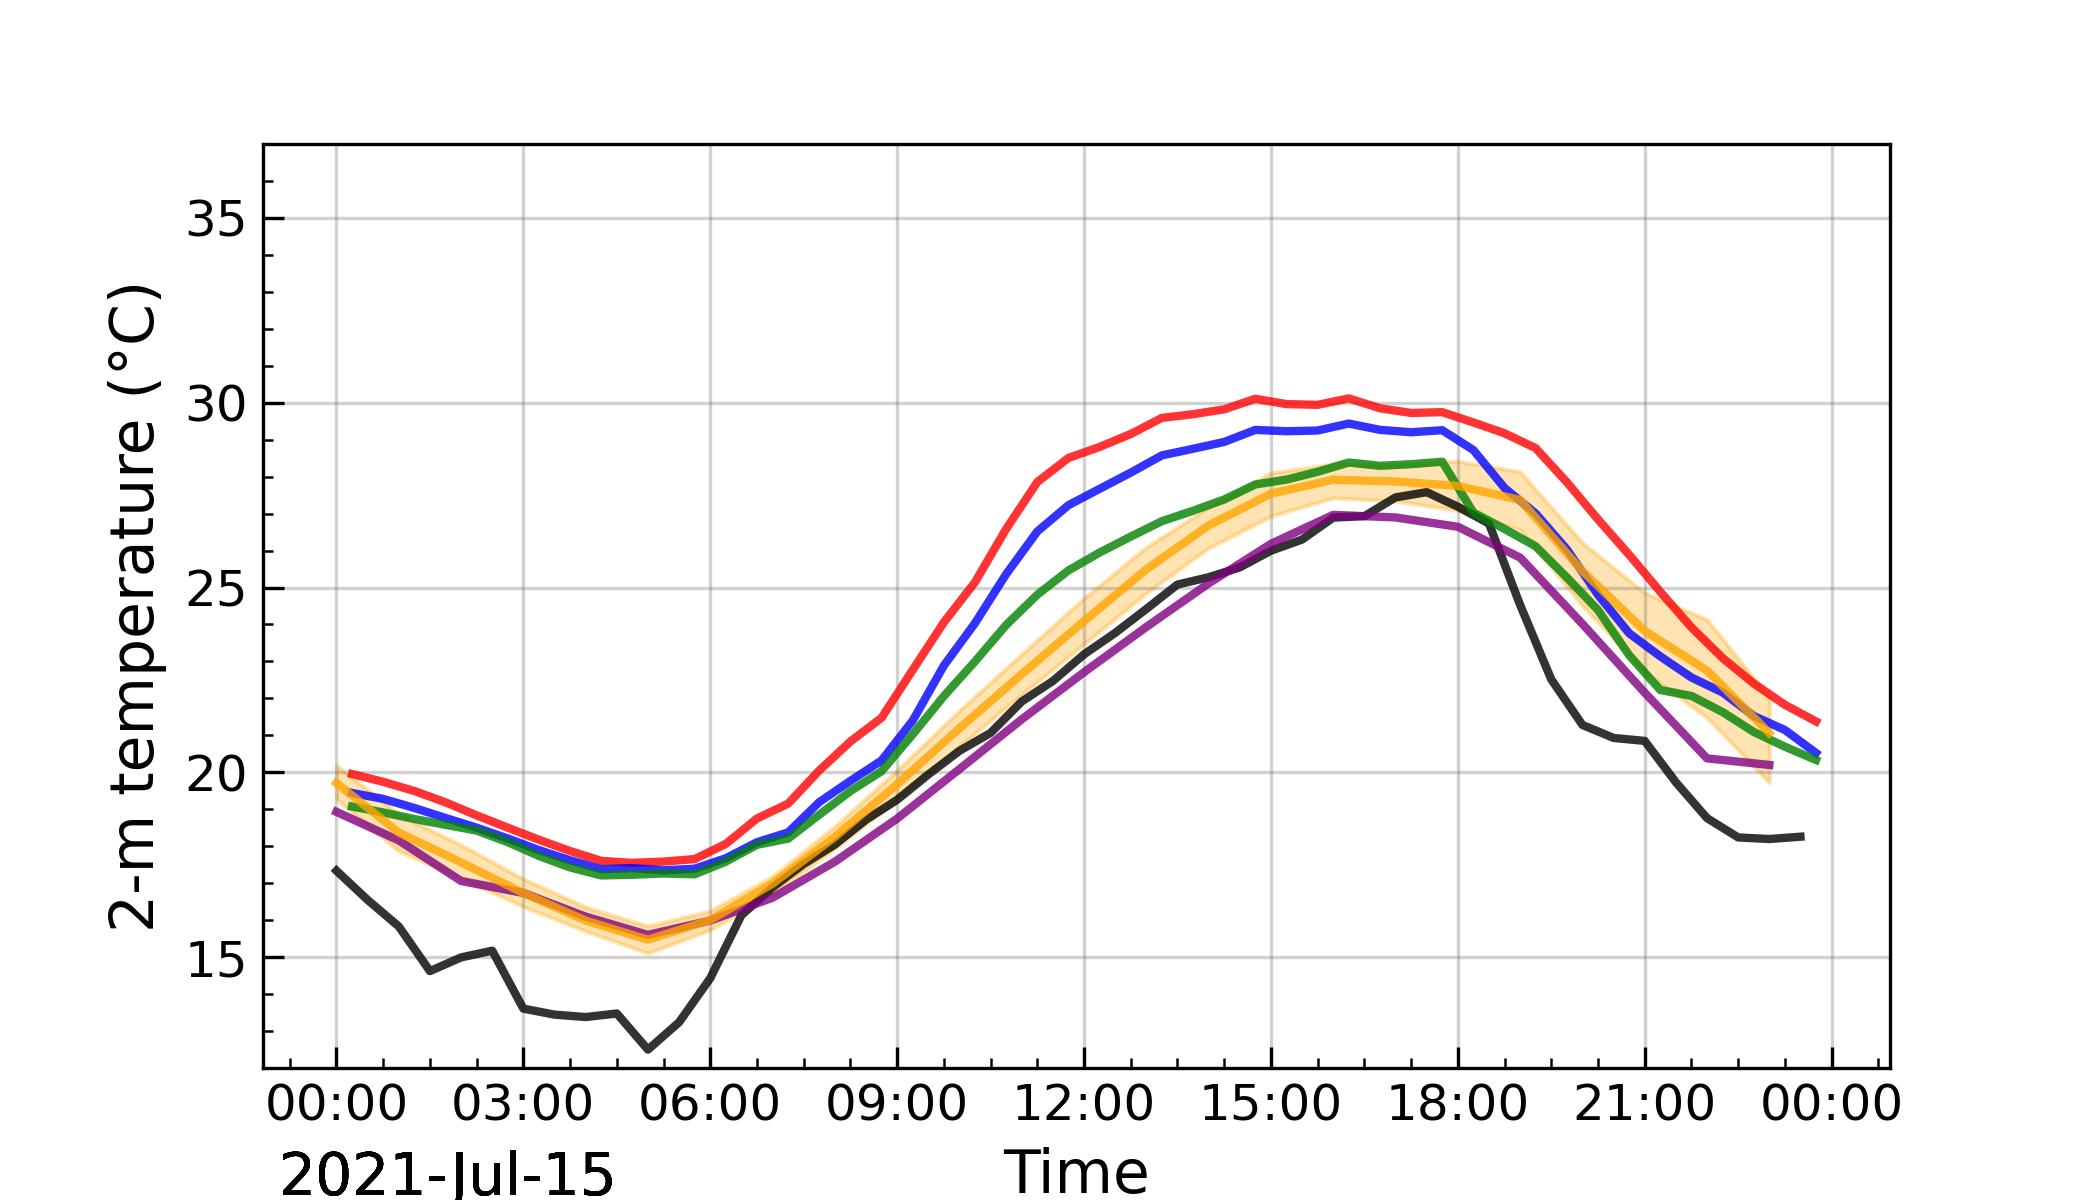
\includegraphics[width=\textwidth]{images/chap5/IOP_TS/TS_2021-07-15_cendrosa_t2m.png}
        \end{subfigure} &
        \begin{subfigure}[t]{0.5\textwidth}
            \caption{}
            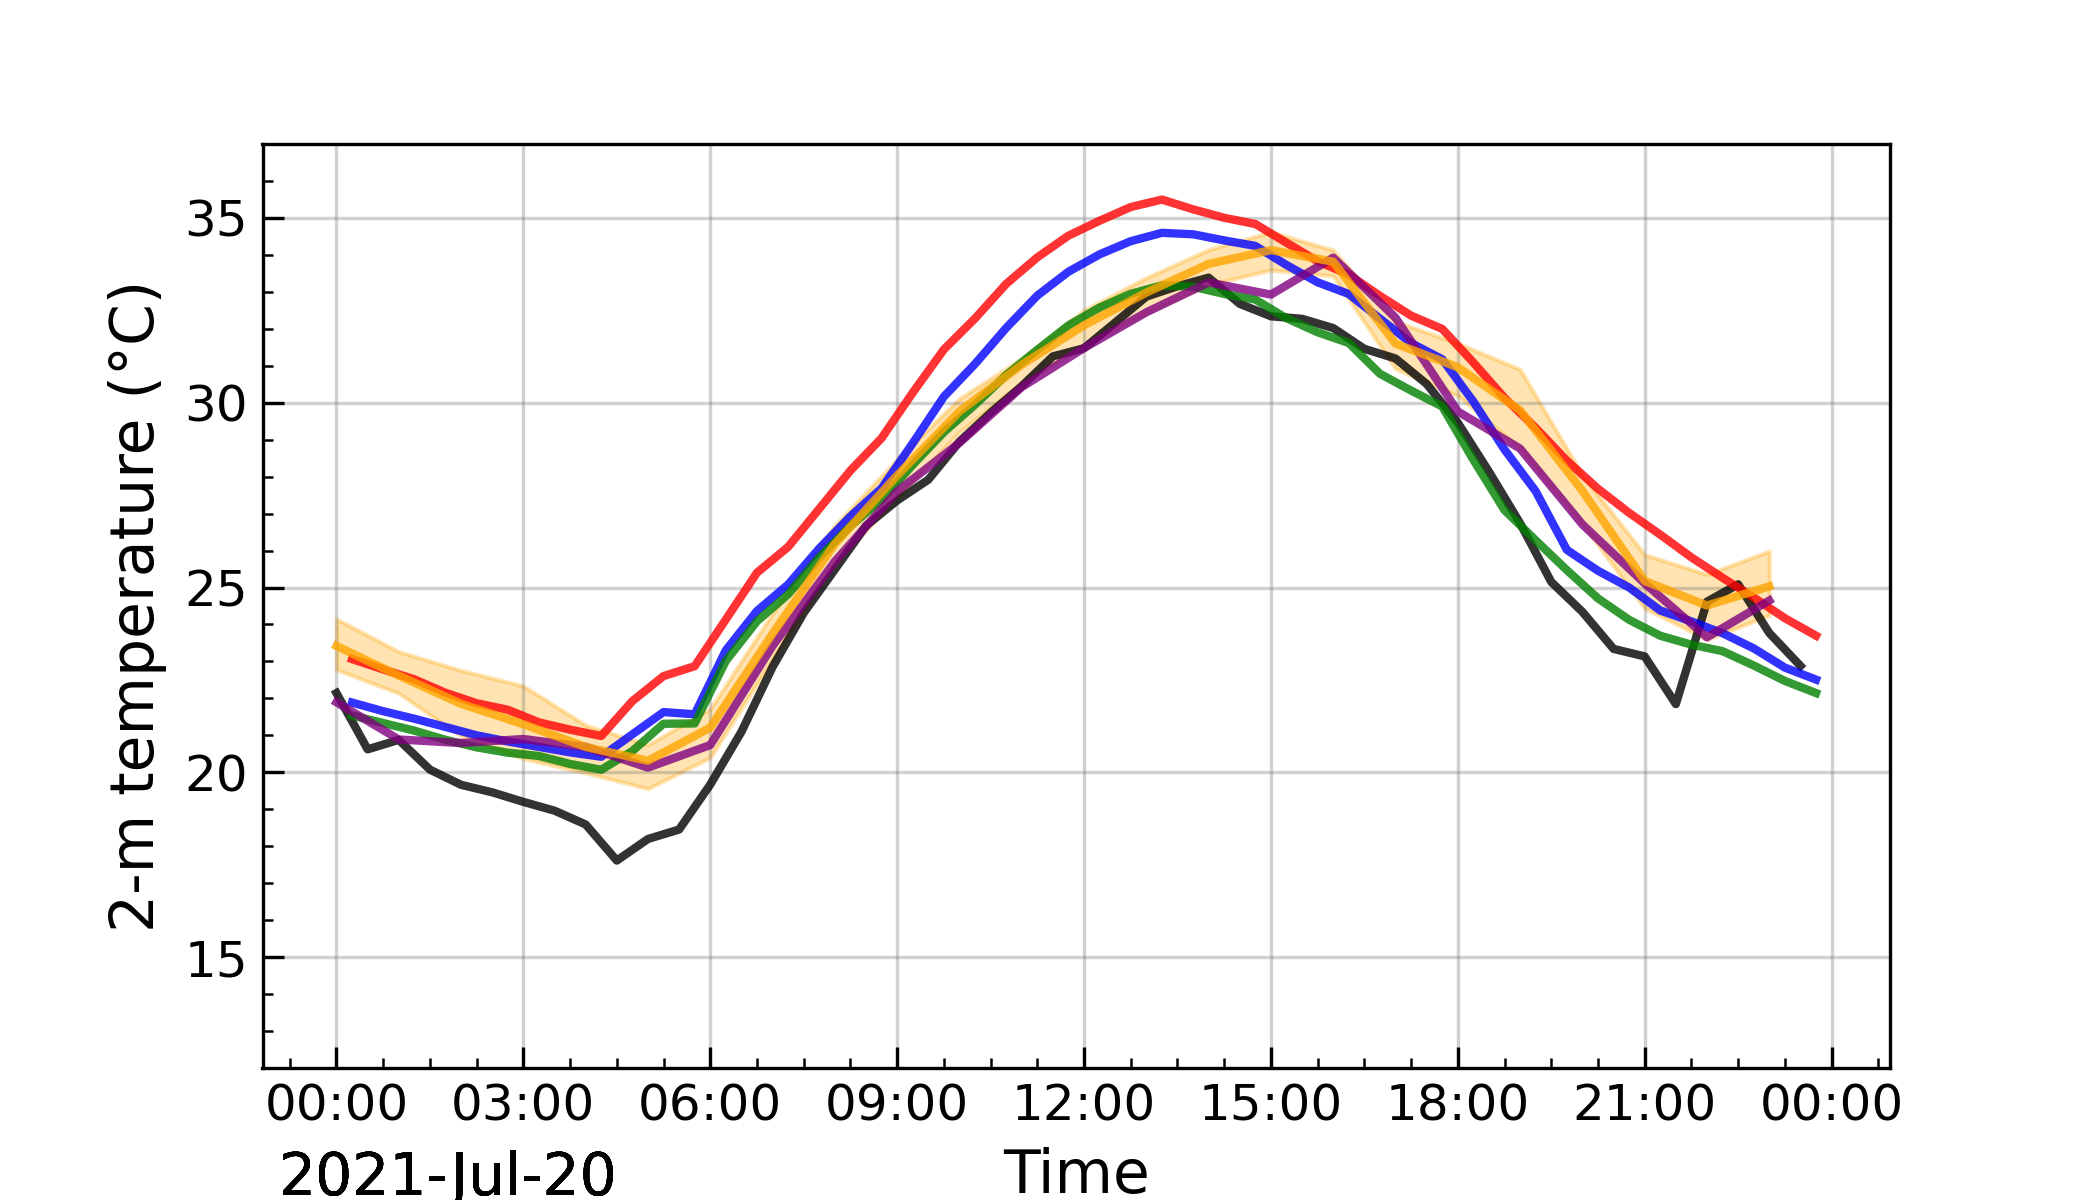
\includegraphics[width=\textwidth]{images/chap5/IOP_TS/TS_2021-07-20_cendrosa_t2m.png}
        \end{subfigure} \\
        \begin{subfigure}[t]{0.5\textwidth}
            \caption{}
            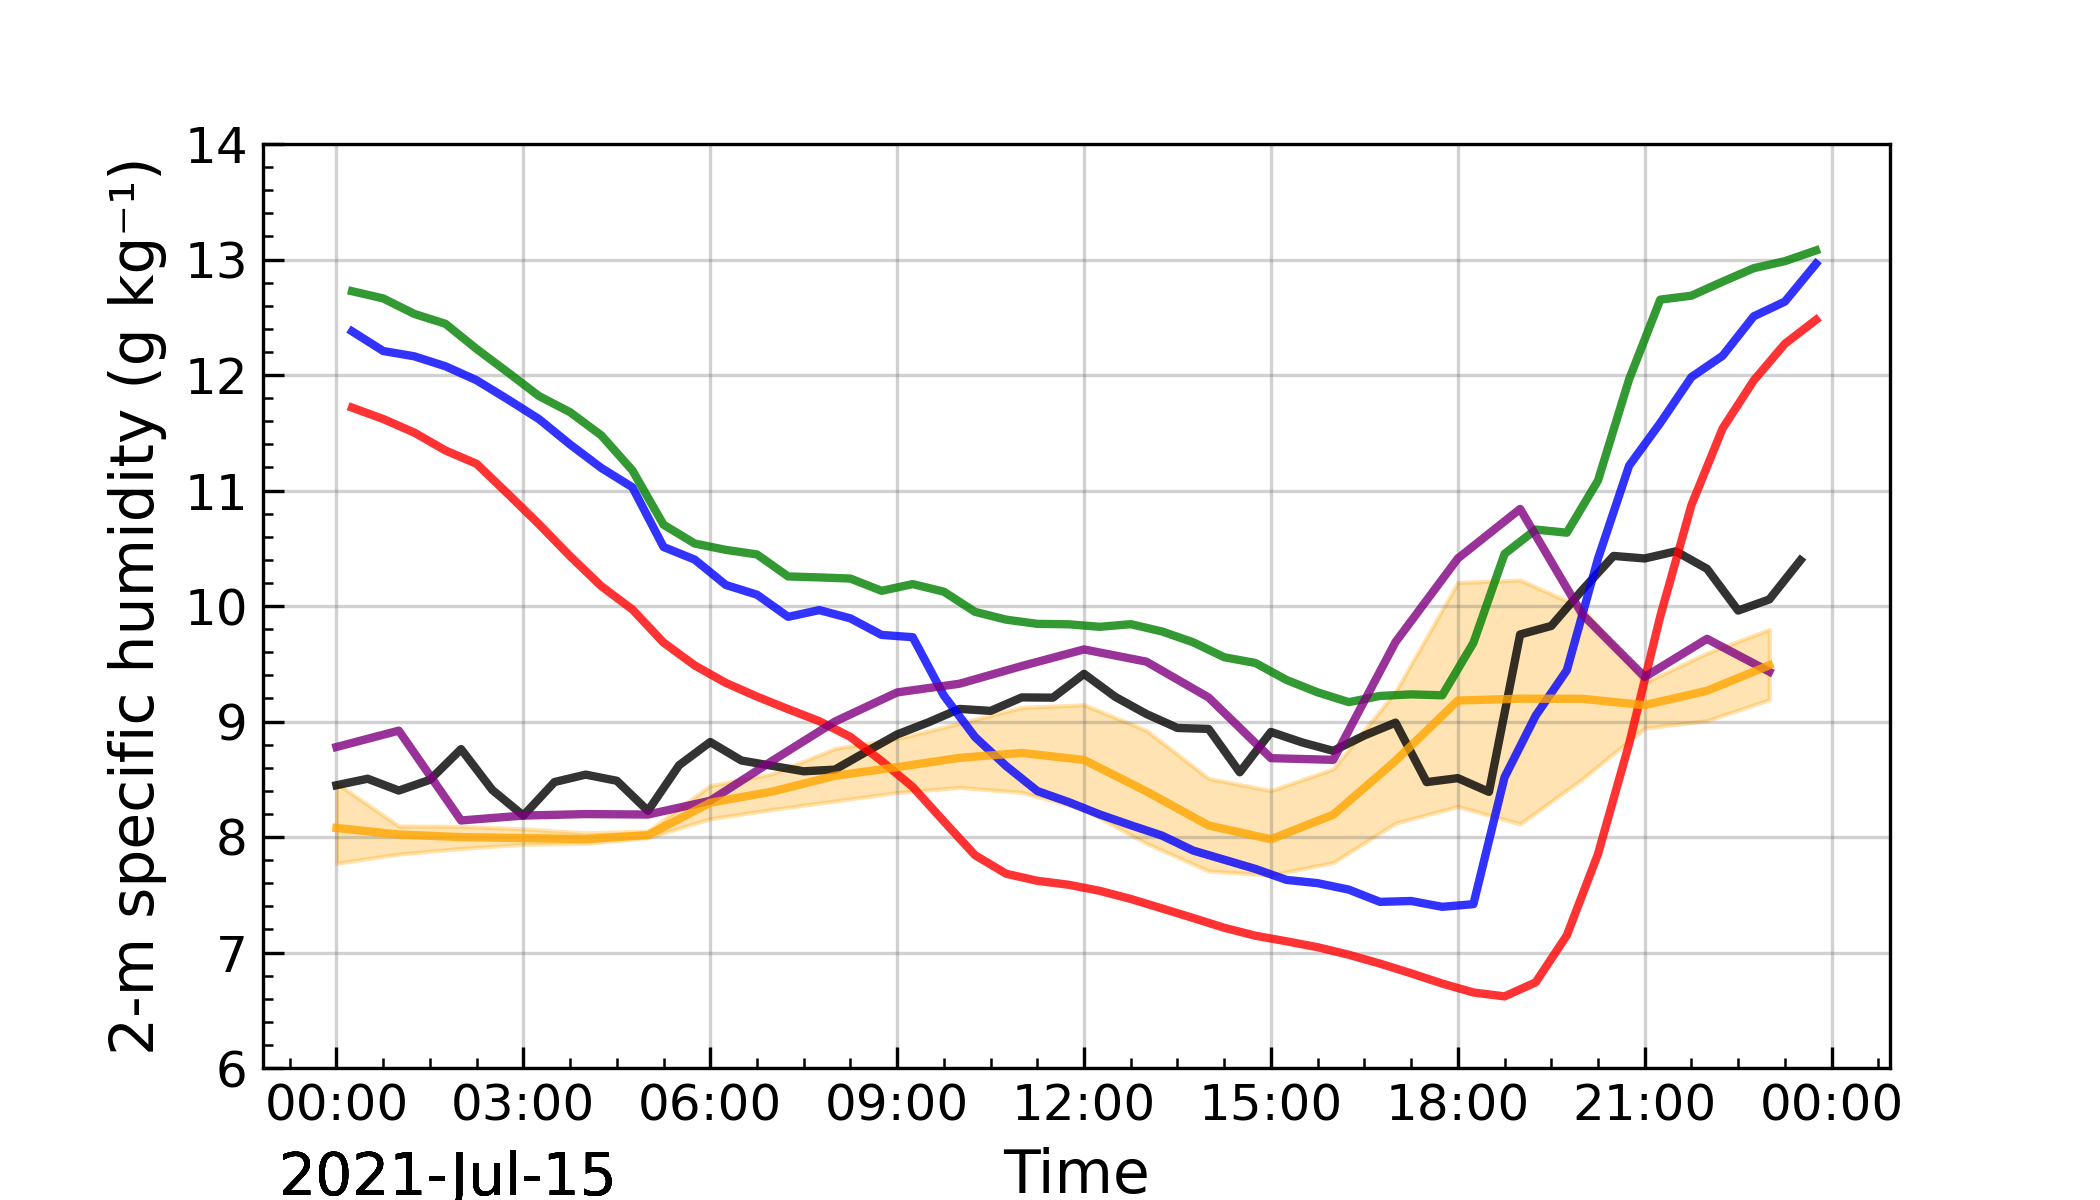
\includegraphics[width=\textwidth]{images/chap5/IOP_TS/TS_2021-07-15_cendrosa_q2m.png}
        \end{subfigure} &
        \begin{subfigure}[t]{0.5\textwidth}
            \caption{}
            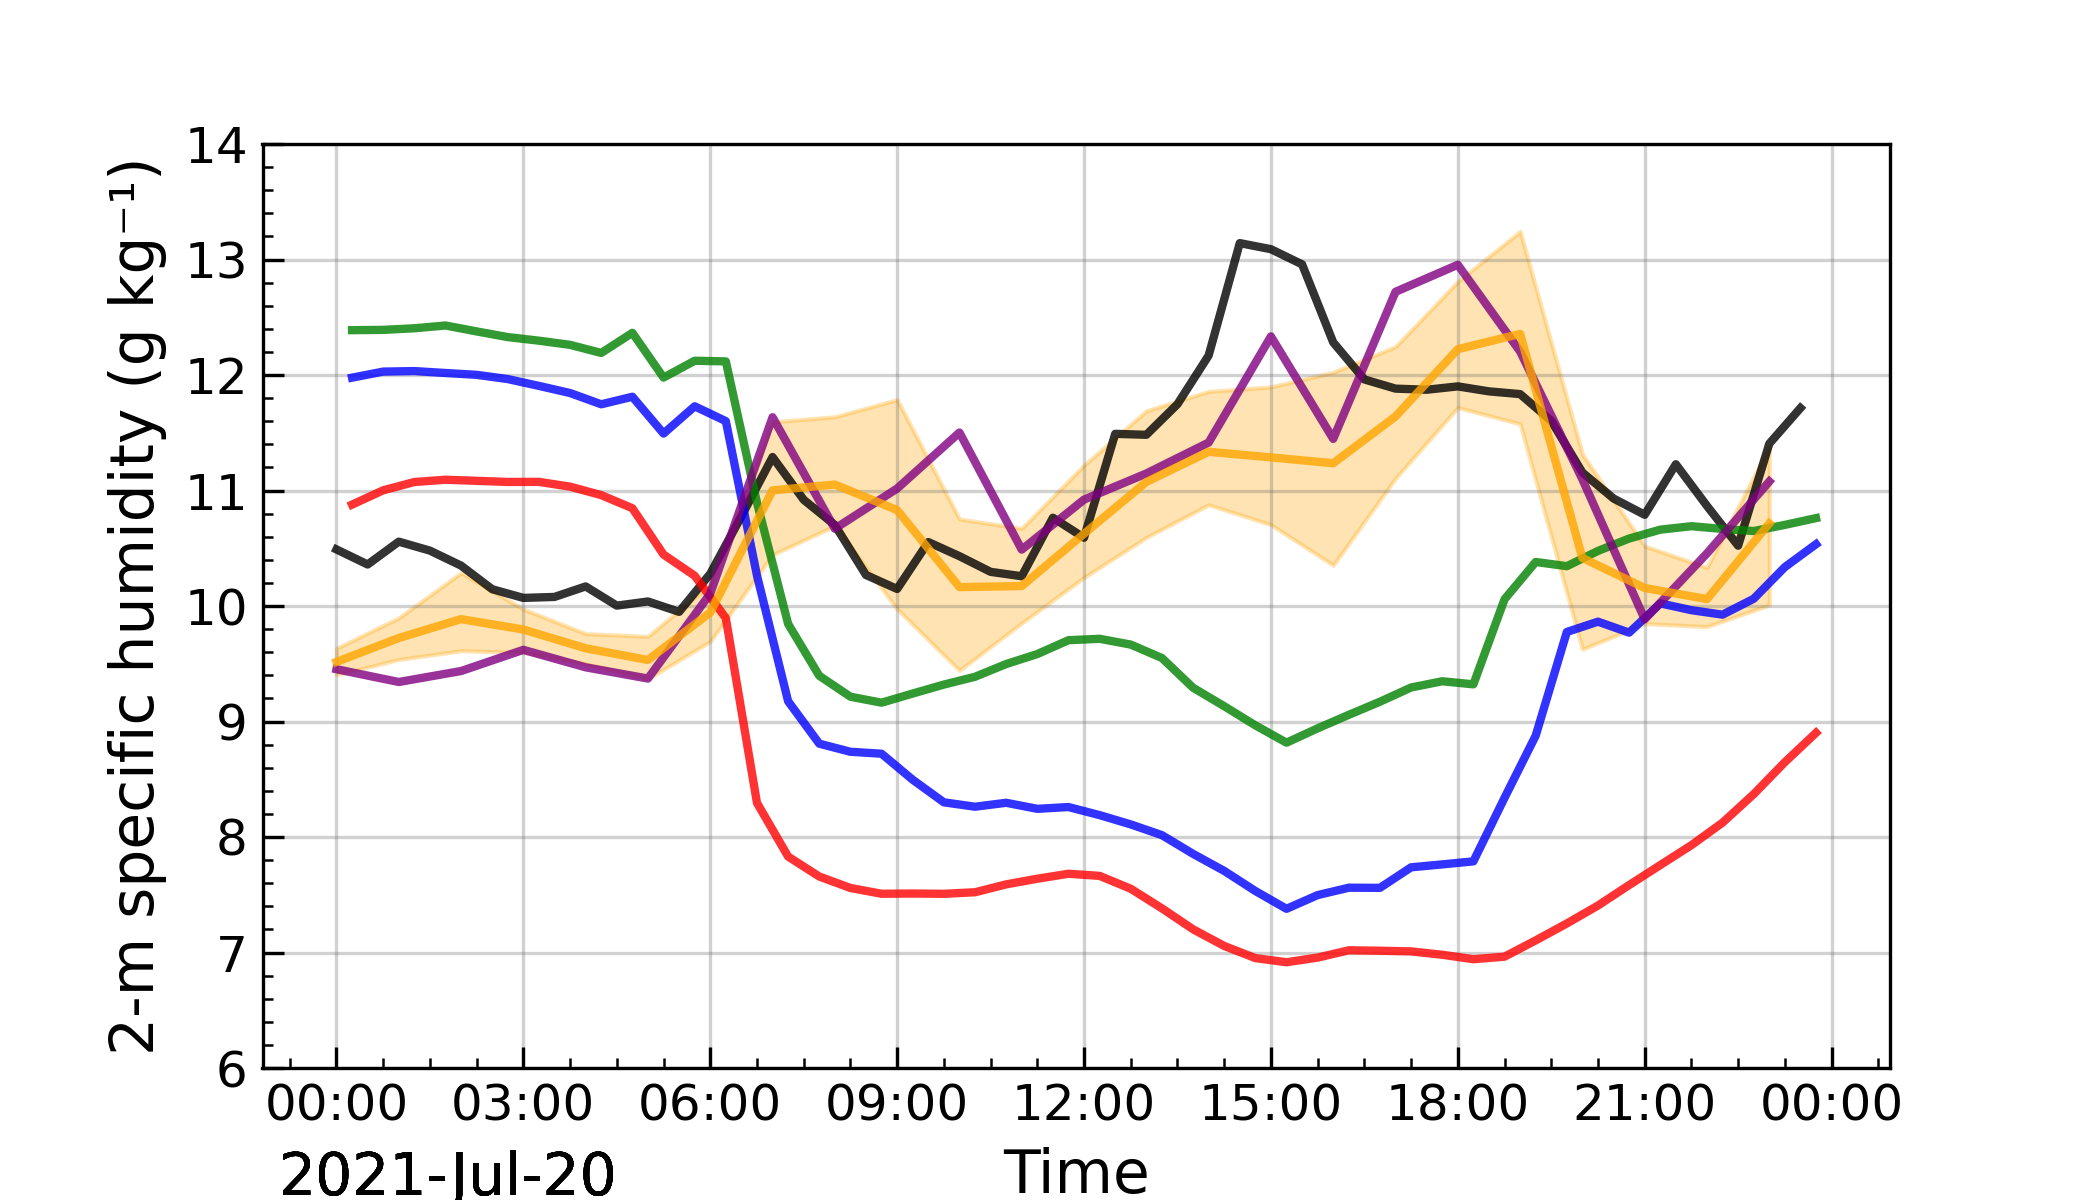
\includegraphics[width=\textwidth]{images/chap5/IOP_TS/TS_2021-07-20_cendrosa_q2m.png}
        \end{subfigure} \\

        %turb fluxes
        \begin{subfigure}[t]{0.5\textwidth}
            \caption{}
            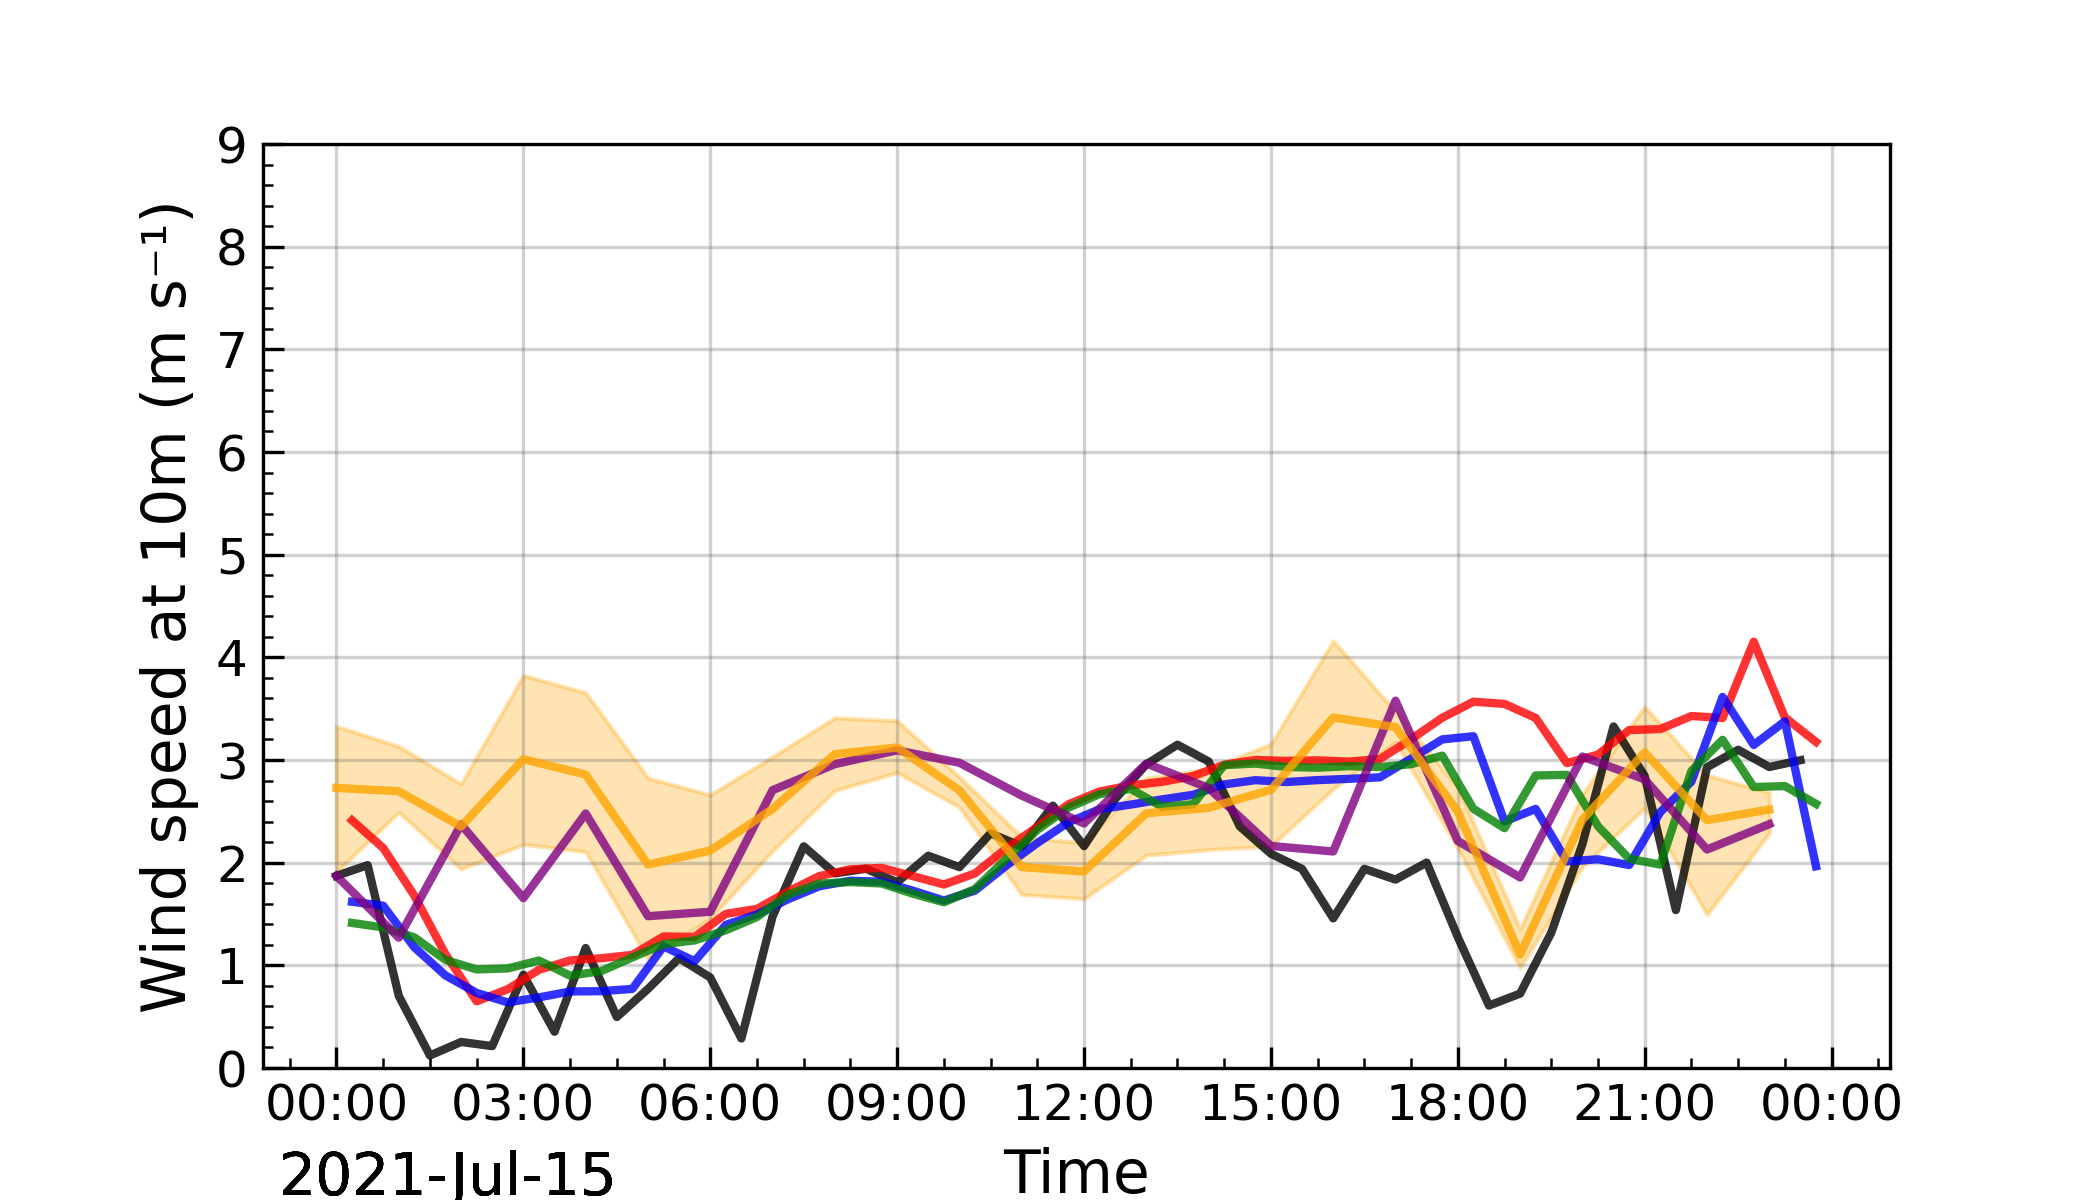
\includegraphics[width=\textwidth]{images/chap5/IOP_TS/TS_2021-07-15_cendrosa_wind_speed_10m.png}
        \end{subfigure} &
        \begin{subfigure}[t]{0.5\textwidth}
            \caption{}
            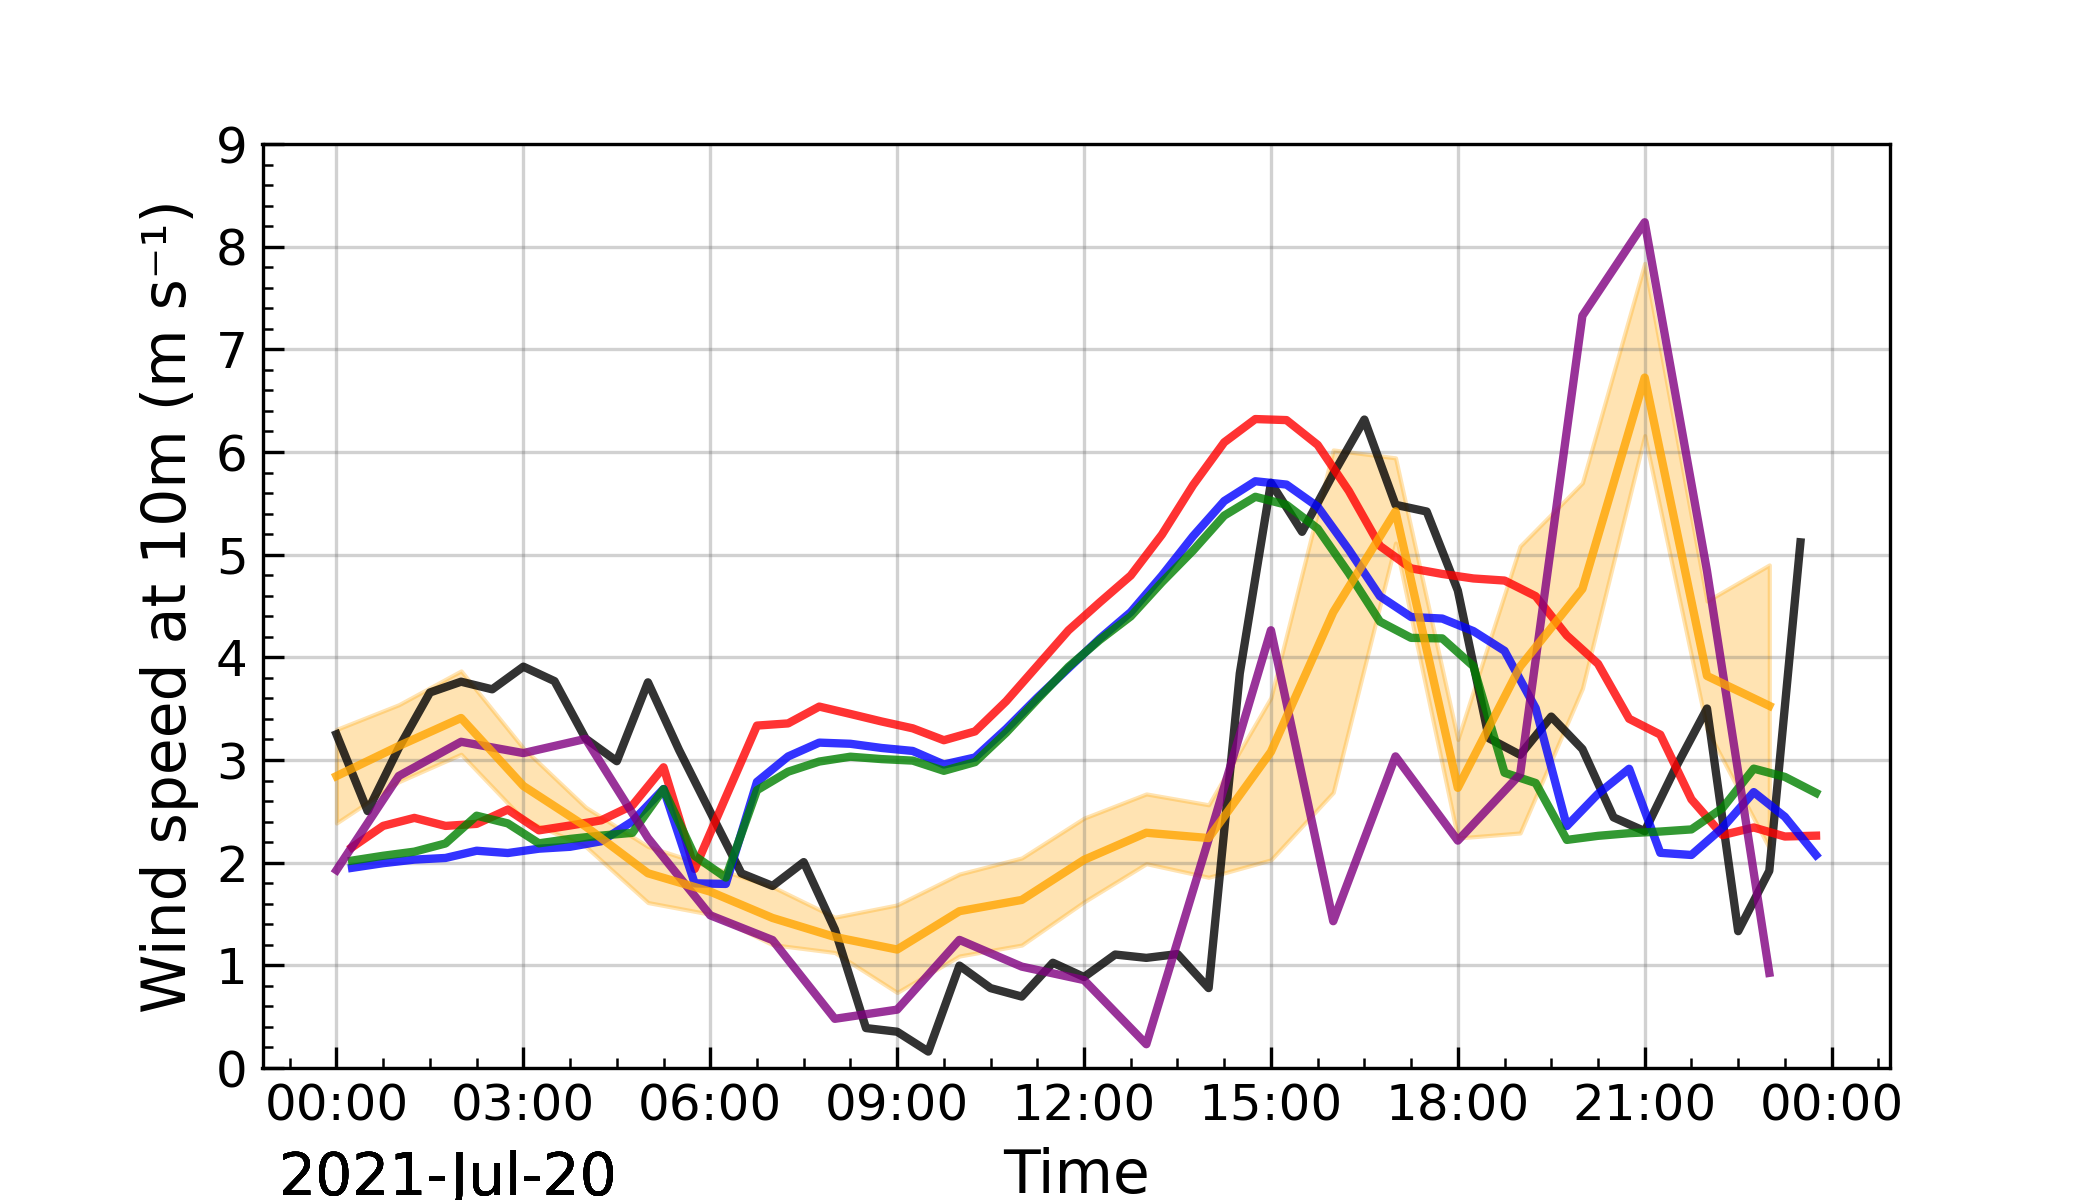
\includegraphics[width=\textwidth]{images/chap5/IOP_TS/TS_2021-07-20_cendrosa_wind_speed_10m.png}
        \end{subfigure} \\
        \begin{subfigure}[t]{0.5\textwidth}
            \caption{}
            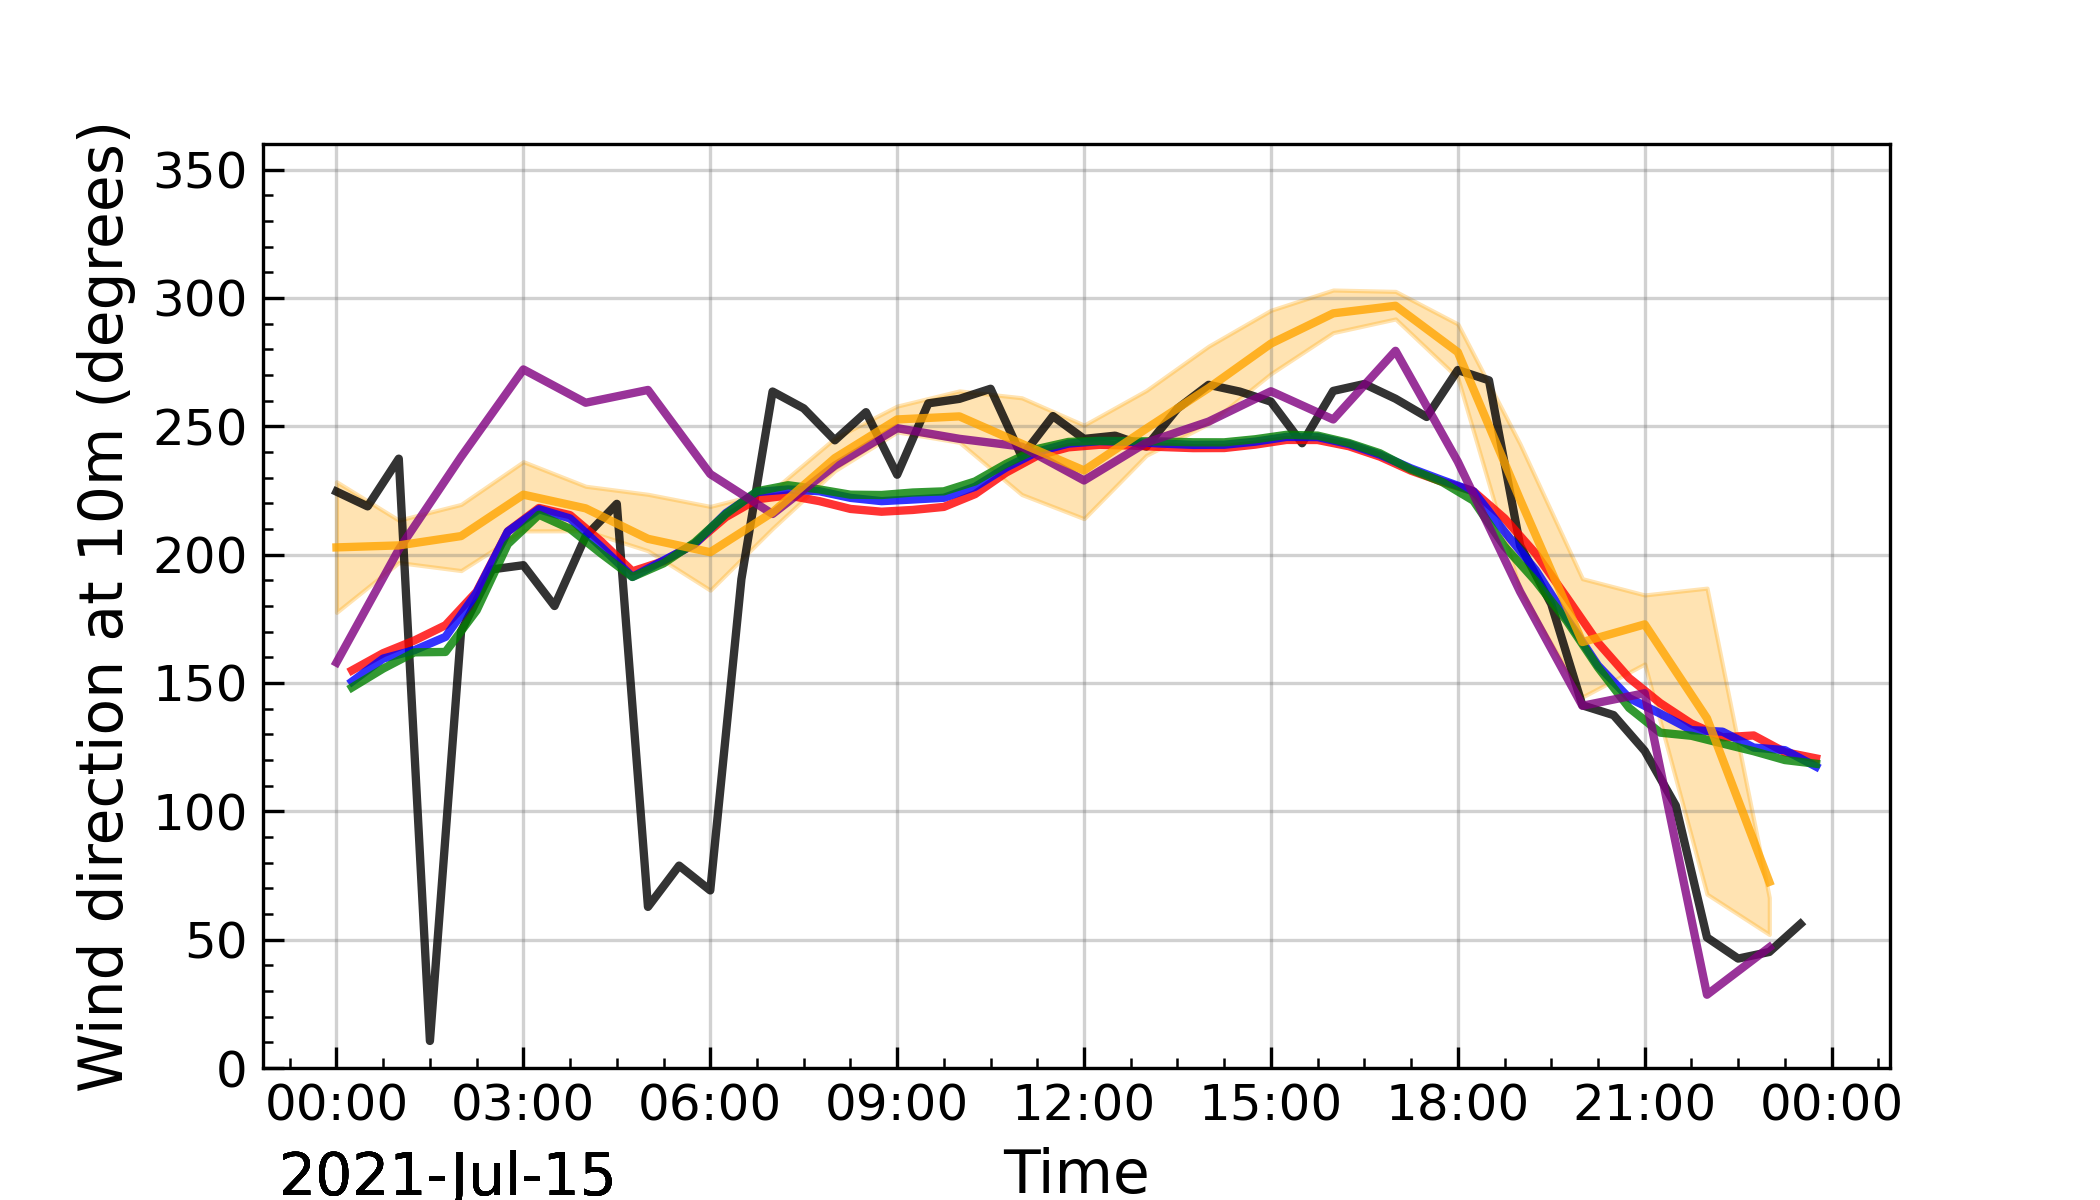
\includegraphics[width=\textwidth]{images/chap5/IOP_TS/TS_2021-07-15_cendrosa_wind_direction_10m.png}
        \end{subfigure} &
        \begin{subfigure}[t]{0.5\textwidth}
            \caption{}
            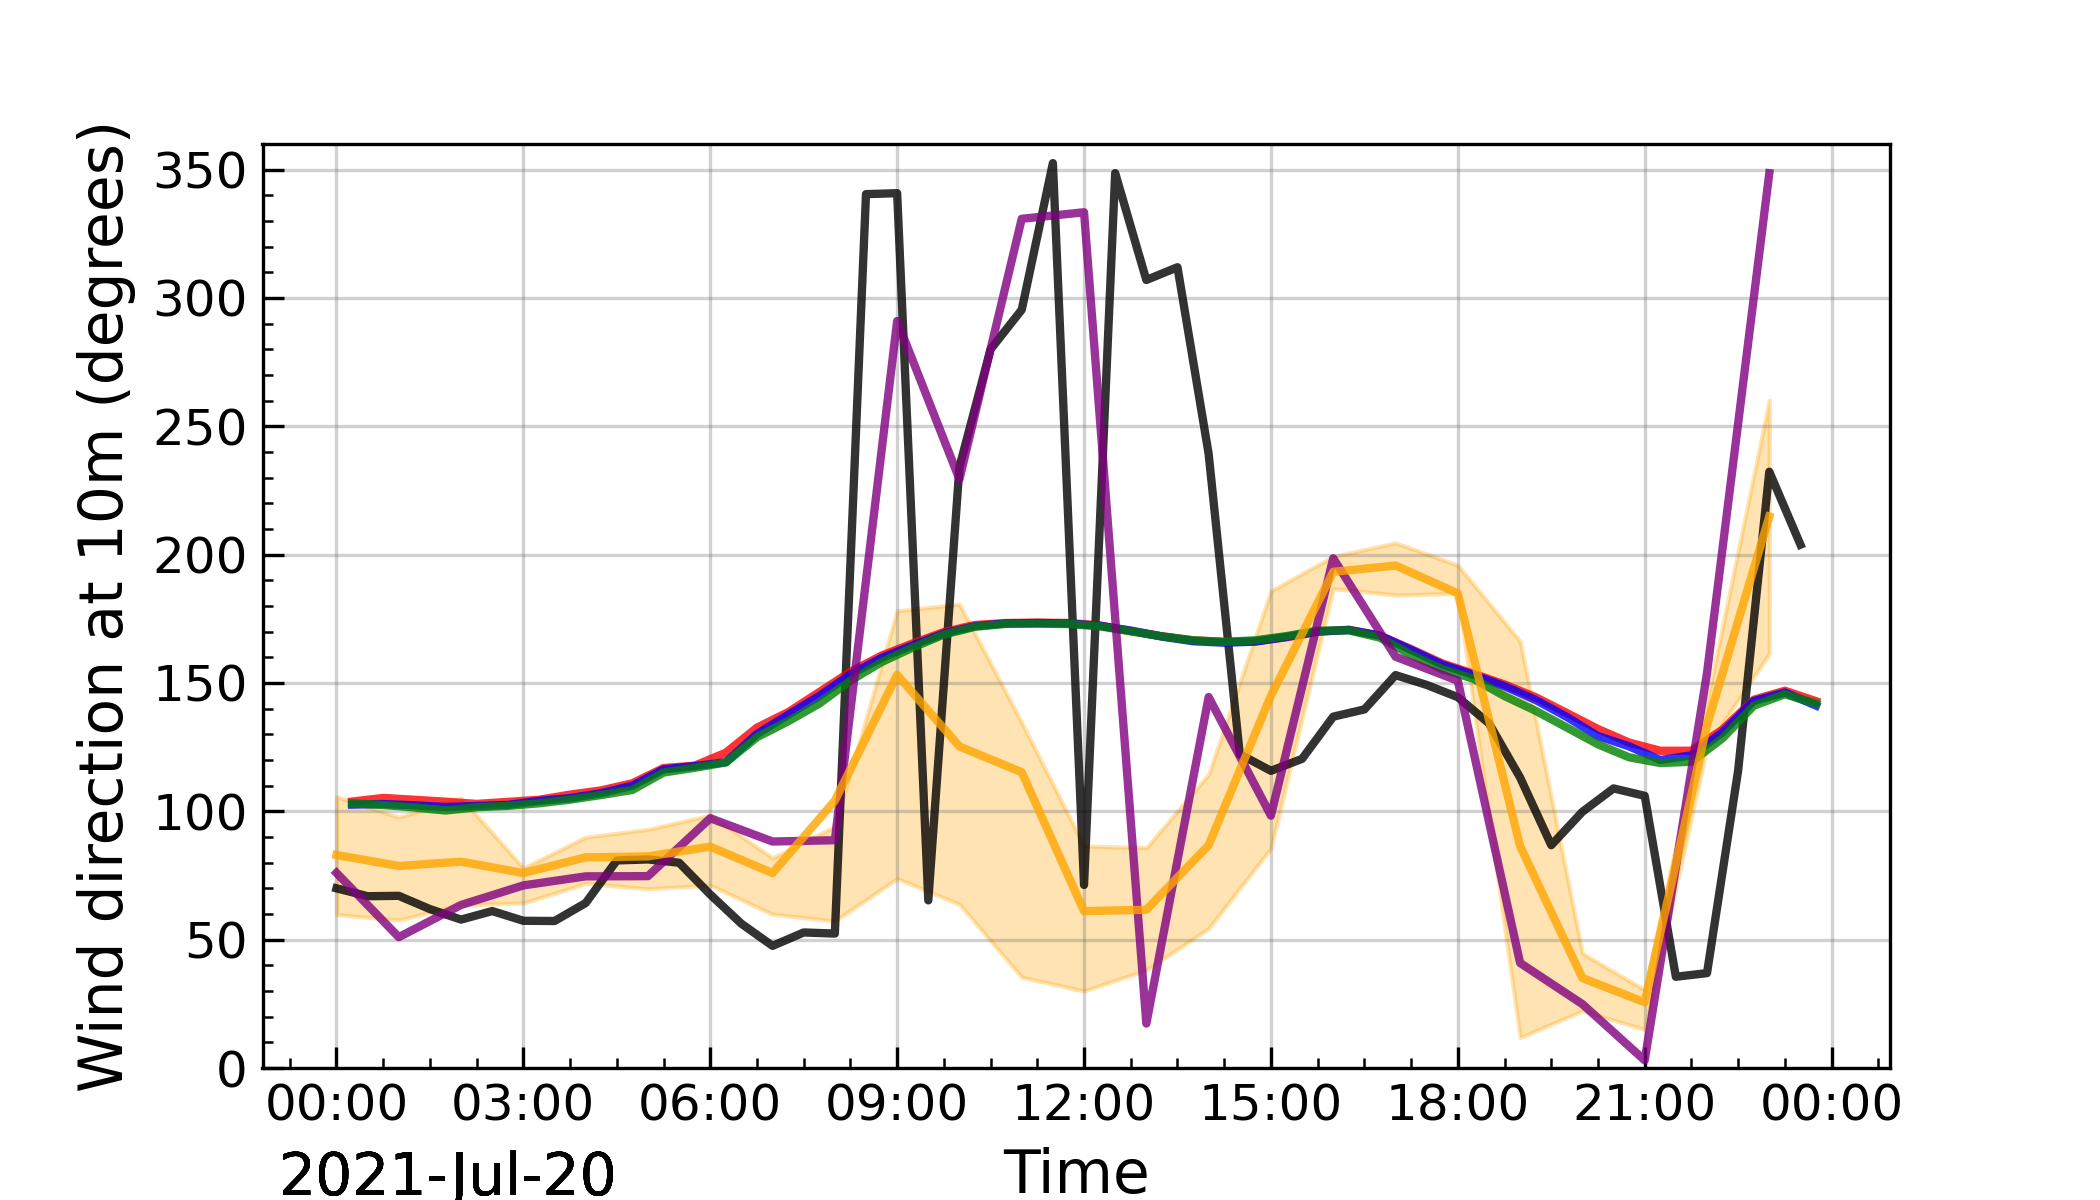
\includegraphics[width=\textwidth]{images/chap5/IOP_TS/TS_2021-07-20_cendrosa_wind_direction_10m.png}
        \end{subfigure} \\
    \end{tabular}
    \caption{}
    \label{fig:iop_days_TS_surfvars}
\end{figure}

%Fig : energy fluxes Cendrosa
\begin{figure}[hbtp]
    \centering
    \begin{tabular}{cc}
        %turb fluxes
        \begin{subfigure}[t]{0.5\textwidth}
            \caption{}
            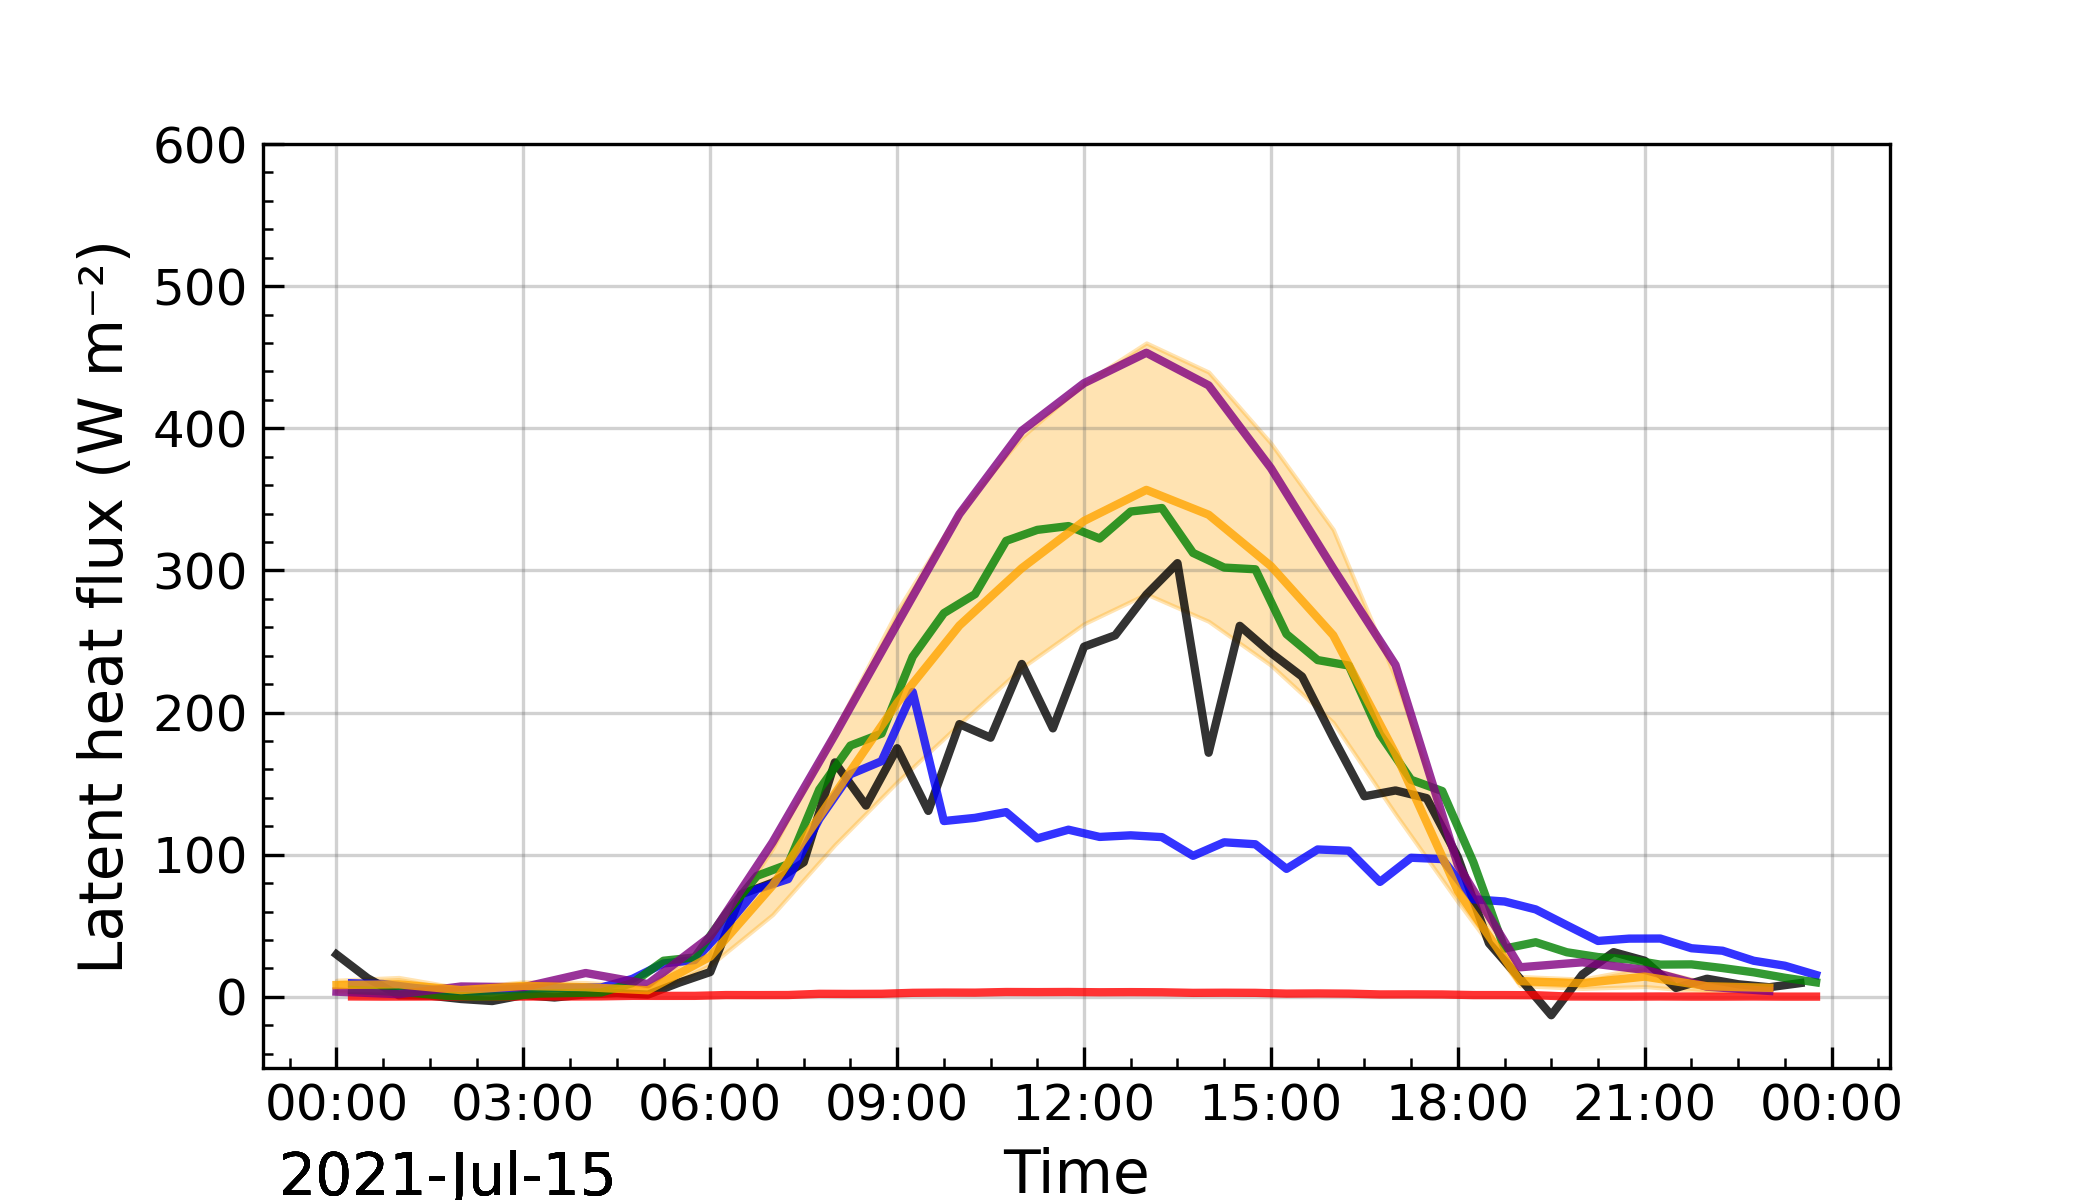
\includegraphics[width=\textwidth]{images/chap5/IOP_TS/TS_2021-07-15_cendrosa_flat.png}
        \end{subfigure} &
        \begin{subfigure}[t]{0.5\textwidth}
            \caption{}
            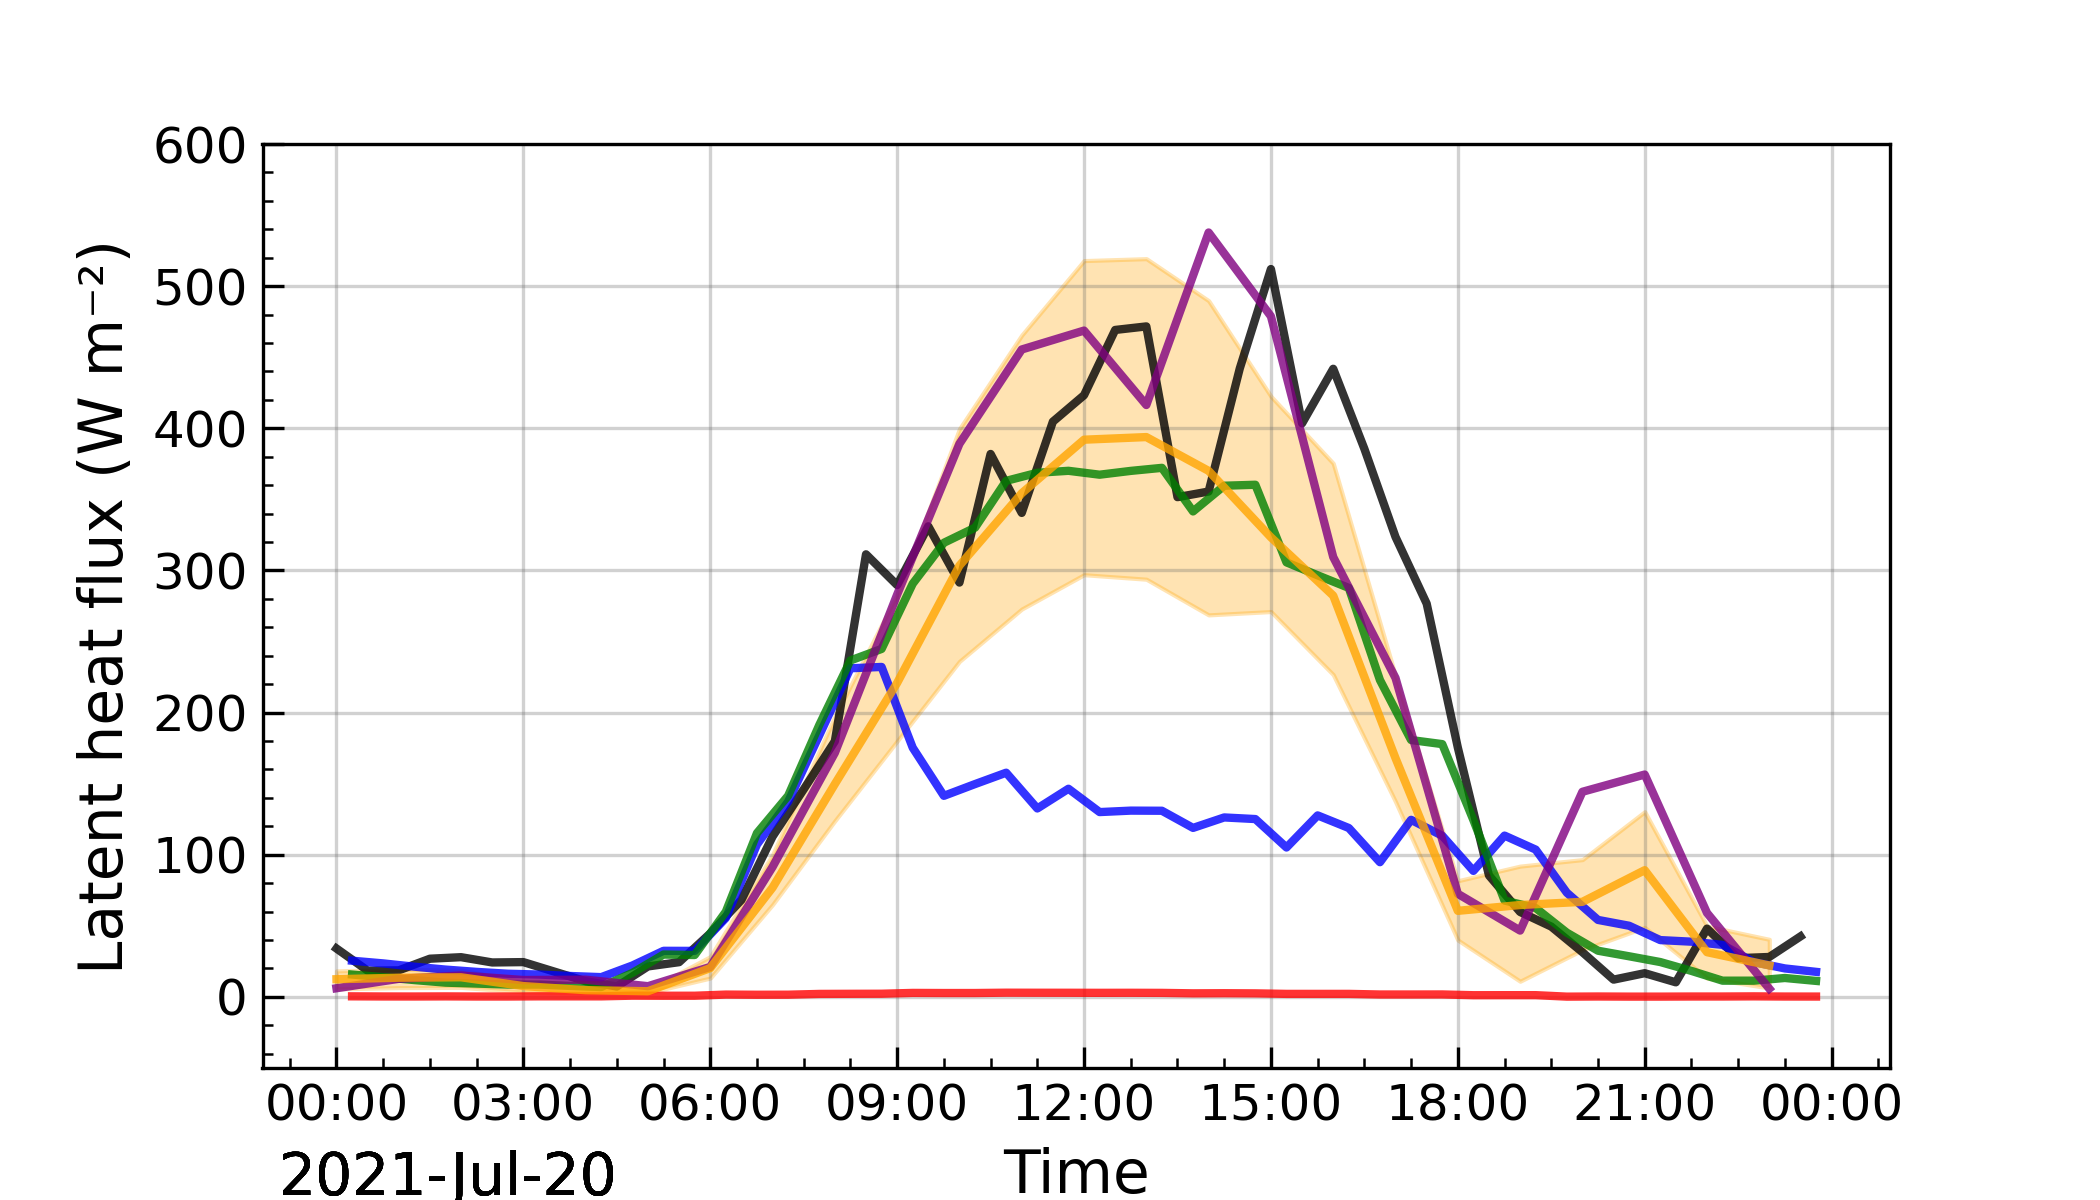
\includegraphics[width=\textwidth]{images/chap5/IOP_TS/TS_2021-07-20_cendrosa_flat.png}
        \end{subfigure} \\
        \begin{subfigure}[t]{0.5\textwidth}
            \caption{}
            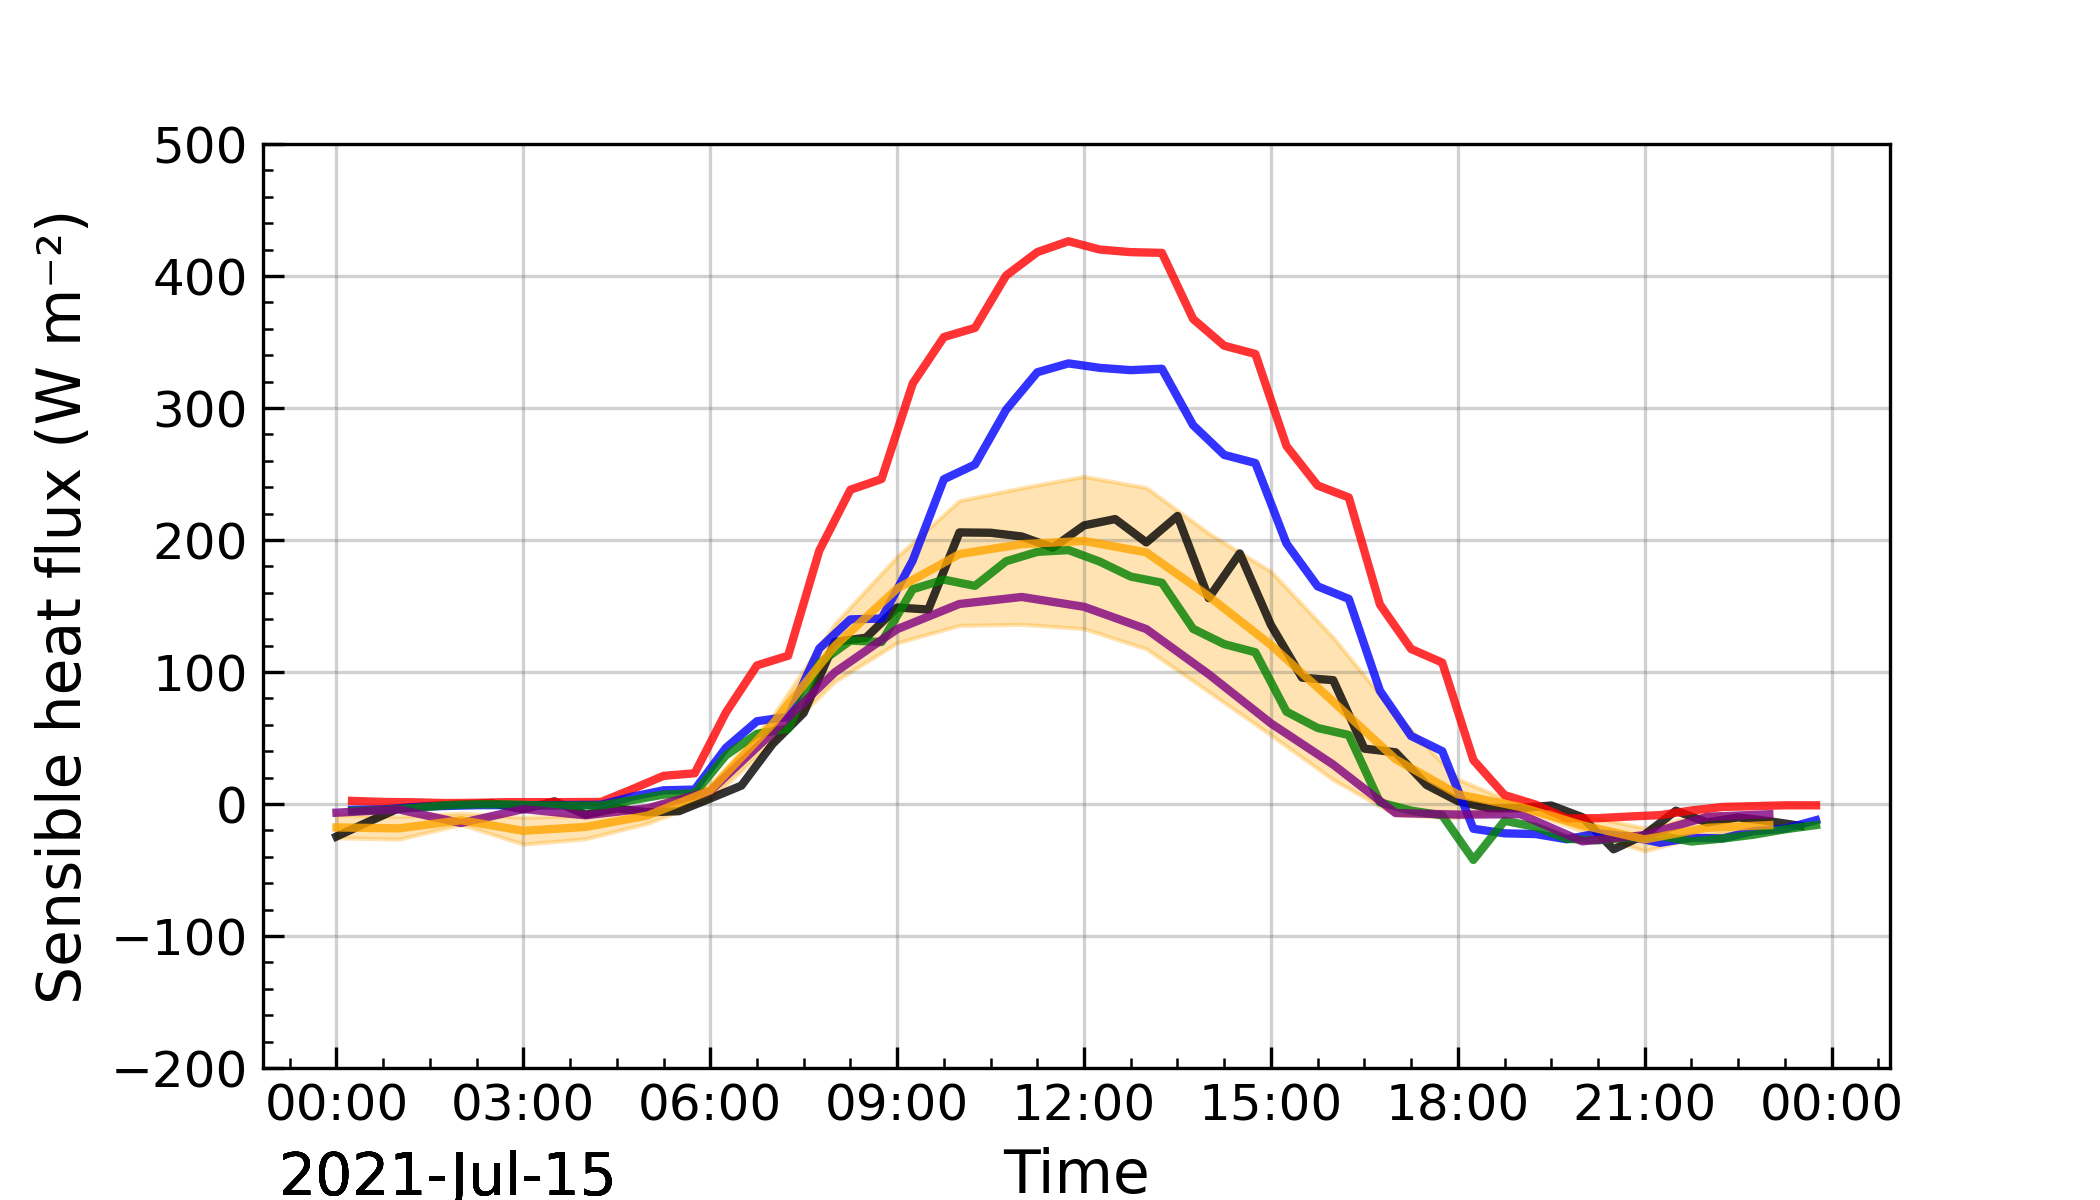
\includegraphics[width=\textwidth]{images/chap5/IOP_TS/TS_2021-07-15_cendrosa_sens.png}
        \end{subfigure} &
        \begin{subfigure}[t]{0.5\textwidth}
            \caption{}
            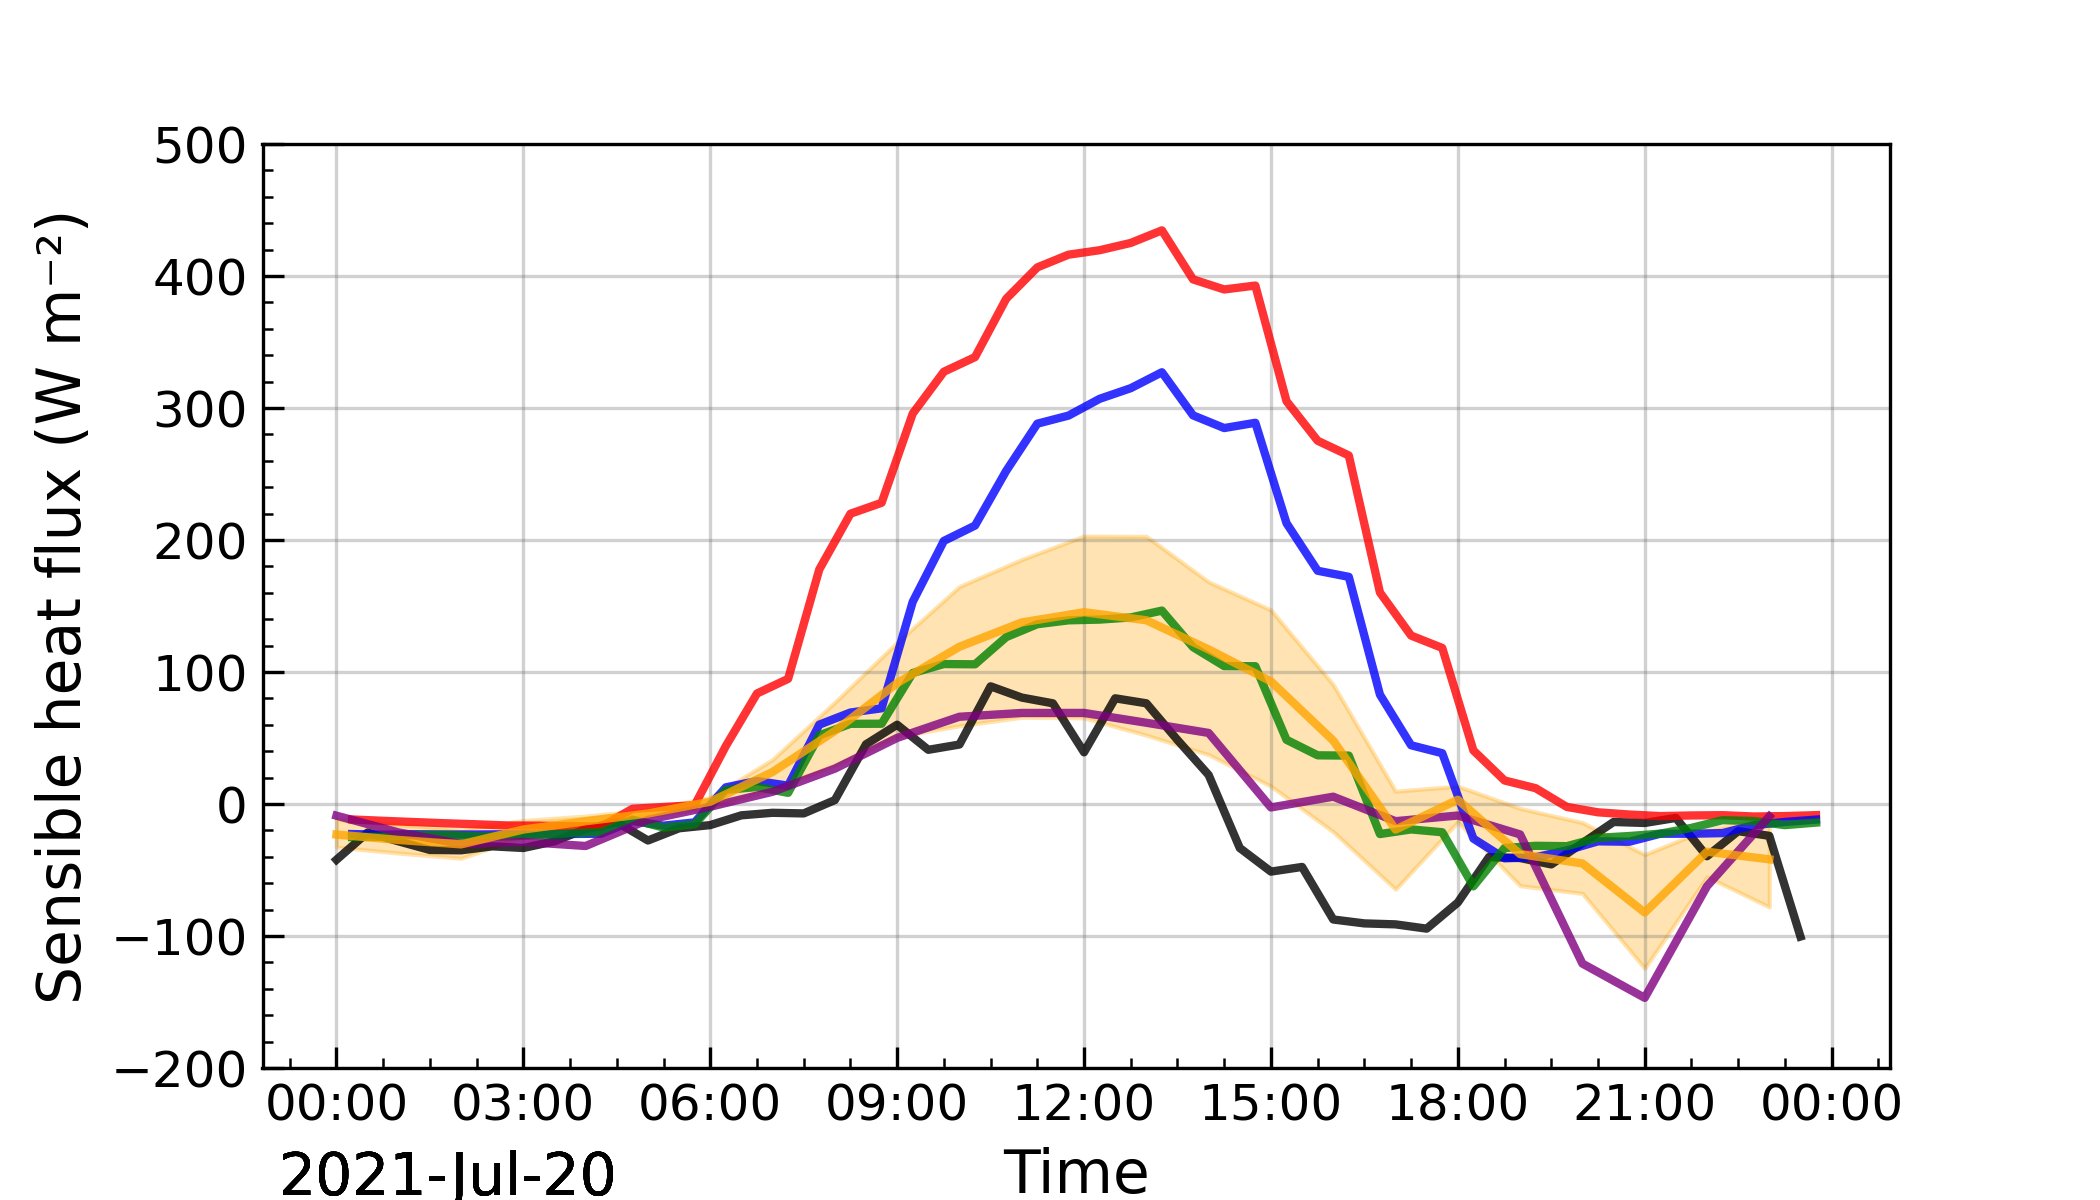
\includegraphics[width=\textwidth]{images/chap5/IOP_TS/TS_2021-07-20_cendrosa_sens.png}
        \end{subfigure} \\
        %rad fluxes
        \begin{subfigure}[t]{0.5\textwidth}
            \caption{}
            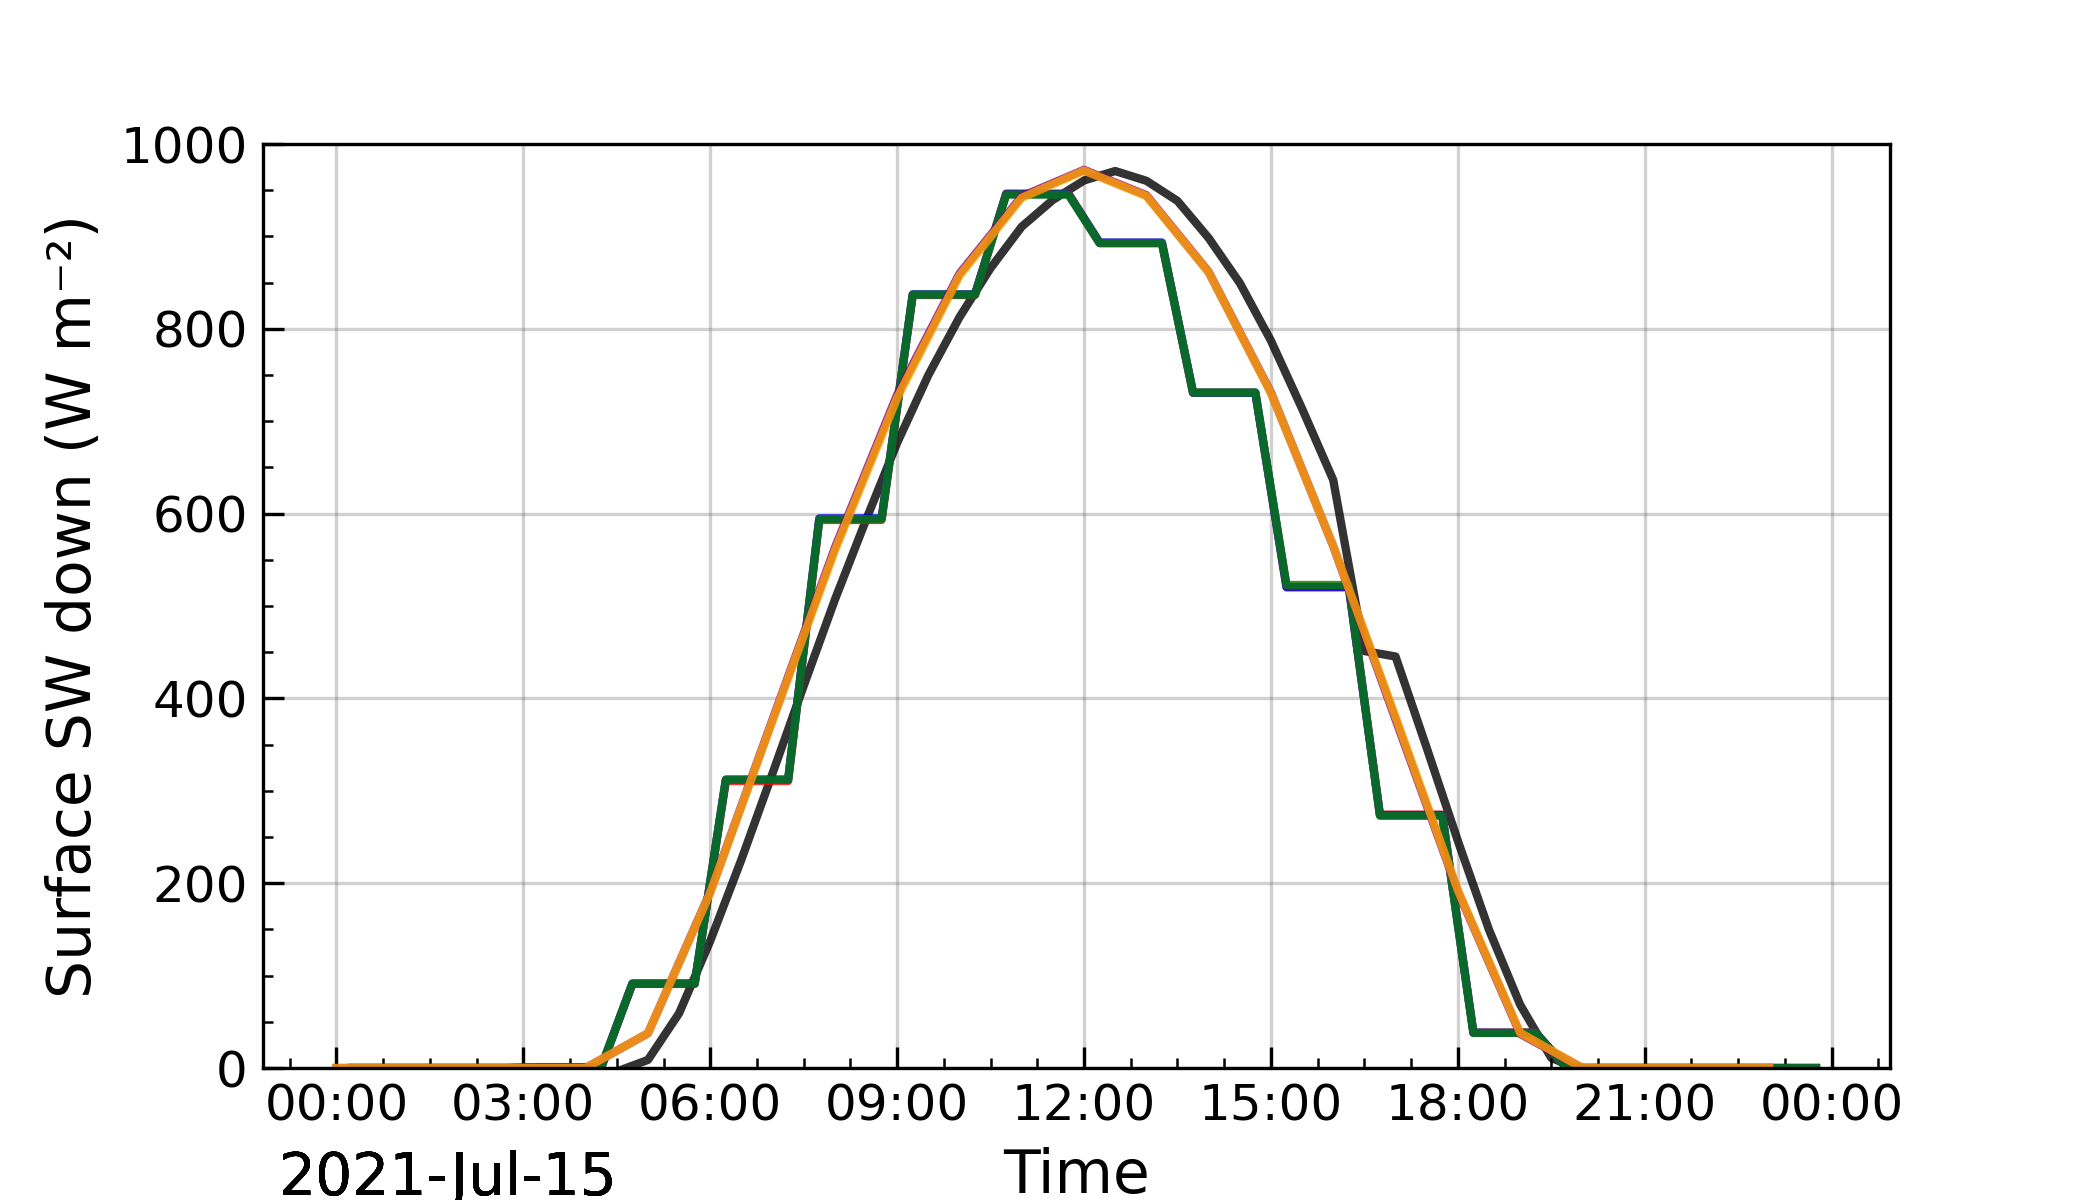
\includegraphics[width=\textwidth]{images/chap5/IOP_TS/TS_2021-07-15_cendrosa_SWdnSFC.png}
        \end{subfigure} &
        \begin{subfigure}[t]{0.5\textwidth}
            \caption{}
            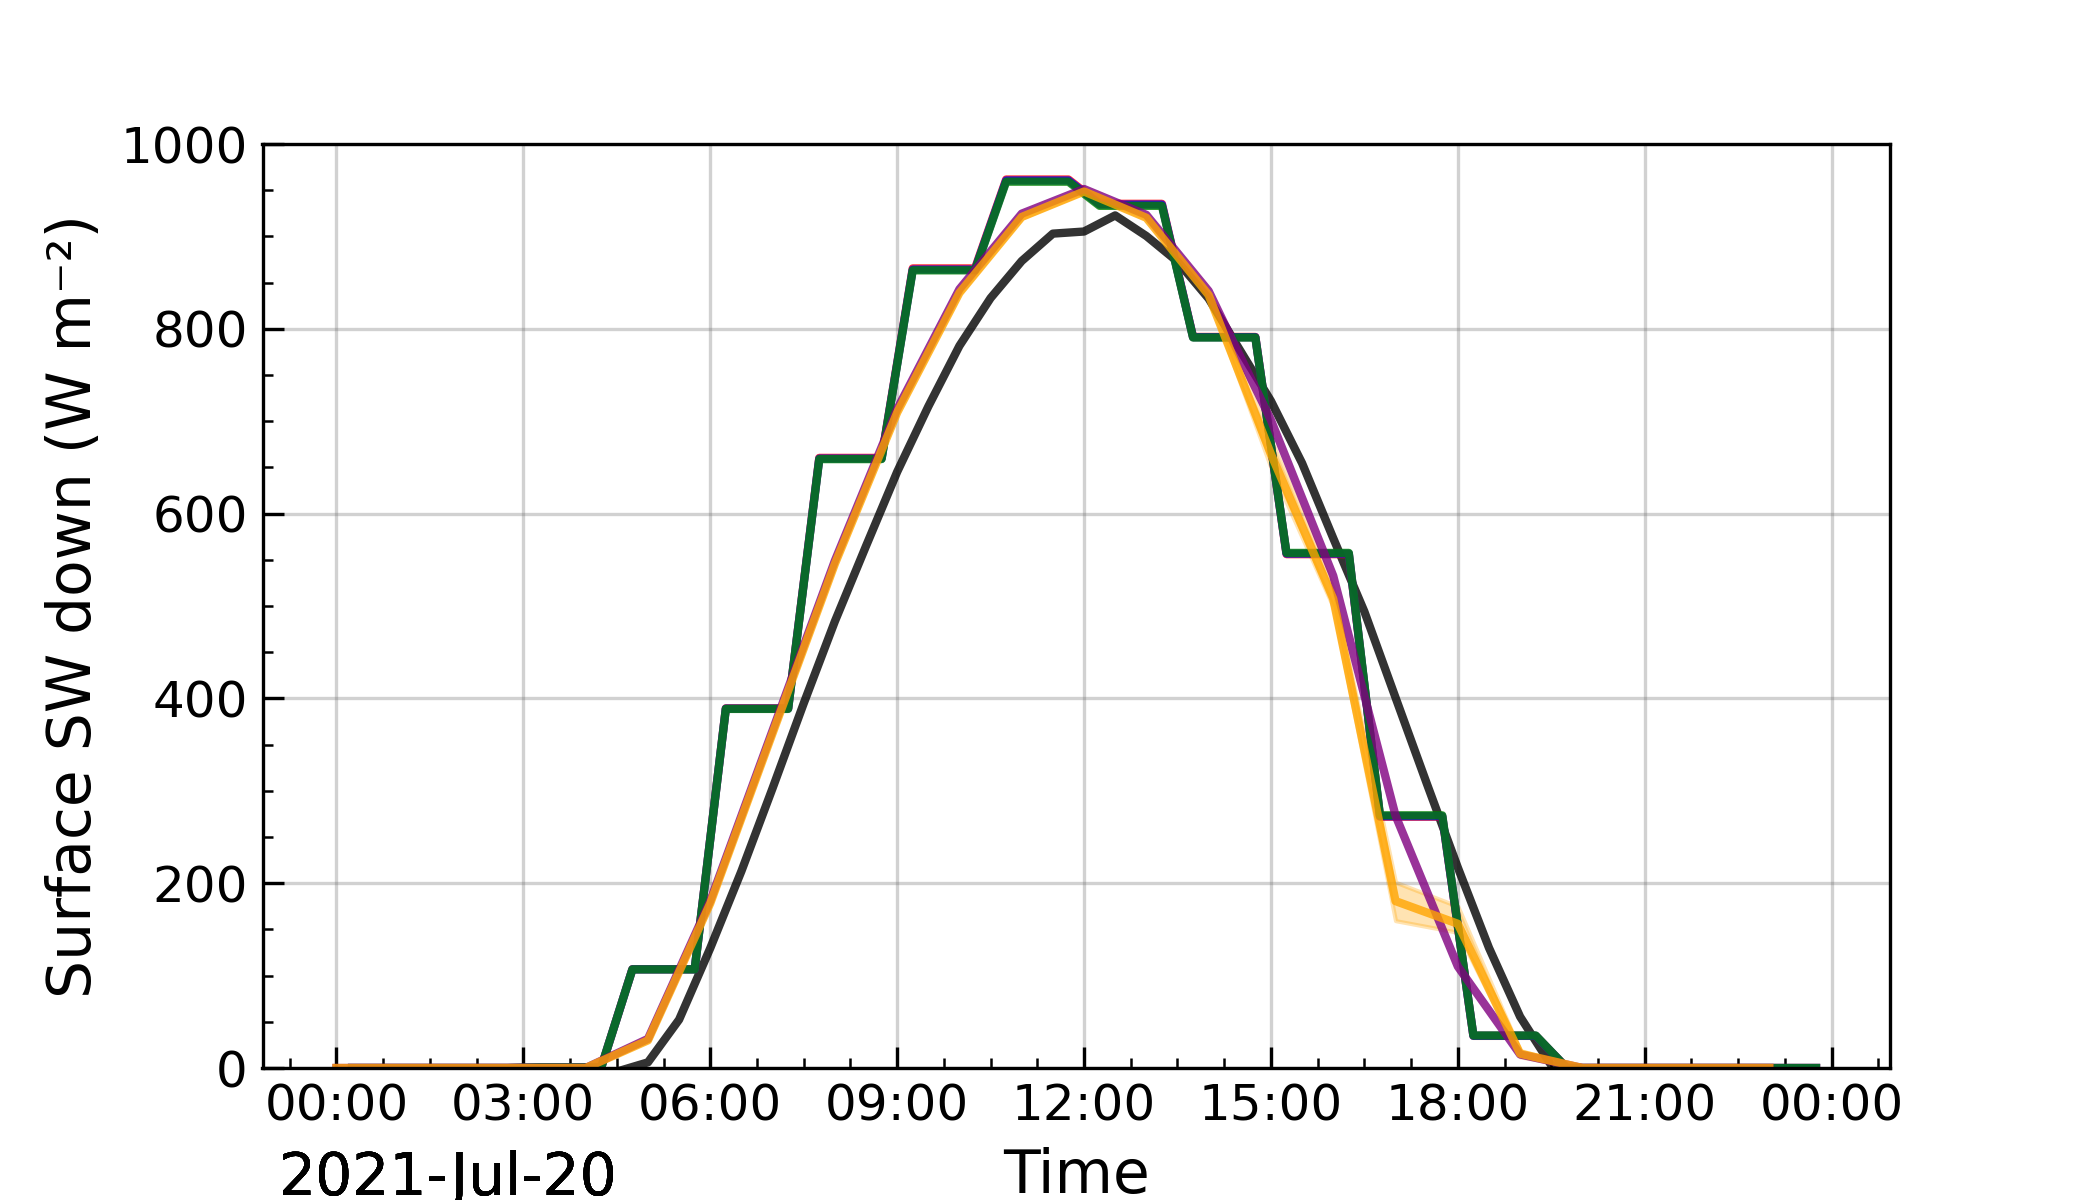
\includegraphics[width=\textwidth]{images/chap5/IOP_TS/TS_2021-07-20_cendrosa_SWdnSFC.png}
        \end{subfigure} \\
        \begin{subfigure}[t]{0.5\textwidth}
            \caption{}
            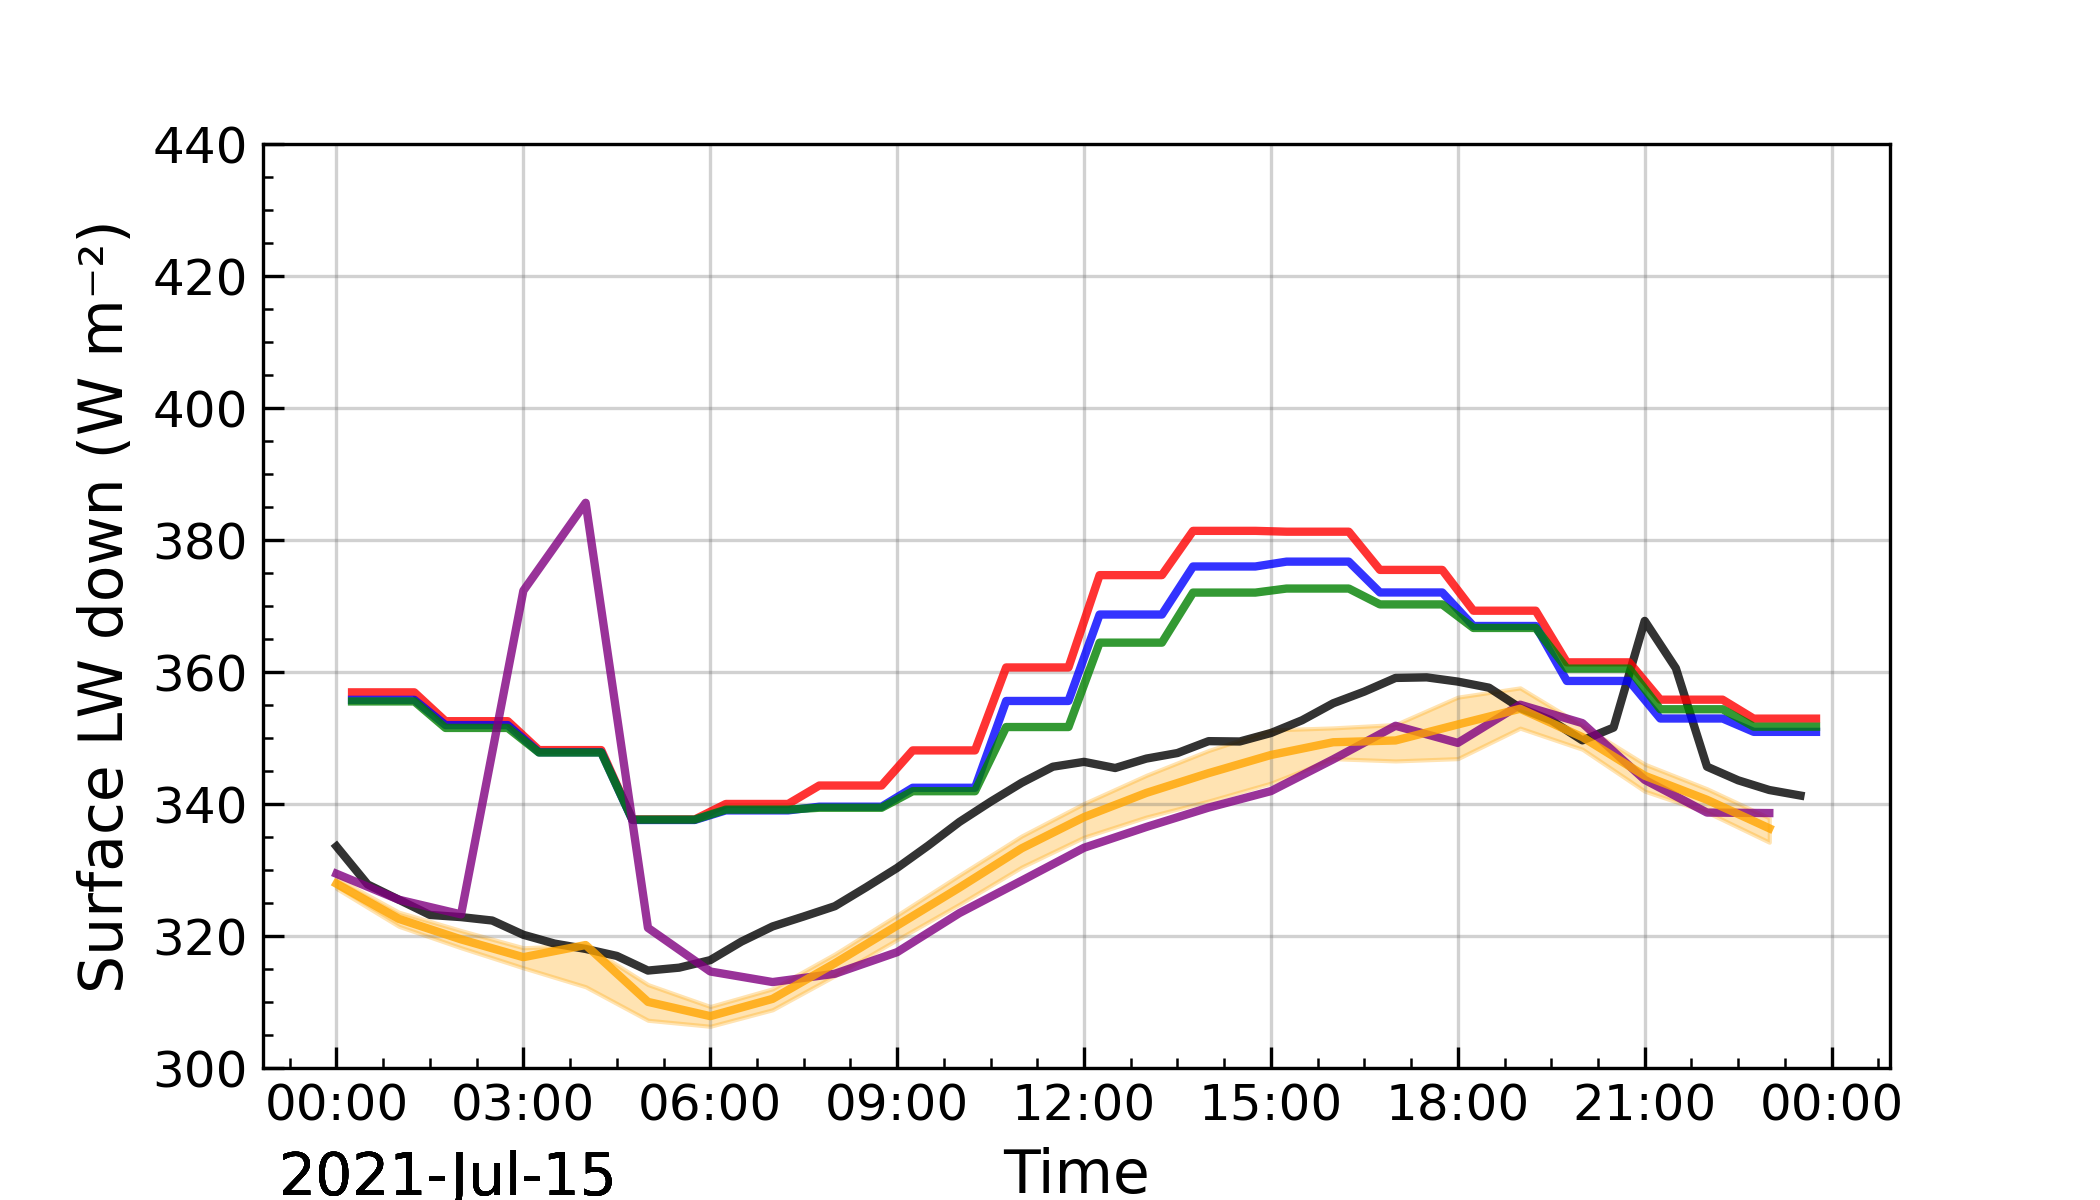
\includegraphics[width=\textwidth]{images/chap5/IOP_TS/TS_2021-07-15_cendrosa_LWdnSFC.png}
        \end{subfigure} &
        \begin{subfigure}[t]{0.5\textwidth}
            \caption{}
            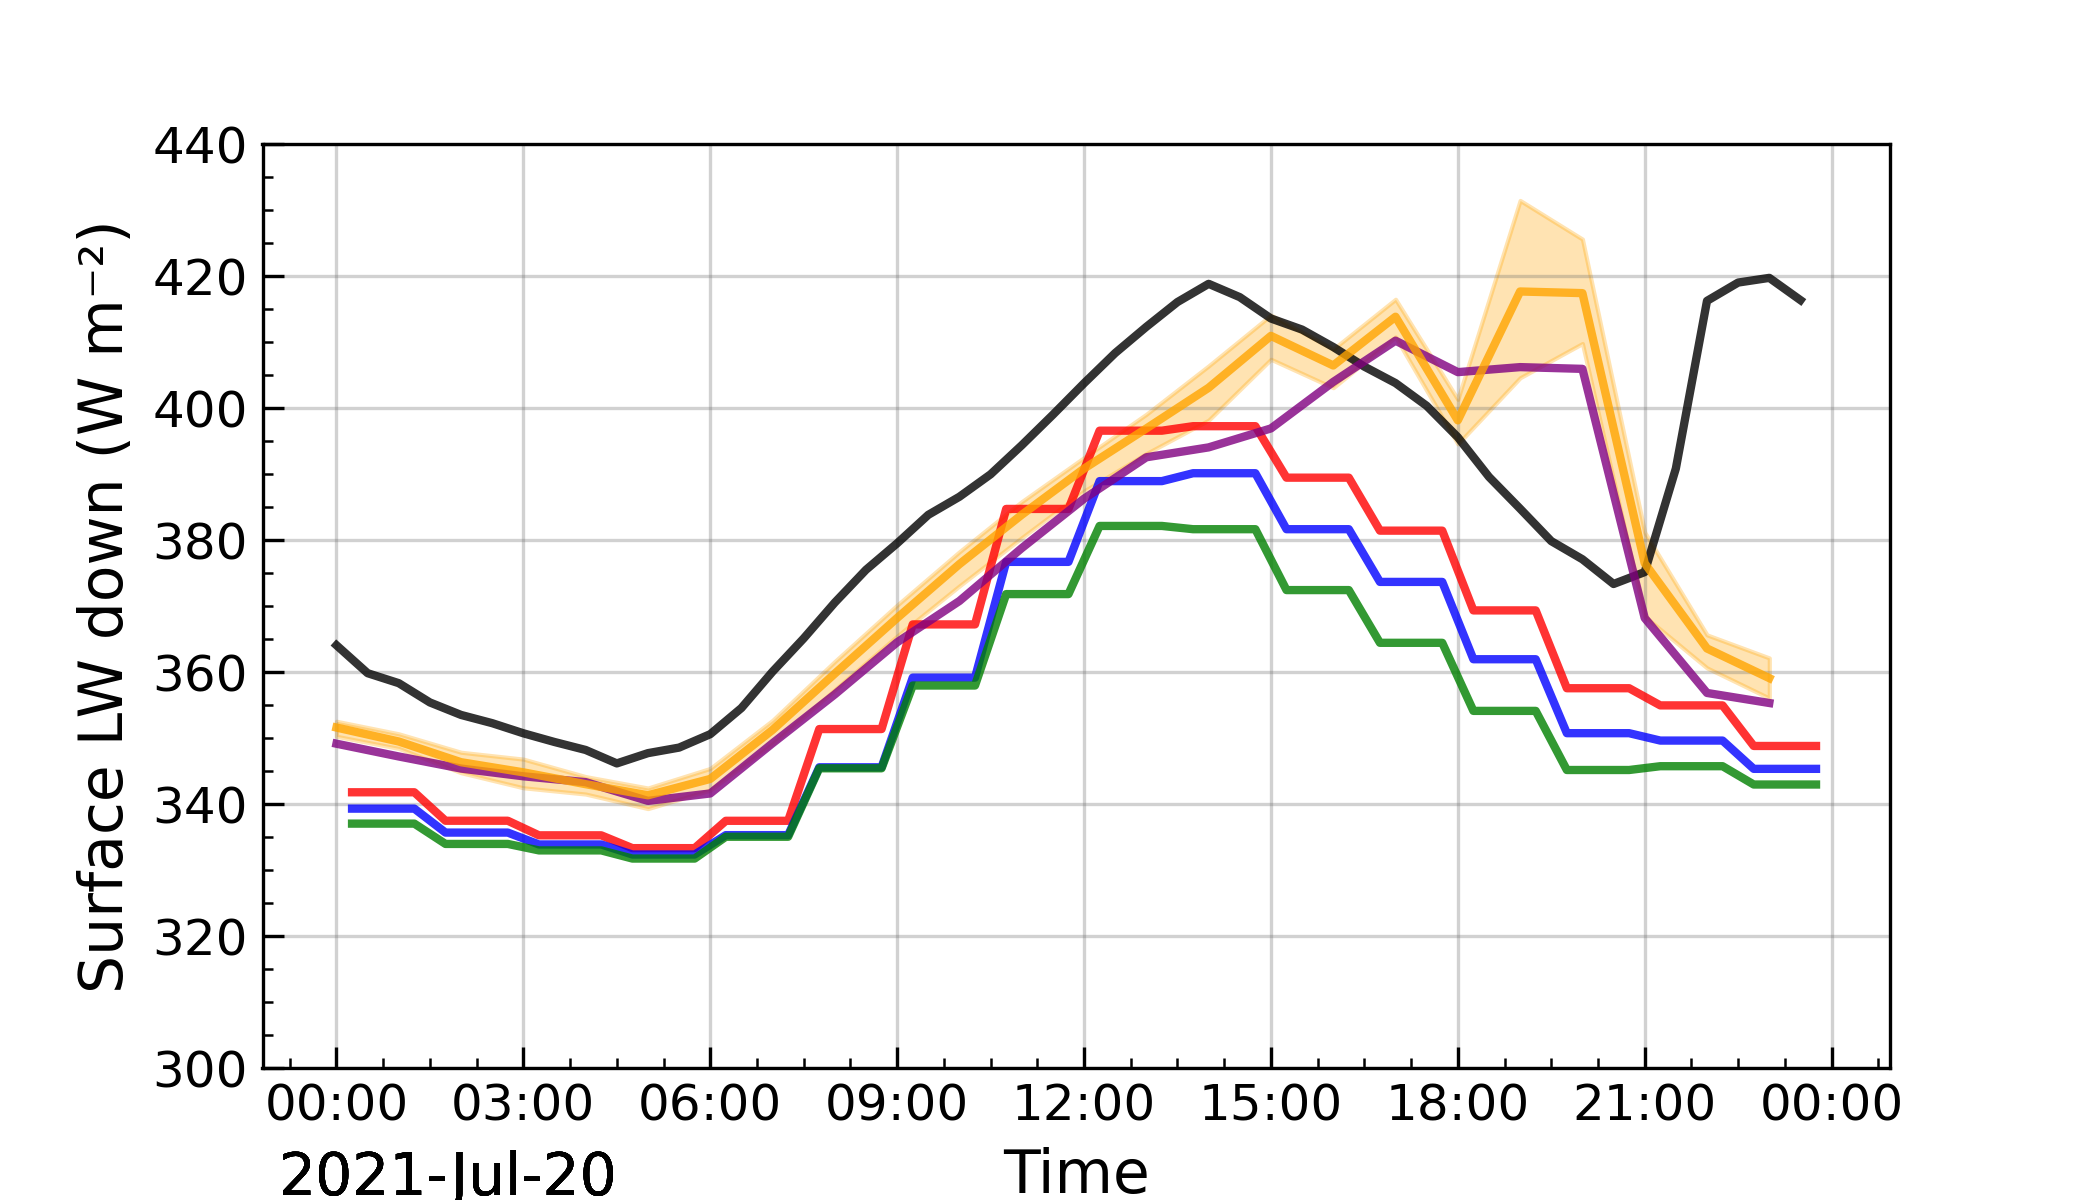
\includegraphics[width=\textwidth]{images/chap5/IOP_TS/TS_2021-07-20_cendrosa_LWdnSFC.png}
        \end{subfigure}
    \end{tabular}
    \caption{}
    \label{fig:iop_days_TS_energy}
\end{figure}

Overall, the downward longwave radiation flux (LW down, Fig. \ref{fig:iop_days_TS_energy}g-h) summarises several differences between 15 July and 20 July. 15 July has a smaller LW down flux since the atmosphere is cooler and drier, and ICOLMDZ overestimates it because of a warm bias. In \irrboost this warm bias is much smaller, but specific humidity is overestimated so overall, the bias in LW down is only slightly reduced. 
On 20 July, ICOLMDZOR presents a smaller warm bias (almost no bias for \irrboost) but a strong dry bias, leading to an underestimation of LW down. The comparison of vertical profiles to radisoundings at 12UTC  provides further insight into the behaviour of the atmosphere on these two days (Section \ref{sec:vertical_profiles}).

%todo:figure of winds at 12UTC (10m and 850hPa) ideally mesoNH and LMDZ
%todo:mention somewhere that this setup is not particularly tuned to relfect synoptic conditions, and that it's already impressive to be this much in agreement with obs and mesoMean
\clearpage

\subsection{Impact of irrigation on vertical profiles at 12UTC}
\label{sec:vertical_profiles}

%15 July
On 15 July at 12UTC, the surface warm bias seen in ICOLMDZOR seems to be present in all the ABL, where potential temperature is 5K higher than in observations for the \noirr simulation at La Cendrosa. At Els Plans, it is 4K higher, which suggests that this is not only due to a lack of ET. This is confirmed by the profile of specific humidity, since the \noirr and \irr simulations in the lower atmosphere are really close to the observations and \mesomean values.
%option:mention that above ABL, ICOLMDZOR is too moist ?
On both sites, the ABL height for \noirr and \irr is about 1700 m, which is higher than in observations (800 m at La Cendrosa, 900 at Els Plans), which can be attributed to the overestimated surface sensible heat flux (Fig. \ref{fig:iop_days_TS_energy}c,  \ref{fig:iop_days_TS_energy_elsplans}c). 
At La Cendrosa, the warm bias is reduced by 1K in the \irrboost simulation as a consequence of surface cooling, and specific humidity in the ABL increases by 1 g \perkg, beyond the observed and \mesomean value, and is similar to the \mesoexact value. 
The ABL is also clearly lowered compared to \noirr, down to 1200 m, likely through the reduction of the sensible heat flux. This is a good improvement of the structure, but still about 250 m higher than the average ABL height seen in \mesomean, showing that over a grid cell, a good representation of the average surface fluxes does not fully translate into a good average ABL structure.
Among the causes of such discrepancies in vertical structure are the subgrid heterogeneities (discussed in Section \ref{sec:heterogeneities}), and variables which are mostly determined by the dynamics. The vertical profiles of wind show that the direction simulated by ICOLMDZOR is correct, but that wind speed might be too low over most of the ABL, on both sites. Although the \mesomean and \mesoexact profiles are closer to ICOLMDZOR than observations, they still show more variations, which might influence mixing in the lower atmosphere and the position of the ABL top. %à compléter, creuser ?

\hfill

%20 July
Compared to the observed profile on 20 July at 12UTC, the \noirr simulation still presents a warm bias of 2K in potential temperature and a dry bias of 1t o 1.5 g \perkg in the ABL at La Cendrosa, whereas at Els Plans there is no bias in potential temperature but a dry bias of 2.5 g \perkg in specific humidity. 
The ABL height in \noirr is 1200 m at La Cendrosa whereas in the radiosounding, although it remains subject to interpretation, it is more likely around 1400 m, and in Meso-NH it is slightly above 1500 m.
At Els Plans, the observed profile is easier to interpret with a clear inversion at 1500 m, which is located higher in Meso-NH (around 1650 m) and much lower in ICOLMDZOR simulations (around 850 m). 
This is all the more surprising since surface sensible heat flux is higher than observations in ICOLMDZOR simulations (even \irrboost at La Cendrosa), suggesting that the extent of the ABL in ICOLMDZOR is mostly dominated by other factors. %todo:get more insight from FredHo or Etienne
In particular, the wind speed at La Cendrosa is two to three times higher in ICOLDMZOR than the observed one in the first 500 m of the atmosphere (and this is the case throughout all morning).%todo:link to appendix fig
It is similar at Els Plans until 11UTC, but at 12UTC (shown here), a strong southeasterly wind is observed up to 800 m, and although the direction is rather correct in ICOLMDZOR and Meso-NH, the rapid increase in wind speed is not captured.

In this context, the irrigation at La Cendrosa enables a large improvements of the warm and dry biases in \irrboost. Potential temperature is decreased by 1K, while all the mixed layer benefits from the surface moistening, allowing specific humidity to match the radiosounding profile. 
At La Cendrosa, there seems to be an internal sublayer up to 500 m, cooler than the rest of the mixed layer. It is also visible in the Meso-NH simulation, where it is also moister, but this type of process is unsurprisingly not captured by ICOLMDZOR, and potential temperature is matches observations better between 500 m and 900 m.
The performance is not as satisfying regarding ABL structure however since the height of the mixed layer is clearly reduced to 900 m in \irrboost, worsening the limitation identified in \noirr. 

%Els Plans : moister than La Cendrosa : advection process ?

\hfill

The first takeaway from this analysis of vertical profiles is that the impact of irrigation in \irrboost is not limited to surface turbulent fluxes or 2-meter temperature and specific humidity, but also impacts to the atmospheric boundary layer.

This allows irrigation to improve the warm bias in the ABL on both days, reducing potential temperature by 1K. 
On 15 July, three elements suggest that the 5K bias is not only due to local processes: 2-m temperature is not completely corrected in \irrboost even though latent heat flux is overestimated, the warm bias is also very present at Els Plans and specific humidity is rather correct on both sites. Therefore, it is not very surprising that the impact of irrigation, through the surface energy budget, is not sufficient to reduce all the bias in the ABL. 
On 20 July however, 2-meter temperature matches observations and \mesomean really well in \irrboost and potential temperature simulated by ICOLMDZOR is in good agreement with observations at Els Plans, the specific humidity in the ABL matches the radiosounding at 12UTC, although it is still underestimated at 2-meter. This suggests that the temperature bias is mostly due to local processes and a lack of soil moisture in \noirr, which is why it is largely reduced in the ABL over La Cendrosa.
%option : It can be noted here that on this day, Meso-NH seems to underestimate temperature
In ICOLMDZOR, the impact of irrigation on potential temperature and specific humidity in the ABL is similar for the two days considered in absolute value, but the relevance compared to existing biases of ICOLMDZOR depends on the situation.
Regarding ABL height, the same conclusion can be made, on 15 July where ABL height was inisitally too high, irrigation lowers it by 400 m, making it much closer to the \mesomean value, but on the 20th it is lowered by 300 m even though it was already lower than observations and Meso-NH.

In general, the impacts on wind speed and direction is quite negligible, except for wind speed around 1000 m above ground level at La Cendrosa on 20 July, where it follows the top of the boundary layer.
The impacts on the Els Plans site are also very small, apart from a small moistening (at most 0.5 g \perkg) of the ABL, visible on both days, which is made possible by advection of moister air from neighbouring irrigated grid cells.

To further investigate the mixing in the ABL and underestand what control its vertical extension, the influence of subgrid heterogeneities was explored.
The main objective was to determine whether the average surface flux approach used in ICOLDMZOR was relevant to realistically propagate impacts of irrigation in the ABL, or if major drivers of ABL development were missed by not accounting for subgrid flux heterogeneities. 

%Fig : profiles 1507 12UTC
\begin{figure}[hbtp]
    \centering
    \makebox[\textwidth][c]{%
    \begin{tabular}{@{}cccc@{}}
        %cendrosa
        \begin{subfigure}[t]{0.382\textwidth}
            \caption{}
            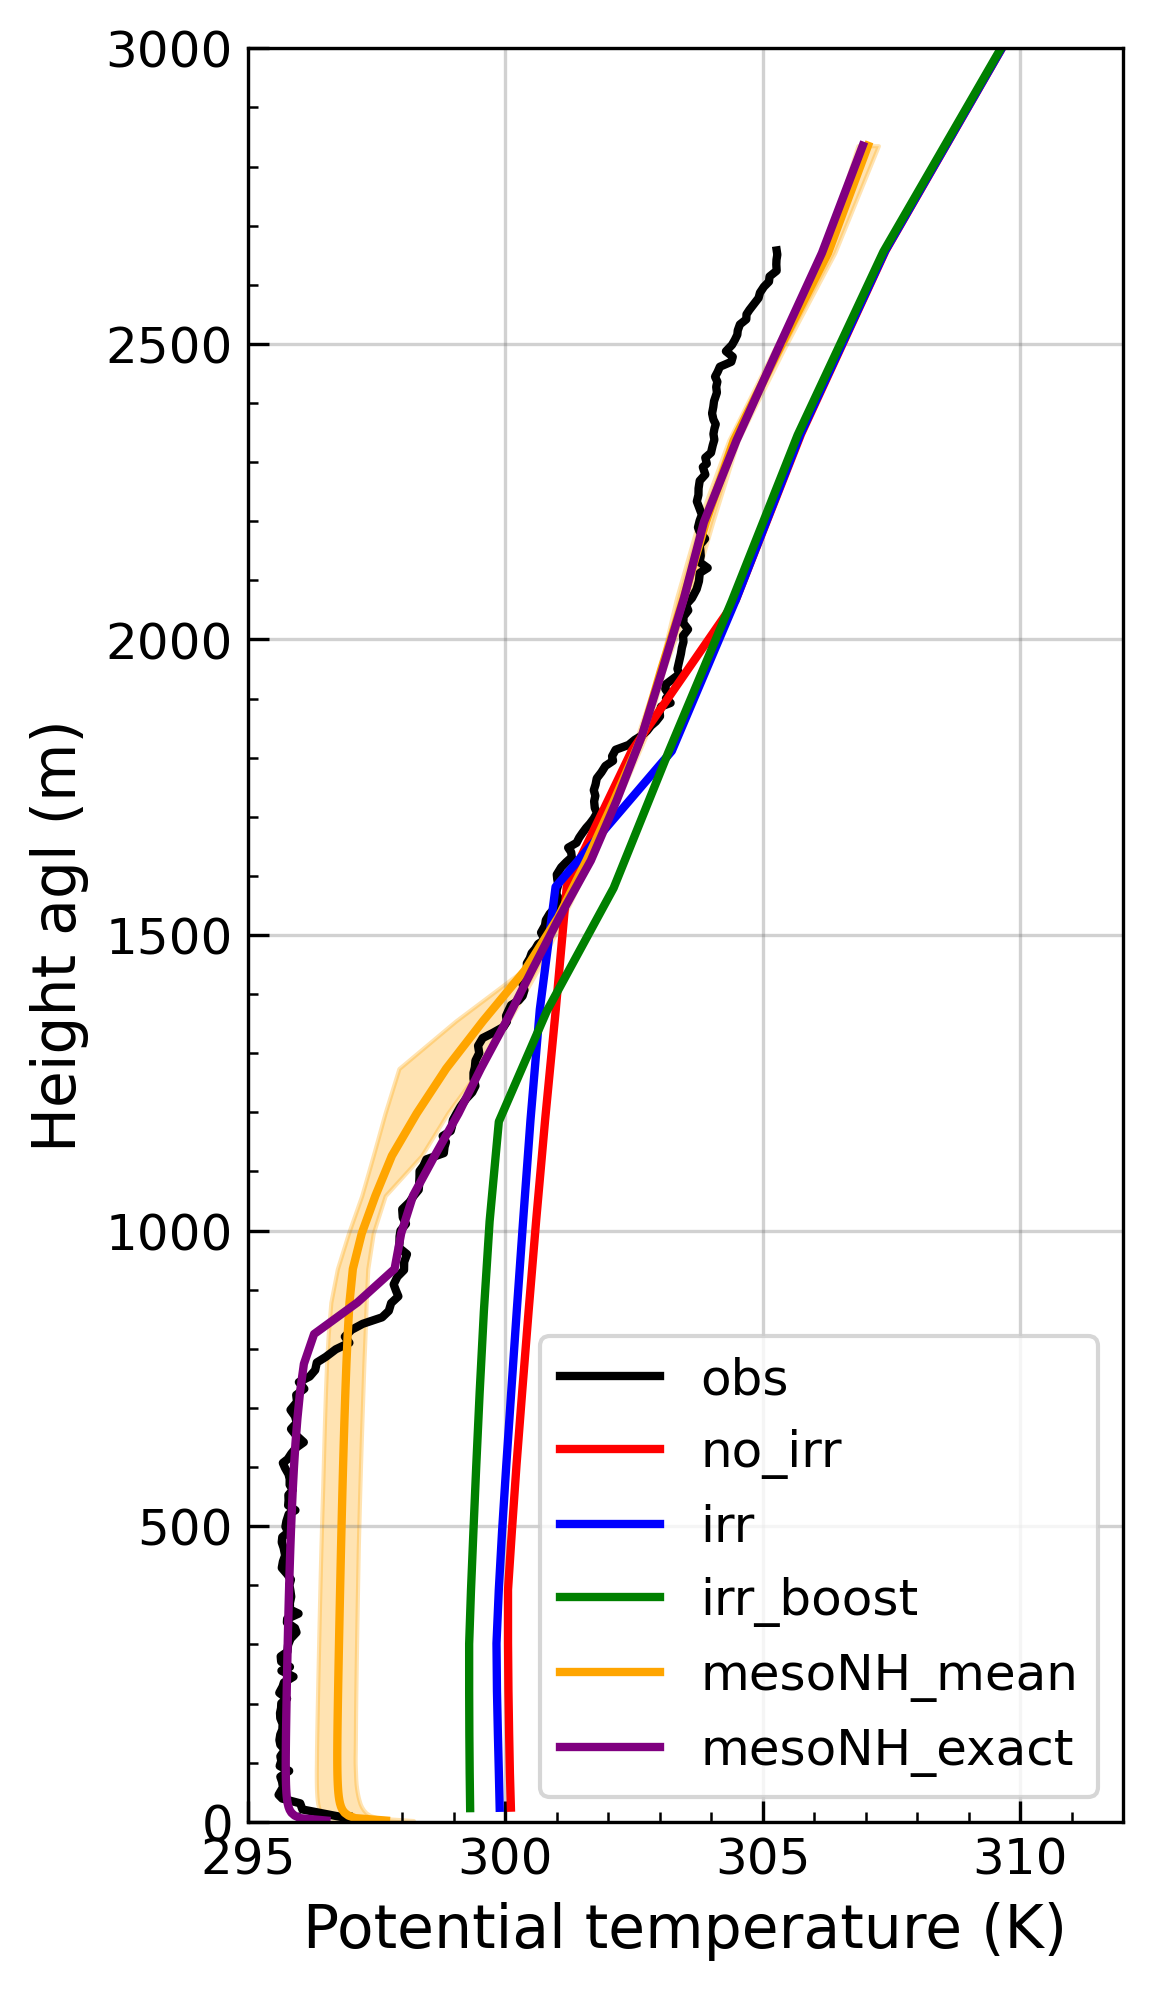
\includegraphics[width=\textwidth]{images/chap5/profiles/profile_cendrosa_theta_1507_.png}
        \end{subfigure} &
        \begin{subfigure}[t]{0.289\textwidth}
            \caption{}
            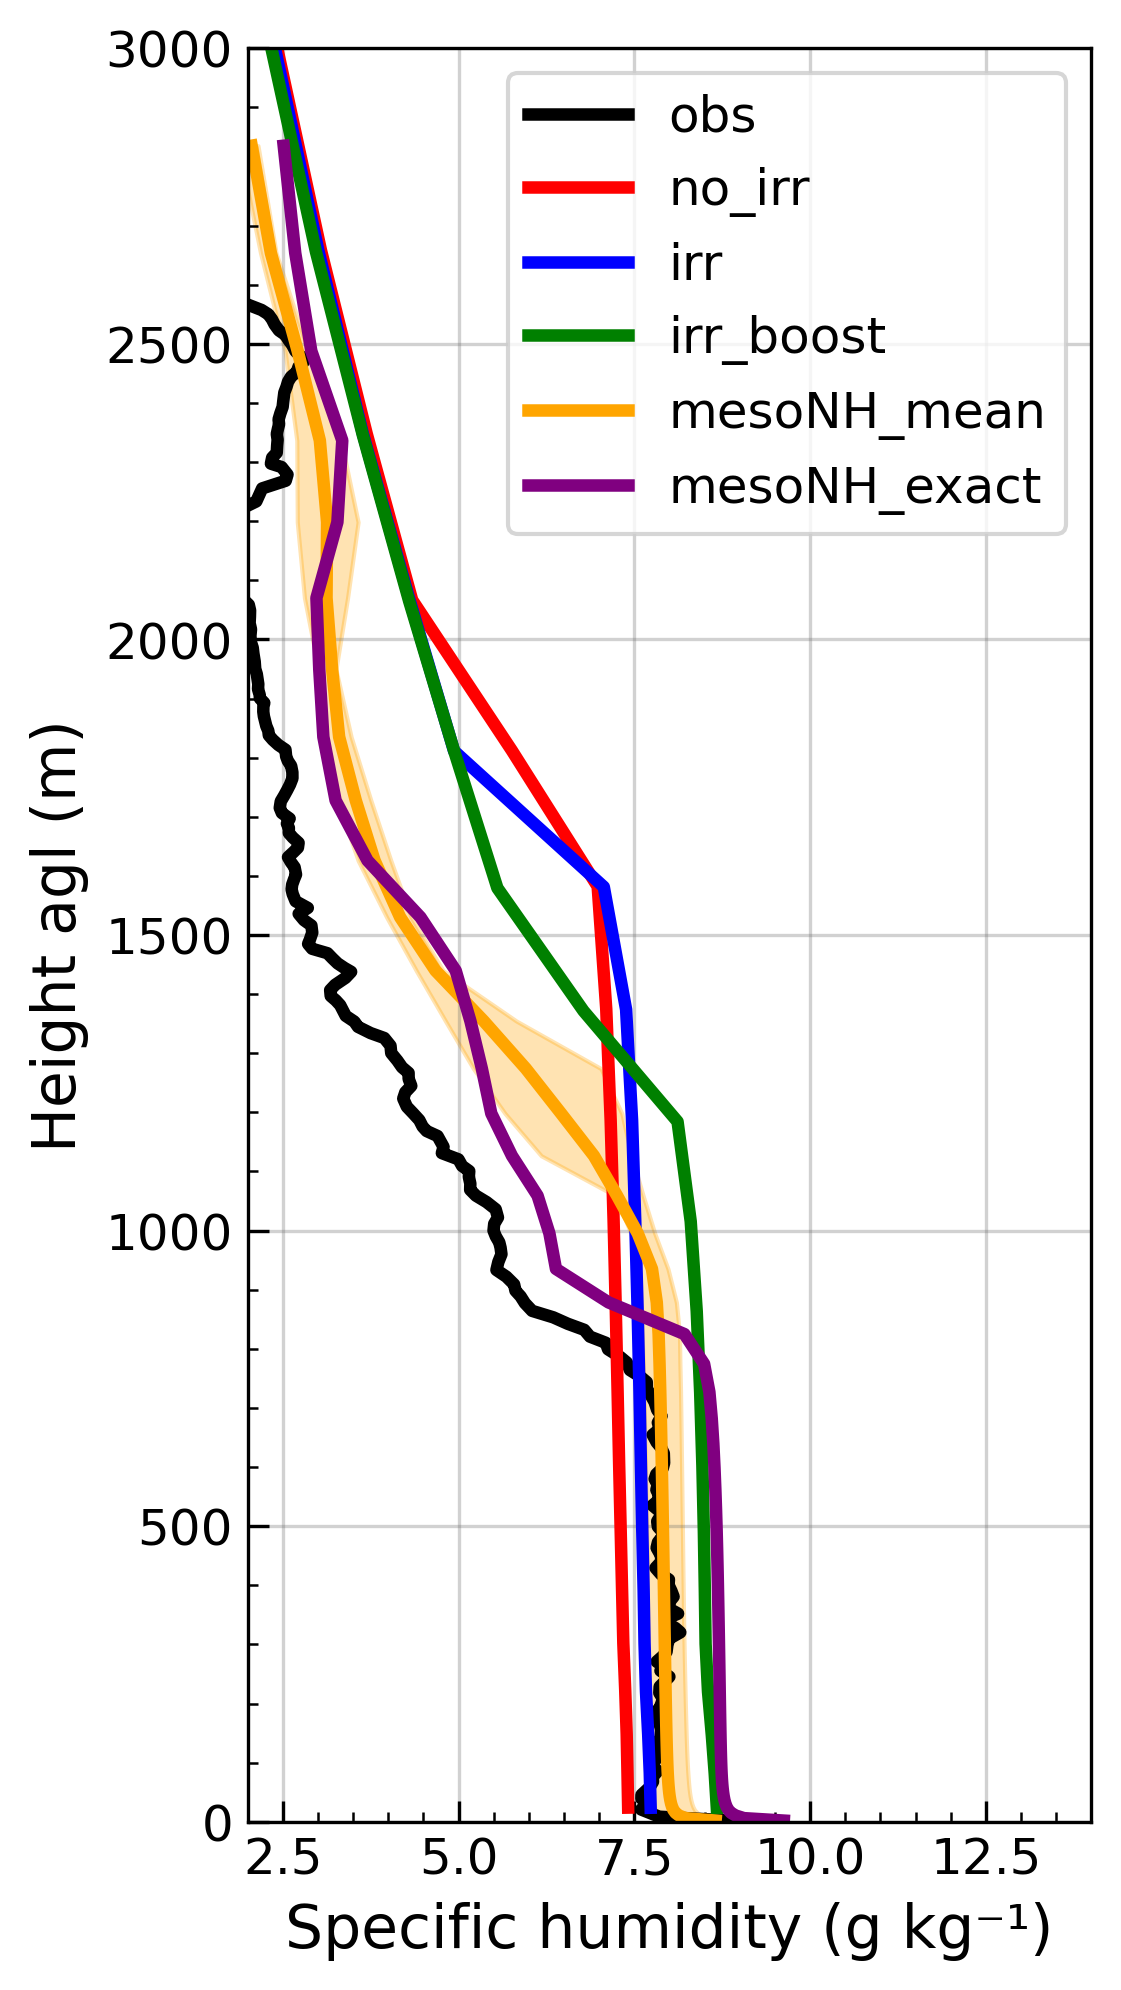
\includegraphics[width=\textwidth]{images/chap5/profiles/profile_cendrosa_ovap_1507_.png}
        \end{subfigure} &
        \begin{subfigure}[t]{0.283\textwidth}
            \caption{}
            \includegraphics[width=\textwidth]{images/chap5/profiles/profile_cendrosa_wind_speed_1507_.png}
        \end{subfigure} &
        \begin{subfigure}[t]{0.283\textwidth}
            \caption{}
            \includegraphics[width=\textwidth]{images/chap5/profiles/profile_cendrosa_wind_direction_1507_.png}
        \end{subfigure} \\
        %elsplans
        \begin{subfigure}[t]{0.382\textwidth}
            \caption{}
            \includegraphics[width=\textwidth]{images/chap5/profiles/profile_elsplans_theta_1507_.png}
        \end{subfigure} &
        \begin{subfigure}[t]{0.289\textwidth}
            \caption{}
            \includegraphics[width=\textwidth]{images/chap5/profiles/profile_elsplans_ovap_1507_.png}
        \end{subfigure} &
        \begin{subfigure}[t]{0.283\textwidth}
            \caption{}
            \includegraphics[width=\textwidth]{images/chap5/profiles/profile_elsplans_wind_speed_1507_.png}
        \end{subfigure} &
        \begin{subfigure}[t]{0.283\textwidth}
            \caption{}
            \includegraphics[width=\textwidth]{images/chap5/profiles/profile_elsplans_wind_direction_1507_.png}
        \end{subfigure} \\
    \end{tabular}
    }
    \caption{Vertical profiles at 12UTC on 15 July, at La Cendrosa (a-d) and Els Plans (e-h).}
    \label{fig:profiles_cendrosa_1507}
\end{figure}

%Fig : profiles 2007 12UTC
\begin{figure}[hbtp]
    \centering
    \makebox[\textwidth][c]{%
    \begin{tabular}{@{}cccc@{}}
        %cendrosa
        \begin{subfigure}[t]{0.382\textwidth}
            \caption{}
            \includegraphics[width=\textwidth]{images/chap5/profiles/profile_cendrosa_theta_2007_.png}
        \end{subfigure} &
        \begin{subfigure}[t]{0.289\textwidth}
            \caption{}
            \includegraphics[width=\textwidth]{images/chap5/profiles/profile_cendrosa_ovap_2007_.png}
        \end{subfigure} &
        \begin{subfigure}[t]{0.283\textwidth}
            \caption{}
            \includegraphics[width=\textwidth]{images/chap5/profiles/profile_cendrosa_wind_speed_2007_.png}
        \end{subfigure} &
        \begin{subfigure}[t]{0.283\textwidth}
            \caption{}
            \includegraphics[width=\textwidth]{images/chap5/profiles/profile_cendrosa_wind_direction_2007_.png}
        \end{subfigure} \\
        %elsplans
        \begin{subfigure}[t]{0.382\textwidth}
            \caption{}
            \includegraphics[width=\textwidth]{images/chap5/profiles/profile_elsplans_theta_2007_.png}
        \end{subfigure} &
        \begin{subfigure}[t]{0.289\textwidth}
            \caption{}
            \includegraphics[width=\textwidth]{images/chap5/profiles/profile_elsplans_ovap_2007_.png}
        \end{subfigure} &
        %winds
        \begin{subfigure}[t]{0.283\textwidth}
            \caption{}
            \includegraphics[width=\textwidth]{images/chap5/profiles/profile_elsplans_wind_speed_2007_.png}
        \end{subfigure} &
        \begin{subfigure}[t]{0.283\textwidth}
            \caption{}
            \includegraphics[width=\textwidth]{images/chap5/profiles/profile_elsplans_wind_direction_2007_.png}
        \end{subfigure} \\
    \end{tabular}
    }
    \caption{Vertical profiles at 12UTC on 20 July, at La Cendrosa (a-d) and Els Plans (e-h).}
    \label{fig:profiles_cendrosa_2007}
\end{figure}

\clearpage

\subsection{Importance of surface fluxes heterogeneities}
\label{sec:heterogeneities}
\clearpage

\section{Chapter conclusions}
%irrigation without boost does not have very significant impact
%with boostirr, manage to get much closer to observations 

%no impact on Els Plans site, not a surprise


%discussion
% flat in irrboost is mostly driven by bare soil evap : realistic ? error compensation? need further developments in plant behaviour ?
%irrboost very simplified test, setup not good for dynamical effects, very strong irrig for some grid cells and no irrig at Els Plans
%setup does not allow a study of heterogeneity at Els Plans but it was not the main aim here, it rather serves as a reference for noirr case
%how much of the positive impacts of irrigation are error compensation ?


\clearpage

\section{Chapter appendix}

\begin{figure}[hbtp]
    \centering
    \begin{tabular}{cc}
        \begin{subfigure}[t]{0.5\textwidth}
            \caption{}
            \includegraphics[width=\textwidth]{images/chap5/SOP_TS_DC/time_series_cendrosa_SWdnSFC.png}
        \end{subfigure} &
        \begin{subfigure}[t]{0.5\textwidth}
            \caption{}
            \includegraphics[width=\textwidth]{images/chap5/SOP_TS_DC/diurnal_cycle_cendrosa_SWdnSFC.png}
        \end{subfigure} \\
        
        \begin{subfigure}[t]{0.5\textwidth}
            \caption{}
            \includegraphics[width=\textwidth]{images/chap5/SOP_TS_DC/time_series_cendrosa_LWdnSFC.png}
        \end{subfigure} &
        \begin{subfigure}[t]{0.5\textwidth}
            \caption{}
            \includegraphics[width=\textwidth]{images/chap5/SOP_TS_DC/diurnal_cycle_cendrosa_LWdnSFC.png}
        \end{subfigure} \\

        \begin{subfigure}[t]{0.5\textwidth}
            \caption{}
            \includegraphics[width=\textwidth]{images/chap5/SOP_TS_DC/time_series_elsplans_SWdnSFC.png}
        \end{subfigure} &
        \begin{subfigure}[t]{0.5\textwidth}
            \caption{}
            \includegraphics[width=\textwidth]{images/chap5/SOP_TS_DC/diurnal_cycle_elsplans_SWdnSFC.png}
        \end{subfigure} \\
        
        \begin{subfigure}[t]{0.5\textwidth}
            \caption{}
            \includegraphics[width=\textwidth]{images/chap5/SOP_TS_DC/time_series_elsplans_LWdnSFC.png}
        \end{subfigure} &
        \begin{subfigure}[t]{0.5\textwidth}
            \caption{}
            \includegraphics[width=\textwidth]{images/chap5/SOP_TS_DC/diurnal_cycle_elsplans_LWdnSFC.png}
        \end{subfigure} \\
    \end{tabular}
    \caption{Time series and mean diurnal cycle of radiative fluxes on both sites, 14-30 July 2021.}
    \label{fig:bothsites_rad}
\end{figure}


%Fig : energy fluxes ElsPlans
\begin{figure}[hbtp]
    \centering
    \begin{tabular}{cc}
        %rad fluxes
        \begin{subfigure}[t]{0.5\textwidth}
            \caption{}
            \includegraphics[width=\textwidth]{images/chap5/IOP_TS/TS_2021-07-15_elsplans_SWdnSFC.png}
        \end{subfigure} &
        \begin{subfigure}[t]{0.5\textwidth}
            \caption{}
            \includegraphics[width=\textwidth]{images/chap5/IOP_TS/TS_2021-07-20_elsplans_SWdnSFC.png}
        \end{subfigure} \\
        \begin{subfigure}[t]{0.5\textwidth}
            \caption{}
            \includegraphics[width=\textwidth]{images/chap5/IOP_TS/TS_2021-07-15_elsplans_LWdnSFC.png}
        \end{subfigure} &
        \begin{subfigure}[t]{0.5\textwidth}
            \caption{}
            \includegraphics[width=\textwidth]{images/chap5/IOP_TS/TS_2021-07-20_elsplans_LWdnSFC.png}
        \end{subfigure} \\

        %turb fluxes
        \begin{subfigure}[t]{0.5\textwidth}
            \caption{}
            \includegraphics[width=\textwidth]{images/chap5/IOP_TS/TS_2021-07-15_elsplans_flat.png}
        \end{subfigure} &
        \begin{subfigure}[t]{0.5\textwidth}
            \caption{}
            \includegraphics[width=\textwidth]{images/chap5/IOP_TS/TS_2021-07-20_elsplans_flat.png}
        \end{subfigure} \\
        \begin{subfigure}[t]{0.5\textwidth}
            \caption{}
            \includegraphics[width=\textwidth]{images/chap5/IOP_TS/TS_2021-07-15_elsplans_sens.png}
        \end{subfigure} &
        \begin{subfigure}[t]{0.5\textwidth}
            \caption{}
            \includegraphics[width=\textwidth]{images/chap5/IOP_TS/TS_2021-07-20_elsplans_sens.png}
        \end{subfigure} \\
    \end{tabular}
    \caption{}
    \label{fig:iop_days_TS_energy_elsplans}
\end{figure}

%Fig : surface variables ElsPlans
\begin{figure}[hbtp]
    \centering
    \begin{tabular}{cc}
        %t2m, q2m
        \begin{subfigure}[t]{0.5\textwidth}
            \caption{}
            \includegraphics[width=\textwidth]{images/chap5/IOP_TS/TS_2021-07-15_elsplans_t2m.png}
        \end{subfigure} &
        \begin{subfigure}[t]{0.5\textwidth}
            \caption{}
            \includegraphics[width=\textwidth]{images/chap5/IOP_TS/TS_2021-07-20_elsplans_t2m.png}
        \end{subfigure} \\
        \begin{subfigure}[t]{0.5\textwidth}
            \caption{}
            \includegraphics[width=\textwidth]{images/chap5/IOP_TS/TS_2021-07-15_elsplans_q2m.png}
        \end{subfigure} &
        \begin{subfigure}[t]{0.5\textwidth}
            \caption{}
            \includegraphics[width=\textwidth]{images/chap5/IOP_TS/TS_2021-07-20_elsplans_q2m.png}
        \end{subfigure} \\

        %turb fluxes
        \begin{subfigure}[t]{0.5\textwidth}
            \caption{}
            \includegraphics[width=\textwidth]{images/chap5/IOP_TS/TS_2021-07-15_elsplans_wind_speed_10m.png}
        \end{subfigure} &
        \begin{subfigure}[t]{0.5\textwidth}
            \caption{}
            \includegraphics[width=\textwidth]{images/chap5/IOP_TS/TS_2021-07-20_elsplans_wind_speed_10m.png}
        \end{subfigure} \\
        \begin{subfigure}[t]{0.5\textwidth}
            \caption{}
            \includegraphics[width=\textwidth]{images/chap5/IOP_TS/TS_2021-07-15_elsplans_wind_direction_10m.png}
        \end{subfigure} &
        \begin{subfigure}[t]{0.5\textwidth}
            \caption{}
            \includegraphics[width=\textwidth]{images/chap5/IOP_TS/TS_2021-07-20_elsplans_wind_direction_10m.png}
        \end{subfigure} \\
    \end{tabular}
    \caption{}
    \label{fig:iop_days_TS_surfvars_elsplans}
\end{figure}
%todo:relocate appendix